\documentclass{UMDP_article}

\title{The Large-Scale Precipitation Parametrization Scheme}
\paperno{026}
\umversion{13.8}
\owner{Jonathan Wilkinson}
\author{R.~Forbes, J.~Wilkinson, D.~Wilson, I.~Boutle, S.~A.~Smith, V.~Varma$^{1}$}

\titlecontent{
  \footnotesize
    $^1$ National Institute of Water and Atmospheric Research,
         Wellington, New Zealand \\
       }

\usepackage{textcomp, natbib, dcolumn}
\usepackage{subfigure}
\usepackage{titlesec}
\usepackage{amsmath}

\setcounter{secnumdepth}{4}

\newcommand{\mmax}[1] {\mbox{\footnotesize \sf MAX} \left[#1\right]  }
\newcommand{\mmin}[1] {\mbox{\footnotesize \sf MIN} \left[#1\right]  }

\def\bq{\begin{equation}}
\def\eq{\end{equation}}

\begin{document}
\maketitle

\tableofcontents

\newpage
\section{Introduction}

This document describes the science of the version 3 large-scale precipitation 
schemes at version 13.2 of the UM.

The next section introduces the basic microphysical structure of the schemes 
and the second section the variables that are used within the scheme. 
The next two sections look at the parametrization of atmospheric quantities 
and hydrometeor characteristics. The sub grid-scale treatment is introduced next 
and then details of the parametrization of each of the transfer processes 
outlined in the first section. The final section deals with numerical 
implementation of the processes within the model. 
We have included references to the origins of terms and
parametrizations where they are known. Many of the representations come from work
by Damian Wilson in developing the scheme and are unpublished. We note these
when they arise. The source for a couple of parametrizations is unknown; these
are noted where they arise. However, current work aims to remove as many of
these unknowns in favour of relations with a scientific and credibility basis. 

The purpose of the large-scale precipitation scheme (often referred to as the
`microphysics' scheme) is to model the significant atmospheric microphysical 
processes that result in the downwards transfer of water in the atmosphere 
(precipitation) and phase changes between vapour, liquid water and ice water. 
The model carries variables that represent water vapour, liquid water droplets, 
rain and three types of ice (a large-ice mode or `aggregates', a small-ice mode 
or `crystals' and graupel), although not all of these are used operationally. 
Within each model gridbox the large-scale 
precipitation scheme will calculate the transfers of moisture between each of 
these categories, by modelling the microphysical processes that occur in the 
atmosphere. The scheme will also advect the ice and rain categories to represent 
their fall through the atmosphere. This will result in transport of water 
downwards and the possibility of precipitation at the surface. Hence the 
large-scale precipitation scheme works on model columns, starting at the top 
and moving downwards.

\subsection{A note on terminology}
\label{sec:terms}
In the UM, all quantities are described as the ratio of the mass of a 
water species (vapour, rain, ice crystals, ice aggregates or graupel) to
the unit mass of dry air. However, the term 'specific humidity'
is applied generally to water vapour only and is defined as the mass of
water vapour per the total mass (air plus vapour). In practice, the two
have approximately the same value, as the mass of vapour is much less 
than the mass of air. \citeumdp{015} (Dynamics) shows that all quantities are
passed into model physics as 'mixing ratios'; therefore we have used this
term in this document. However, in the code you may see references to
specific humidity. These are technically incorrect and they should read
mixing ratio, but the difference is only of academic interest. 

\subsection{Microphysical processes}

The scheme is originally based upon that developed by \cite{Rutledge:Hobbs:1983} 
and was developed principally by Sue Ballard and then Damian Wilson. The earlier,
3B scheme is described, along with sample results, in \cite{Wilson:Ballard:1999}.
This scheme has been retired as of VN7.7 of the UM.

Only four phases are assumed (liquid, vapour, ice aggregates and rain) and 
the microphysical processes represented are:

\begin{itemize}
\item{Fall of ice and rain under gravity}
\item{Primary nucleation of ice particles by heterogeneous and homogeneous 
nucleation}
\item{Deposition and sublimation of ice}
\item{Aggregation: The collection of ice particles by other ice particles}
\item{Riming: Ice particles collecting cloud droplets, which freeze on impact}
\item{Capture of raindrops by falling ice particles, which increases the ice content} 
\item{Melting of ice particles}
\item{Evaporation of rain}
\item{Accretion: The collection of cloud droplets by raindrops}
\item{Autoconversion: The production of rain and drizzle by converting cloud water into rain}
\end{itemize}

Note that the condensation and evaporation of cloud droplets are implemented as part of the 
large-scale cloud scheme. For further details, please refer to \citeumdp{029}. 

There are many cloud microphysics processes which 
are not represented in this parametrization. They are \textit{assumed} to be of 
less significance than the processes that are represented and their omission 
allows a reasonable representation of clouds to be made without excessive 
requirements on model memory and integration time.

\subsection{Summary of differences between Wilson and Ballard, 1999 (3B) and 3D schemes}

The present (3D) scheme was developed in order to incorporate changes 
necessary for the PC2 prognostic cloud scheme. It also contain some important 
science developments.

Briefly, the scientific differences of the 3D microphysics scheme compared 
to the \cite{Wilson:Ballard:1999} paper are:

\begin{itemize}
\item{Options for two ice quantities and associated particle distributions, 
mass-diameter relationships and fall-speed diameter relationships} %Yes  
\item{Options for the inclusion of prognostic variables for ice crystals} %Yes 
\item{A consistent sub grid-scale model for the vapour, liquid, ice and 
rain contents} %Yes
\item{A sub grid-scale model for the rain variable} %Yes
\item{A change in the parameters specifying the raindrop size distribution} %Yes
\item{The autoconversion mechanism allows calculation of droplet concentrations 
from the sulphate aerosol or the `MURK' tracer aerosol} %Yes
\item{Changes in the nucleation of ice} %Yes
\item{The option of calculating, rather than specifying, ice fall speeds} %Yes
\item{Changes to the capacitance of ice particles and use of different values 
for evaporation and deposition} %Yes
\item{Latent heat correction to evaporation and deposition transfer limits} %Yes
\item{Inclusion of changes to cloud fractions as a result of each transfer process}
\item{A change to the sub grid-scale distribution of vapour in the non-liquid 
cloud part of the gridbox}
%Addtions- from Forbes and Halliwell (2003)
\item{Optional inclusion of the prognostic representation of rain}
\item{Optional separate prognostic representation of ice crystals and 
snow aggregates}
\item{Optional prognostic representation of graupel}
%Additions- from recent work by Wilkinson and Morcrette
\item{Optional inclusion of droplet settling for the removal of persistent fog}
\item{Optional use of a generic ice particle size distribution 
\citep{Field:etal:2005,Field:etal:2007}}
\item{Improved representation of rain fall speeds \citep{Abel:Shipway:2007}}
\item{Improved link between visibility aerosol and droplet number}
\item{Extensive modifications and improvements to the representation of warm rain, see Section~\ref{sec:warmnew}.}
%End all additions
\end{itemize}

There are also changes to the numerical solution of the fall of ice from level 
to level.

\newpage

\section{Model variables}

In all simulations, the four quantities vapour, liquid, ice aggregates and
rain all exist. However, there exists the option to select more detailed 
microphysical calculations involving prognostic rain and multiple types of 
ice particle. This extra detail is intended for use in high resolution 
versions of the Unified Model and is closer to the more cloud resolving 
model type of formulations, such as \cite{Swann:1996}. The prognostics in 
the scheme are detailed below. 

\subsection{Water vapour}
\label{sec:wvdes}
\textbf{Symbol `$q$', units $kg~kg^{-1}$, code variable `$q$'.}
This is the vapour mixing ratio and represents the mean
water vapour in the model grid box. It is a prognostic for all options 
within the scheme.

\subsection{Liquid water content}
\textbf{Symbol `$q_{cl}$', units $kg~kg^{-1}$, code variable `$qcl$'.}
This represents the mean liquid water content
in the model grid box (per kg of moist air). It is a prognostic quantity 
within this scheme.

\subsection{Rain water content and rain rate}
\textbf{Symbols `$q_R$' and $R$; code variables `$qrain$' (mixing ratio) and $rainrate$ (flux) }

There are two ways in which rain is represented in the UM. It can be either
a prognostic variable and therefore advected by the model winds, or a 
diagnostic variable, which is not advected. In the diagnostic scheme, rain amounts
are not allowed to be retained in the model at the end of the timestep; it is
assumed that all rain will have fallen to the Earth's surface. 

The code uses two variables, $qrain$ and $rainrate$. All transfer processes
are performed on $qrain$ only. After the transfer processes have been performed,
this is converted to a rain rate (code symbol $rainrate$). 

\subsubsection{Diagnostic representation:}
\textbf{Units $kg~m^{-2}~s^{-1}$.} This represents the flux of rain (or rain rate)
in each model level. There is no advection of rain between horizontal grid boxes,
so any rain generated remain within the same vertical column of model grid boxes,
falling from level to level. Individual transfer processes (e.g. accretion or 
evaporation) may increase or reduce the rain rate, but it is still assumed that
at the end of the timestep, any rain left will have fallen to the Earth's
surface. 

\subsubsection{Prognostic representation:}
\textbf{Units $kg~kg^{-1}$.}
This represents the mixing ratio of rain.
This quantity is \textit{advected} downwards in the column to represent its fall.
The prognostic representation means that this representation costs more in 
run-time (it needs to be advected by the dynamics).

However, there are a number of advantages of a prognostic rain variable as 
opposed to a diagnostic representation. At high resolution rain may be 
advected horizontally across many grid boxes as it falls. This could be 
significant where the rainfall pattern is stationary for an extended period 
of time, or where the interaction of the rainfall and the 
updraught/downdraught in a convective cell is important. Vertical advection 
from resolved convective updraughts of order 5 ms$^{-1}$ may be significant in some
circumstances. A prognostic approach also avoids an instantaneous response to 
the dynamics and may delay the onset of rainfall in the early stages of a 
developing convective storm. 

\subsection{Ice water content}
\textbf{Symbol `$q_{cf}$', Units $kg~kg^{-1}$, code variable `$qcf$'}
This is the mixing ratio representing the mean ice 
water content per kg of moist air in the grid box.

\subsubsection{Single prognostic representation:}
This quantity is split by a diagnostic relationship into a large-ice category, 
\textit{`aggregates'} (\textbf{symbol $q_{cfa}$, code variable qcf\_agg}), and
a small-ice category, \textit{`crystals'} 
(\textbf{symbol $q_{cfc}$, code variable qcf\_cry}) which are then treated 
separately by the microphysical transfers before being recombined after the 
transfers have been completed.

\subsubsection{Prognostic representation of a second ice category}
This allows the large-ice and the small-ice 
quantities to be carried as prognostics elsewhere in the model. The transfers are
the same as in the diagnostic scheme but, of course, no diagnostic split 
is required and no recombination of the quantities is required. The prognostic 
representation was introduced to investigate the necessary level of complexity 
required in microphysical schemes and more closely matches representations 
within cloud resolving models, such as \cite{Swann:1996}. This is currently
only used as an experimental option. Unless you have good reason to use it,
it is recommended to use the single prognostic above. 

\subsubsection{Prognostic representation of graupel:}
\textbf{Symbol $q_{graup}$, units $kg~kg^{-1}$, code variable $qgraup$}
This allows the representation of ice in the form of graupel, which can occur
in deep convective cells. It acts as an efficient moisture sink due to having
a high fall speed relative to rain and snow. Hence, the representation of this 
hydrometeor in high resolution versions of the UM is probably desirable. 
The most important microphysical processes associated with graupel have 
been determined by \cite{Forbes:Halliwell:2003} from CRM runs of convective case
studies and details of four implemented graupel processes are described in 
section \ref{sec:trans_eqs}. This option is used routinely in km-scale simulations
in the Met Office operational suite. There is also the option to increase the
production of graupel by allowing snow-rain collisions to form graupel. A further
option allows improvements to graupel parametrization, by changing the the particle size 
distribution to match observations based on work by \cite{Field:etal:2019}, along with a
reduction in the autoconversion of snow to graupel and setting the graupel collection
of snow term to zero.

\subsection{Snow}
\label{sec:snowdes}
\textbf{Symbol `S', units $kg~m^{-2}~s^{-1}$, code variable `snow'}
This simply represents a temporary quantity, namely the amount of ice that 
falls from one gridbox to the one immediately below. Its mass is contained 
entirely within the ice water content variables and it should \textit{not} be
considered as a separate ice quantity. 
\textit{The total mass of ice in a gridbox is therefore given by 
$q_{cfa} + q_{cfc} +q_{graup}$}.  The \textit{flux} of 
$q_{cfa} + q_{cfc}+ q_{graup}$ is given by $S$. 


\subsection{Flux to mixing ratio conversion}
\label{sec:flux_to_m}
$S$ and, in the diagnostic version, $R$ are stored as fluxes,
$q$, $q_{cl}$ and $q_{cf}$ as mixing ratios. In places 
in the code we need to convert between mixing ratios and fluxes. 
To ensure that water is conserved,the following conversion is applied to
ice passed into the grid box from above:

\bq
S = \rho  q_{cf} \frac{\Delta z}{\Delta t}
\eq

where $S$ (in kg m$^{-2}$ s$^{-1}$) is the flux of $q_{cf}$ (in kg kg$^{-1}$), 
which could represent graupel, crystals or aggregates, $\rho$  is
the air density (kg m$^{-3}$), $\Delta z$ is the thickness of the layer (m) and
$\Delta t$ is the model timestep (s). A similar conversion applies for rain.

\newpage

\section{Physical constants and equations of state}


Table~\ref{tab:mic_phys} shows the values of the physical constants used in
the microphysics parametrization. The UM includes a temperature dependence 
for the thermal conductivity, dynamic viscosity and diffusivity terms and 
an additional pressure dependence for the diffusivity term 
\citep{Rogers:Yau:1989}. 

 The functions $F_{K_a}(T)$, $F_{\mu}(T)$ and $F_{\psi}(T,p)$ in the UM are 
defined as:
\bq
  F_{K_a}(T) = F_{\mu}(T) = {\left( \frac{T}{T_0} \right)}^{\frac{3}{2}} 
\left( \frac{393}{T+120} \right),
\label{eq:mic_conductivity}
\eq

\bq
  F_{\psi}(T,p) = \left( \frac{T}{T_0} \right)^{\frac{3}{2}} 
 \left( \frac{393}{T+120} \right) \left( \frac{p_0}{p} \right),
\label{eq:mic_diffusivity}
\eq

where $T$ is the temperature in Kelvin, $T_0$ is the freezing point of water, 
$p$ is the pressure and $p_0$=1000 hPa. 

\begin{itemize}
\item{The Schmidt number used in the definition of the ventilation
coefficient (see section 6) is defined as $\mu / (\psi \rho)$. In the UM, the
Schmidt number is taken as 0.6, following 
\cite{Rutledge:Hobbs:1983}.}
\item{The values of latent heat are valid for a temperature of 0\textdegree C 
and are assumed in the model to be constant for all temperatures  (this
assumption helps to conserve energy in the model).  \\
\\
\textbf{Aside:} In practice, however, these
values change with  temperature  and recent research \citep{Fukuta:Gramada:2003}
suggests the latent heat of fusion decreases dramatically at temperatures below
$-20$\textdegree C: it is found to be less than half the 0\textdegree value at
$ -30$\textdegree C. Given that this could significantly
affect the latent heating in ice cloud and hence affect the cloud dynamics it
could be important to include this temperature dependence in the vapour
pressure and latent heats.}
\end{itemize}

\begin{table}[ht!]
\begin{center}
\begin{tabular}{clll} \hline
 Symbol & Definition & Value & Units \\ \hline
$L_v$&latent heat of vapourization
& 2.501$\times$10$^6$ &J kg$^{-1}$  \\
$L_f$&latent heat of fusion
& 3.34$\times$10$^5$ & J kg$^{-1}$  \\
$L_s$&latent heat of sublimation
& 2.835 $\times$10$^6$ & J kg$^{-1}$  \\ 
$K_a$&thermal conductivity of air
& 0.024 $F_{K_a}(T)$ & J m$^{-1}$ s$^{-1}$ K$^{-1}$  \\
$\mu$&dynamic viscosity of air
& 1.717$\times$10$^{-5} F_{\mu}(T)$ & kg m$^{-1}$ s$^{-1}$  \\
$\psi$& diffusivity of water vapour in air
& 2.21$\times$10$^{-5} F_{\psi}(T,p)$ & m$^{2}$ s$^{-1}$  \\
$R$& gas constant for dry air
& 287.05 & J kg$^{-1}$ K$^{-1}$ \\
$\rho_w$ & density of liquid water & 1000.0 & kg m$^{-3}$ \\
$g$ & acceleration due to gravity & 9.80665 & m s$^{-2}$ \\
$\epsilon$ & ratio of molecular weights of  & 0.62198 & \\
& water and dry air & & \\
\hline
\end{tabular}
\end{center}
\caption{Values and definitions of physical constants used in
 the microphysics parametrization.}
\label{tab:mic_phys}
\end{table}

The air density is estimated from the virtual temperature equation.
\bq
\rho = \frac{p}{\left( R T \left( 1 + 0.6 q - q_{cl} - q_{cf} \right) \right)}
\eq
where $p$ is the pressure ($N~m^{-2}$) and $R$ is the gas constant for dry air
(287 $J~kg^{-1}~K^{-1}$). \textit{The factor of 0.6 is strictly the value
 $(1-\epsilon)/\epsilon$, which is 0.608.} The air density calculated here does
not impact on the conservation properties of the scheme, it is the input mass of
air in a gridbox which is important for this. This is still calculated via the
hydrostatic assumption, which is not ideal for the non-hydrostatic formulation
the Unified Model now uses.

\subsection{Latent heat correction}

Many of the transfer processes are limited by the saturation mixing ratio. In
any process which results in a change in phase, latent heat is produced or removed.
This heat will modify the saturation mixing ratio. This modification can be 
accounted for in a change from vapour to a condensate phase by multiplying the 
available moisture by the correction factor $a_L$. This is derived in \citeumdp{029} (large-scale cloud) and is approximated in the 
large-scale precipitation scheme by
\bq
\frac{1}{a_L} = 1 +  \frac{\epsilon L^2 q_{sat}}{c_p R T^{2}}
\eq
where $L$ is the latent heat of the phase change, $q_{sat}$ is the saturation mixing 
ratio over liquid or ice depending on the phase change, $c_p$ is the heat capacity 
of air at constant pressure and $R$ is the gas constant for dry air. The latent heat 
correction is then used to scale the deposition, evaporation and sublimation processes 
in the UM transfer rates.

\newpage

\section{Parametrized Particle Characteristics}
\label{sec:param_par_char}

\subsection{Particle Size Distribution}
The particle size distribution (PSD), $n_x(D)$, for a particle of diameter, $D$ is 
defined as a gamma function:
\bq
  n_x(D)=n_{0x} D^{\alpha_x} e^{-\lambda_x D},
\label{eq:mic_nx}
\eq

where $n_{0x}$ is the intercept parameter, $\lambda_x$ is the slope parameter,
$\alpha_x$ is the constant shape parameter. ($x$ can be either $R$ for rain, 
$a$ for aggregates, $c$ for ice crystals or $g$ for graupel). 
For a single moment scheme, the intercept parameter is assumed
constant or a simple function of $\lambda_x$
\bq
    n_{0x}=n_{ax} \lambda_x^{n_{bx}}
   \label{eq:mic_nx0s}
\eq
where $n_{ax}$ and $n_{bx}$ are constants. Table~\ref{tab:mic_consts_psd} shows the
values of the above constants for the large-scale precipitation scheme.

\begin{table}[ht!]
\begin{center}
\begin{tabular}{llr@{.}lll}
\hline
Model & $n_{ax}$ & \multicolumn{2}{c}{$n_{bx}$} & $\alpha_x$   & Reference \\ 
\hline
Rain   & $0.22$ & 2&2 & 0.0 & \cite{Abel:Boutle:2012} \\
\hline
Aggregates & $2.0 \times 10^{6} F_{n_{ax}}(T_c)$  & 0&0  & 0.0 
& \cite{Cox:1988}\\
\hline
Crystals & $40.0 \times 10^{6} F_{n_{ax}}(T_c)$ & 0&0  & 0.0 
& Investigation by Wilson \\ 
\hline
Graupel (i)  &  $5 \times 10^{25}$   & $-4$    & $0$ & 2.5 & \cite{Ferrier:1994} \\
Graupel (ii) &  $7.9 \times 10^{9}$  & $-2$ & $58$ & 0.0  & \cite{Field:etal:2019} \\ 
\hline
\end{tabular}
\end{center}
\caption{Default values of constants used in the particle size-spectra relations. 
The rain parameters were selected specifically in order to produce 
smaller drop sizes for lighter rain, as demonstrated from radar data. 
The parametrization of the crystal size distribution follows the form of 
\cite{Cox:1988} but uses aircraft data from \cite{Field:1999} to influence 
the choice of the values of the parameters.}
\label{tab:mic_consts_psd}
\end{table}

The functions $F_{n_{ax}}(T_c)$ represent the observed broadening of the size
spectra with increasing temperature for ice particles (due to the aggregation 
process). It is defined as:
\bq
  F_{n_{ax}}(T_c) = \exp\left(- \frac{\mmax{T_c, -45^{\circ}\mathrm{C}}}
{8.18^{\circ}\mathrm{C}}\right),
\eq
where $T_c$ is the temperature in degrees Celsius.
This form was selected after comparison with aircraft data: see, for example, 
\cite{Field:1999, Field:2000}.

Two choices are available for the graupel particle size distribution are 
available; these are denoted as (i) and (ii) in table \ref{tab:mic_consts_psd}
above. The first, (i) is the original scheme as included by 
\cite{Forbes:Halliwell:2003}, however this was found to produce a lot of
small graupel particles, even when larger graupel mass were present in severe
convective storms. A new particle size distribution has been developed by
\cite{Field:etal:2019} which shows better agreement with aircraft data.

\subsection{Splitting of ice into aggregates and crystals}

In the version of the scheme where there is only one ice prognostic, $q_{cf}$, 
this is split between the aggregates $q_{cfa}$ and crystals $q_{cfc}$ using the
following diagnostic function.
\bq
f_{aggregates} = 1 - \exp \left( - T_{scaling} (T-T_{CT}) q_{cf} / q_{cf0} \right)
\label{eq:cry_agg_split}
\eq

where $(T-T_{CT})$ is the temperature difference from the cloud top. $T_{CT}$ is 
calculated as the temperature of the first layer counting upwards which did not 
have snow falling into it. $T_{scaling}$ and $q_{cf0}$ are specified parameters 
(see table~\ref{tab:mic_split}) and $f_{aggregates}$ is
the fraction of $q_{cf}$ that is apportioned to the aggregate part of the particle
size distribution. This formulation was developed by Wilson and is based upon
both aircraft data (for example, \citealp{Field:1999}) and modelling data 
\citep{Cardwell:etal:2002}.
The flux of snow that is carried between model levels represents
the combined fluxes of both aggregates and crystals. When snow falls into a layer
it is assumed to be distributed between aggregates and crystals according to the
partition of the layer into which it falls. At the end of the microphysics routine
the final values of $q_{cfa}$ and $q_{cfc}$ are added together to reform
$q_{cf}$ which is then used as a single quantity in the rest of the model.

\begin{table}[ht!]
\begin{center}
\begin{tabular}{l|l}
\hline
$T_{scaling}$   &  0.0384 K$^{-1}$                   \\  \hline
$q_{cf0}$      &  $1.0 \times 10^{-4}$ kg~kg$^{-1}$   \\  \hline
\end{tabular}
\end{center}
\caption{Parameters for the splitting of ice into crystals and aggregates.}
\label{tab:mic_split}
\end{table}

\subsection{Generic Ice Particle Size Distributions }
\label{sec:field_psd}

Following the work of \cite{Field:etal:2005}, the option is now available
to include a generic ice particle size distribution for aggregates only. 

\subsubsection{Mid-latitude version}
\label{sec:field_psd_ml}
Using aircraft data over large areas around the British Isles, 
\cite{Field:etal:2005} show that
the ice particle size distribution all have bimodal
distributions. It is possible to relate any moment of the distribution 
(for example, the zeroth moment, which is usually number concentration) 
to the second moment (directly proportional to ice water content) as a 
power law as follows:

\begin{equation}
\label{eq:field1}
\mathcal{M}_{\hat{n}} = \hat{a}(\hat{n}, T_c)\mathcal{M}_2^{\hat{b}(\hat{n}, T_c)} 
\end{equation}

where $\mathcal{M}_{\hat{n}}$ is moment of the distribution of order $\hat{n}$ and $T_c$
is the temperature in degrees Celsius. The parameters $\hat{a}$ and $\hat{b}$
are determined using the formulae

\begin{eqnarray}
\label{eq:fielda}
\log_{10} \hat{a}(\hat{n}, T_c) &=& \hat{a}1 + \hat{a}_2 T_c + \hat{a}_3 \hat{n} 
+ \hat{a}_4 T_C \hat{n} \nonumber \\
& & + \hat{a}_5 T_C^2 + \hat{a}_6 \hat{n}^2 + \hat{a}_7 T_c^2 \hat{n} \nonumber \\
& & + \hat{a}_8 T_c \hat{n}^2 + \hat{a}_9 T_C^3 + \hat{a}_{10} \hat{n}^3 
\end{eqnarray}

\begin{eqnarray}
\label{eq:fieldb}
b(\hat{n}, T_c) &=& b_1 + b_2 T_c + b_3 \hat{n} + b_4 T_c \hat{n} \nonumber \\
& & + b_5 T_c^2 + b_6 \hat{n}^2 + b_7 T_c^2 \hat{n} \nonumber \\
& & + b_8 T_c \hat{n}^2 + b_9 T_c^3 + b_{10}\hat{n}^3
\end{eqnarray}

with the values of $a_z$ and $b_z$ where $z$ represents the subscripts 1 to 10 
are given in table \ref{tab:field}.

\begin{table}[ht!]
\begin{center}
\begin{tabular}{cr@{.}lr@{.}l}
\hline
$z$ & \multicolumn{2}{c}{$a_z$} & \multicolumn{2}{c}{$b_z$} \\
\hline
1 &  5&065339    & 0&476221        \\
2 &  $-$0&062659   & $-$0&015896    \\
3 &  $-$3&032362   & 0&165977        \\
4 &  0&029469      & 0&007468         \\
5 &  $-$0&000285   & $-$0&000141       \\
6 &  0&312550      & 0&060366           \\
7 &  0&000204      & 0&000079            \\
8 &  0&003199      & 0&000594             \\
9 &  0&000000      & 0&000000              \\
10 & $-$0&015951   & $-$0&003577            \\ 
\hline
\end{tabular}
\end{center}
\caption{Coefficients and exponents of moment for equations \ref{eq:fielda} and
\ref{eq:fieldb}.\label{tab:field}}
\end{table}

\subsubsection{Global version}
\label{sec:field_psd_gl}
As an extension to the \cite{Field:etal:2005} work, \cite{Field:etal:2007} 
developed an extension to the 2005 parametrization but based 
on a global aircraft data set. The new parametrization is of the form

\begin{equation}
\label{eq:field2}
\mathcal{M}_{\hat{n}} = \hat{d}(\hat{n})~\exp(~\hat{e}T_c~)~
\mathcal{M}_2^{\hat{f}(\hat{n})} 
\end{equation}

where the parameters $\hat{d}$, $\hat{e}$ and $\hat{f}$ can be determined as 
exponential and quadratic functions of $\hat{n}$ as follows:

\begin{eqnarray}
\label{eq:field2d}
\hat{d}(\hat{n})=\exp(~13.6-7.76\hat{n}+0.479\hat{n}^2~) \nonumber \\
\hat{e}(\hat{n})=-0.0361 + 0.0151\hat{n}+0.00149\hat{n}^2 \nonumber \\
\hat{f}(\hat{n})=0.807 + 0.00581\hat{n} + 0.0457\hat{n}^2 .
\end{eqnarray}

The global version should revert to the same results as the mid-latitude version 
in a mid-latitude limited area model, although this has yet to be proven within
the UM. 

\subsubsection{Further comments relevant to both versions}
\label{sec:field_psd_fc}
In the transfer equations for ice, (described in more detail in section 
\ref{sec:trans_eqs}), it is possible to use various different moments of 
the particle size distribution to obtain the transfer rates, without having
to make assumptions about the intercept parameters of the distribution using 
the ice water content. These are discussed in turn in section 
\ref{sec:trans_eqs}.

Note that the generic ice particle size distribution includes the effect of
crystals within the formulation and hence it is not possible to use both the
generic ice particle size distribution and the inclusion of crystals in the UM
at the same time.  

\subsection{Terminal Fall Speed}

The terminal fall velocity of a precipitating particle, $V_x(D)$ can
be expressed as a function of diameter:
\bq
   V_x(D)=c_xD^{d_x} e^{-h_xD} \left( \frac{\rho_0}{\rho}\right) ^{\mathcal{G}_x}
\label{eq:mic_vxd}
\eq
where $c_x$, $d_x$, $h_x$ and $\mathcal{G}_x$ are constants
(see Table~\ref{tab:mic_consts_fallspeed}) and $\rho_0$ is a reference density
of 1 $kg~m^{-3}$.
The scheme also has the option to specify the parameters $c_x$ and $d_x$ 
by using knowledge of their area-diameter relationships and a Best number 
($B_e$)- Reynolds number ($R_e$) relationship as described by 
\cite{Mitchell:1996}. 
\bq
   c_x=e_x \mu_0^{(1-2f_x)} \rho_0^{(f_x-1)}(2 g)^{f_x}  \left(
   \frac{a_x}{r_x}\right) ^{f_x}
\eq
\bq
   d_x=f_x (b_x + 2 - s_x) - 1
\eq
where $\mu_0$ is the dynamic viscosity of air at 
0$^{\circ}$C, $g$ is the
acceleration due to gravity\footnote{This should not be confused with 
the exponent of the fallspeed air density correction used from equation 
\ref{eq:mic_vxd} 
onwards. To avoid any confusion, in this document `$g$' will be used for
acceleration due to gravity and `$\mathcal{G}$' in the fall speed correction
with air density.} and
\bq
   A_{ice}=r_x D^{s_x}
\eq
where $A_{ice}$ is the maximum cross-sectional area of an ice particle and
\bq
   R_e=e_x B_e^{f_x}
\eq
where parameters are given in tables \ref{tab:mic_consts_fallspeed},
\ref{tab:mic_consts_fallspeed2}, \ref{tab:mic_consts_density} and
\ref{tab:bf95}.

\begin{table}[ht!]
\begin{center}
\begin{tabular}{lccccl}
\hline
Model              & {$c_x$} & {$d_x$} & {$\mathcal{G}_x$} & {$h_x$}  & Reference
\\   \hline
Rain       & 386.8   &  0.67   & 0.4     &  0.0     
& \cite{Sachidananda:Zrnic:1986} \\   \hline
Aggregates & 14.3    & 0.416   & 0.4     &  0.0     
& \cite{Mitchell:1996}          \\   \hline
Crystals   & 74.5    & 0.640   & 0.4     &  0.0     
& \cite{Mitchell:1996}  \\ \hline
Graupel    & 253.0   & 0.734   & 0.4     &  0.0
& \cite{Ferrier:1994}   \\   \hline
\end{tabular}
\end{center}
\caption{Default values of constants used in the fall speed relations. The 
\cite{Sachidananda:Zrnic:1986} relationship does not asymptote to a fixed value 
for large diameters and better representations exist; these are discussed 
further in section \ref{sec:as07}. 
The ice fall speeds are selected so as to agree with the values calculated 
using the \cite{Mitchell:1996} relationships.}
\label{tab:mic_consts_fallspeed}
\end{table}

\begin{table}[ht!]
\begin{center}
\begin{tabular}{lccccl}
\hline
Species              & {$e_x$} & {$f_x$} & {$r_x$} & {$s_x$} & Reference       \\   
\hline
Aggregates         &  0.2072 &  0.638  & 0.131   & 1.88    &\cite{Mitchell:1996}\\
\hline
Crystals           &  0.2072 &  0.638  & 0.131   & 1.88    &\cite{Mitchell:1996}\\
\hline
\end{tabular}
\end{center}
\caption{Constants used in the calculation of ice crystal and aggregate 
fall speed relationships. Graupel, like rain is assumed to be spherical; 
hence it is not possible to set values for the constants in this table for 
these quantities.}
\label{tab:mic_consts_fallspeed2}
\end{table}

\subsubsection{Crystal fall speed relations using Mitchell (1996)}
\label{sec:mit_2nd_rex}

Recently, the \cite{Brown:Francis:1995} ice particle densities have been 
used operationally in the UM (see section \ref{sec:bf95} for further details). 
If the
\cite{Brown:Francis:1995} particle densities are used, the 2nd Re-X 
($R_e$\-$B_e$ in this document) relation (Eq.19) of \cite{Mitchell:1996}
\textit{\textbf{must}} also be used
to ensure the crystal velocities are correct, when crystals are used in the model.

So, when \cite{Brown:Francis:1995} densities are being used, the
last line of table \ref{tab:mic_consts_fallspeed2} should be replaced by
that in table \ref{tab:mit_2nd_rex}.

\begin{table}[ht!]
\begin{center}
\begin{tabular}{lccccl}
\hline
Species   & {$e_x$} & {$f_x$} & {$r_x$} & {$s_x$} & Reference       \\
\hline
Crystals  &  0.06049 &  0.831  & 0.131   & 1.88   &\cite{Mitchell:1996}\\
\hline
\end{tabular}
\end{center}
\caption{\label{tab:mit_2nd_rex} Parameters for use in the 2nd Re-X 
($R_e$\-$B_e$ in this document) relation (Eq.19) of \cite{Mitchell:1996}; 
now operational in the NWP suite.}
\end{table} 


\subsubsection{Splitting the ice fallspeeds with the Generic PSD}
\label{sec:split_ice_vt}

The Generic PSD described in section (\ref{sec:field_psd}) uses
a single size distribution to describe the whole particle
population. In contrast the exponential PSD splits the total
ice water content in each grid box into ice and aggregate
categories. Hence for the exponential PSD different fallspeed-diameter
relations can be specified for the two categories. To allow this
level of flexibility with the Generic PSD we use the following
formulation.

Two different $V_t-D$ relations can be specified and these are
used individually to calculate two candidate mass-weighted mean
fallspeeds in each grid box. Denoting the two relations by
\begin{eqnarray}
\label{eq:split_vtd}
V_t = c_1 D^{d_1}, \\
V_t = c_2 D^{d_2}
\end{eqnarray}
(neglecting the associated factors of air density), the
two candidate mass-weighted mean fallspeeds are given by
\begin{eqnarray}
\label{eq:split_vm}
\rho q_{cf} [V]^{(1)}_{q_{cf}} = a{\cal M}_{b+d_1}(q_{cf},T_c),\\
\rho q_{cf} [V]^{(2)}_{q_{cf}} = a{\cal M}_{b+d_2}(q_{cf},T_c).
\end{eqnarray}
In each grid box the $V_t-D$ relation is selected which gives
the {\it least} mass-weighted mean fallspeed. The selected fallspeed is
then used for all ice-microphysical process rate calculations
for that grid box on that timestep. This includes sedimentation,
but also depositional growth (where $V_t$ affects the ventilation),
riming and so on.


\subsubsection{Abel and Shipway  rain fall speeds}
\label{sec:as07}

This changes the standard
rain fall speeds (equation \ref{eq:mic_vxd}, with values from 
\citealp{Sachidananda:Zrnic:1986}) to the relation in appendix of 
\cite{Abel:Shipway:2007}:

\bq
\label{eq:as07}
V_R(D)=\left[c_{1R}D^{d_{1R}} e^{-h_{1R}D} + c_{2R}D^{d_{2R}} e^{-h_{2R}D} 
\right] \left( \frac{\rho_0}{\rho}\right) ^{\mathcal{G}_{R}}
\eq

where the subscript $R$ is used instead of $x$ as this change only applies to
rain. The value of the constants used is given in table \ref{tab:as07}. It
should be noted that while \cite{Abel:Shipway:2007} set $\mathcal{G}_R$ to be 
0.5, following the practice of the Met Office Large Eddy Model (LEM), we have
retained the value of 0.4 to maintain consistency with the rest of the UM, as
defined in table \ref{tab:mic_consts_fallspeed}. 

\begin{table}[ht!]
\begin{center}
\begin{tabular}{lccccccc}
\hline
Parameter & $c_{1R}$ & $d_{1R}$ & $h_{1R}$ & $c_{2R}$ & $d_{2R}$  & $h_{2R}$ 
& $\mathcal{G}_R$ \\
\hline
Value     & 4854.1   &  1.00   & 195.0   & $-446.009$ & 0.782127 & 4085.35 
& 0.4 \\
\hline
\end{tabular}
\end{center}
\caption{Parameters used in the \cite{Abel:Shipway:2007} rain fall velocity 
(equation \ref{eq:as07}) as set-up for the UM. Note that parameter $c_{2R}$ differs 
from \cite{Abel:Shipway:2007} as there is a mistake in their paper where they 
give this term the wrong sign. The version used here and in the UM is correct.} 
\label{tab:as07}
\end{table}

The inclusion of these extra parameters allows a precise fit to the rainfall
observations of \cite{Beard:1976}. The \cite{Sachidananda:Zrnic:1986} 
in the UM provides a good fit to the fall velocity of rain, but for smaller 
drizzle drops, the fall speed is overestimated by as much as a factor of ten.
Simple tests using the 1D explicit microphysics model of 
\cite{Wilkinson:etal:2010:qj} 
and the 1D KiD model \citep{Shipway:Hill:2011}
have indicated that this should improve the representation of drizzle in the UM. 
The scheme works in one of two ways:
\begin{itemize}
\item \textbf{Prognostic Rain} In this case, the \cite{Sachidananda:Zrnic:1986}
relation is replaced by the \cite{Abel:Shipway:2007} fall velocity in every 
instance that a rain velocity assumption is made in the code. The largest impact
is in the `fall' routine, where the rain falls out from one layer to the next.
This determines how long the rain content remains in each layer. Use of the new
\cite{Abel:Shipway:2007} relation allows rain to remain in the column for longer, 
thus allowing more time for the small drops to evaporate.
\item \textbf{Diagnostic Rain} In this case, all rain is assumed to fall out in 
one timestep, irrespective of the size of the drops, so altering the fall speed
of rain will have little impact. To get around this problem, the code examines 
the difference in fall velocity between the \cite{Sachidananda:Zrnic:1986} and 
\cite{Abel:Shipway:2007} relations. The ratio of the two velocities is used to
enhance the evaporation rate, such that light drizzle rates are evaporated more 
readily, whilst the heavier rain rates remain unaffected. For consistency, the
\cite{Abel:Shipway:2007} relation is also applied throughout the code wherever
a transfer involves a rain-rate assumption. 
\end{itemize}

\subsection{Density Distribution}
\label{sec:density}

The mass-diameter relation for rain simply assumes a spherical drop
with a density equal to that for liquid water, 1000 kg m$^{-3}$. Similarly,
the mass-diameter relation for graupel simply assumes a spherical particle with 
a density equal to 500 kg m$^{-3}$.

For other ice species, we assume a power law relating the mass of the 
particle to the diameter.
\bq
\label{eq:m_x}
M_x(D)=a_x D^{b_x}
\eq
Although this can result in ice particle densities that get above that
for solid ice, this enables the power law representation allows the
microphysical transfer rates to be solved easily.

\begin{table}[ht!]
\begin{center}
\begin{tabular}{lccl}
\hline
Species           & {$a_x$} & {$b_x$} & Reference \\ \hline
Aggregates       & 0.0444  & 2.1     
& based on \cite{Locatelli:Hobbs:1974} \\ \hline
Crystals & 0.587   & 2.45    & Similar to table 1 of \cite{Mitchell:1996}
\\
\hline
\end{tabular}
\end{center}
\caption{Default values of constants used in the density relations.}
\label{tab:mic_consts_density}
\end{table}

\subsubsection{Brown and Francis ice particle densities}            
\label{sec:bf95}  

An alternative density function to the default one used in the UM has been 
derived by \cite{Brown:Francis:1995}, following \cite{Locatelli:Hobbs:1974}.
The relation gives better agreement with aircraft measurements of ice
and has been shown by \cite{Wilkinson:2007} to give better agreement with 
radar reflectivity measured by the Chilbolton 94--GHz radar. Use of
\cite{Brown:Francis:1995} reduces the density by approximately a factor of
four, but dependent on size. 
The parameters for $a_x$ and $b_x$ (after translation into SI units)
are given in table \ref{tab:bf95}. 

\begin{table}[ht!]
\begin{center}
\begin{tabular}{lccl}
\hline
Species    & {$a_x$}  & {$b_x$} & Reference                   \\ 
\hline
Aggregates & 0.0185   & 1.90    & \cite{Brown:Francis:1995}    \\
Crystals   & 0.0185   & 1.90    & \cite{Brown:Francis:1995}     \\
\hline
\end{tabular}
\end{center}
\caption{Values of density relations used by \cite{Brown:Francis:1995}}
\label{tab:bf95}
\end{table}

These parameters have been adopted for use in the current operational UM and 
can be set in the gui/namelist.

If the density is changed to \cite{Brown:Francis:1995}, then the 2nd Re-X 
($R_e$\-$B_e$ in this document) relation (Eq.19) of \cite{Mitchell:1996}
 \textit{\textbf{must}} also be used. Section
\ref{sec:mit_2nd_rex} contains details on how to do this. 

\subsection{Inferring particle size distributions from mixing ratios and fluxes}
\label{mr2psd}

In order to solve for the microphysical transfer rates it is necessary to
be able to infer the particle size distribution in terms of mixing ratios
and fluxes. The exception to this is when the generic ice particle size 
distribution is being used (see section \ref{sec:field_psd} for details).
We can do this by integrating the mass-diameter relationship across
the particle-size distribution relationship. For fluxes we also weight by the
fall-speed relationship. For the flux description of the rainfall rate we have:

\bq
R = \int_{D_R = 0}^{D_R = \infty} \frac{\pi}{6} 
\rho_w {D_R}^3 c_R ~ D_R^{d_R} \left(\frac{\rho_0}{\rho}\right)^{\mathcal{G}_R}  
N_R(D_R) dD_R
\eq

where $R$ is the rainfall rate (in kg m$^{-2}$ s$^{-1}$). 
Using the description of the raindrop size distribution

\bq
N_R (D_R) = n_{aR} \lambda_R ^{n_{br}}  D_R ^{\alpha_R} \exp 
\left( - \lambda_R D_R \right)
\eq

and solving the integral for $\lambda_R$ gives the result

\bq
\lambda_R = { \left( \frac { \pi ~c_R~ { \left( \frac{\rho_0}{\rho} \right) }
^{\mathcal{G}_R} \rho_w n_{aR} \Gamma \left( 4 + \alpha_R +d_R \right) } 
{6 R} \right) } ^ { \frac{1}{4 + d_R + \alpha_R - n_{br}} } .
\eq

A full derivation of this is available in appendix I.

This will define the raindrop size distribution for a given $R$ and will be 
used as part of the calculation of transfer rates for the microphysical 
processes. A similar calculation can be performed for the ice aggregate content:

\bq
q_{cfa} = \frac{1}{\rho} \int_{D_a = 0}^{D_a = \infty} a_a~D_a^{b_a} N_a(D_a) dD_a
\eq

where $q_{cfa}$ is the ice water mixing ratio in the aggregates 
(in $kg~kg^{-1}$). This solves for $\lambda_a$ as:

\bq
\lambda_a = 
{ \left( \frac {n_{aa} a_a \Gamma(b_a + 1 + \alpha_a) } { \rho q_{cfa} } \right) }
^{ \frac{1}{b_a+1+\alpha_a-n_{ba}} } 
\eq

and similarly for $\lambda_c$:

\bq
\lambda_c = 
{ \left( \frac {n_{ac} a_c \Gamma(b_c+1+\alpha_c) } { \rho q_{cfc} } \right) }
^{ \frac{1}{b_c+1+\alpha_c-n_{bc}} } 
\eq

and finally for $\lambda_g$:

\bq
\lambda_g =
{ \left( \frac {n_{ag} a_g \Gamma(b_g+1+\alpha_g) } { \rho q_{graup} } \right) }
^{ \frac{1}{b_g+1+\alpha_g-n_{bg}} } . 
\eq

The microphysical transfer processes modelled are generally solved by performing 
similar integrals over the particle size distribution.

\newpage
\section{Sub Grid-scale treatment}
\label{sec:subgrid}
\subsection{Gridbox partitions}

Gridbox partitions are used in the precipitation schemes. 
The grid boxes in the model
represent areas which can be several hundred kilometres across. Such a gridbox 
will contain a very large degree of heterogeneity in its cloud field. The 
microphysical transfer rates that are calculated are thus not directly applicable 
to the whole gridbox.

The schemes divide the grid box into eight regions, 
representing the possible states of presence or absence of ice 
\footnote{when crystals are used, aggregates and crystals are classed 
together as ice, graupel is ignored at present}, liquid water and rain. 
(Thus there are three phases each with
2 options, present or absent and $2^3=8$.)
In order to calculate the size of these partitions we need to know information 
about the ice cloud fraction (by volume), $C_i$, the liquid cloud fraction, 
$C_l$, the rain fraction, $C_R$, and how these are overlapped with each other.
The microphysics scheme will be provided with information from the large-scale
cloud scheme about not only $C_i$ and $C_l$, but also their combined cloud 
fraction $C$. Hence it is possible to calculate their overlap as:
\bq
C_{mixed~phase} = C_i + C_l - C .
\eq
There is an assumption about the overlap of the ice cloud and liquid cloud 
but this is made in the large-scale cloud scheme (the default setting of this 
is for minimum overlap). The rain fraction will be calculated within the 
microphysics scheme along with the rain flux. It is assumed to overlap 
according to the rules below, applied in the order they are shown:

\begin{enumerate}
\item Firstly, maximally with liquid-only cloud
\item Then maximally with mixed-phase cloud
\item Finally, maximally with ice-phase cloud.
\end{enumerate}

The transfer processes are then solved over each of the eight possible partitions,
assuming a uniform distribution of ice water content across the part of the grid
box which contains ice cloud (and similar uniform assumptions for liquid water
and rain). Since many of the eight partitions will produce either zero transfer
or identical transfers, the calculation can usually be condensed into solving for
just one partition and multiplying by the fraction of the gridbox containing the
relevant partitions.

\subsection{Vapour distribution}

We assume that there is
no temperature or pressure distribution across the gridbox.
The assumption of instantaneous condensation will fix the vapour content within
liquid cloud to $q_{sat~water} ({T}, {p})$. However, no similar
assumption can be made for ice, indeed if we did then we could not grow ice by
deposition or sublimation. To close the problem we will parametrize the vapour
content in the clear (no liquid or ice cloud) part of the gridbox. We will make
the assumptions, which are first stated for the case when there is no liquid
water in the gridbox.

\begin{itemize}
\item{If $C$ is zero then the mean value of vapour content in the clear sky part of
the gridbox is equal to $q$. This is required by conservation of vapour.}
\item{If $C$ is one then we will choose to parametrize 
the vapour content in the clear sky part of the gridbox as $RH_c q_{sat~ice}$, where
$RH_C$ is the critical relative humidity, at which cloud begins to form.}
\item{There is a linear change with $C$ between these two fixed values.}
\end{itemize} 

Including the possibility of liquid water cloud, where we know the local 
value of $q$ is equal to $q_{sat~water}$, and combining the above into equation 
form, gives 

\bq
q_{clear} = \frac { C_{ice~only} RH_{c} q_{sat~ice}  ~+~ C_{clear} q_a }
{C_{ice~only}+C_{clear} }
\eq

where $C_{ice~only}$ is the fraction of the gridbox with ice cloud but not 
liquid cloud, $C_{clear}$ is the fraction of the gridbox with neither liquid 
nor ice cloud, $RH_c$ is the critical relative humidity parameter and
$q_a$ is the average vapour content in the partitions without liquid cloud 
(hence if there is no liquid cloud then $q_a = q$). $q_{a}$ is given by
 
\bq
q_a = \frac { q -  C_l q_{sat~water} } {1 - C_l} .
\eq

If $q_{clear}$ is less than $RH_c q_{sat~ice}$ then a uniform distribution 
of vapour is assumed across the liquid-free part of the gridbox, with no 
difference between the ice cloud and the clear sky. The vapour content in the
ice-cloud-only partition, $q_{ice~only}$ can then be specified from the values 
in the remaining partitions:

\bq
q_{ice~only} = \frac { q - C_l q_{sat~water} - C_{clear} q_{clear} } 
{ C_{ice~only}} .
\eq

Note that $q_{ice~only}$ is not allowed to exceed $q_{sat~water}$. If it does 
then the surplus is added to $q_{clear}$.

\textbf{Simplifed vapor distribution}

An option is available to simplify the subgrid partitioning of
water vapor so that the specific humidity is the same
everywhere outside of liquid cloud.
This is selected by setting the logical \verb!l_subgrid_qv!
to be {\it FALSE} in the \verb!run_cloud! namelist
(to turn off the subgrid distribution of water vapor).
In this case the clear-sky and ice-only cloud
specific humidities are given by
\bq
 q_{clear} =  q_{ice~only} = q_a.
\eq
This option also removes the partitioning of water vapor
{\it within} the ice-only cloud, hence all the ice-only cloud
will either be sublimating or growing by vapor deposition,
depending on whether $q_a$ is greater or less than
the saturated specific humidity with respect to ice.

\subsection{Improved Warm Rain Microphysics Scheme}\label{sec:warmnew}

From version 8.4, an option for an improved warm rain microphysics
scheme is available through the gui/namelist. This changes the autoconversion
(Sec~\ref{sec:PRAUT}) and accretion (Sec~\ref{sec:PRACW})
parametrizations, and corrects bugs in the evaporation
(Sec~\ref{sec:PREVP}) and sedimentation (Sec~\ref{sec:PRFALL})
parametrizations. Furthermore, it improves the sub-grid treatment of
the warm rain microphysics, which is important due to the highly
nonlinear nature of many of the process rates. \cite{boutle:etal:2014}
gives full details, but we summarise the results here.

For any microphysical process rate of the form $M=aq^b$, for some
constants $a$ and $b$ and a local quantity $q$, the grid-box mean
process rate $\overline{M}=\overline{aq^b}$ does not equal that
obtained from the grid-box mean value of $q$, i.e.~$a\overline{q}^b$,
unless $b=1$ or there is no variability in $q$ at the sub-grid
scale. For microphysics, typically neither of these conditions are
met, and therefore a representation of the sub-grid variability is
required. The one chosen here is to assume that $q$ follows a
log-normal distribution at the sub-grid scale:
\begin{equation}\label{eq-lognorm}
  P(q)=\frac{1}{\sqrt{2\pi}\sigma q}\exp\left(-\frac{(\ln q-\mu)^2}{2\sigma^2}\right),
\end{equation}
where $\mu=\ln(\bar{q}(1+f^2)^{-1/2})$ and $\sigma^2=\ln(1+f^2)$,
allowing us to characterise the sub-grid variability entirely in terms
of $f$, the fractional standard deviation of $q$. By integrating the
process rate over this distribution, we find that the un-biased
process rate is given by $\overline{M}=E(f,b)a\overline{q}^b$, where
\begin{equation}\label{eq-lncorr}
  E(f,b)=(1+f^2)^{-b/2}(1+f^2)^{b^2/2}.
\end{equation}
This analytical correction method can easily be extended to multiple
variables with a joint probability distribution function and some
correlation ($\rho$). The improved warm rain scheme applies this
representation of the sub-grid variability in cloud ($q_{cl}$) and
rain water ($q_R$) to the autoconversion and accretion
parametrizations. $f$ is parametrized, either based on the analysis of
CloudSat, CloudNet-ARM and aircraft data presented in
\cite{boutle:etal:2014} or for consistency set to the same parametrization 
as used in the subgrid cloud generator that describes subgrid cloud structure 
for the radiation scheme. The cloud-rain correlation is specified,
currently at $\rho=0.9$.

Finally, the improved scheme includes a treatment of rain fraction
consistent with the prognostic rain formulation. Previously, rain
fraction was only created when cloud autoconverted or snow
melted. With prognostic rain, rain mass can be present in a column
even if neither of those processes has occurred, and can be advected
between columns. Therefore, if rain mass is present but rain fraction
is not, the rain fraction is set to the maximum cloud fraction in the
column above. This assumes that since the cloud fraction is
prognostic, it will be advected at approximately the same rate as the
rain, and therefore is using the cloud fraction as a proxy for the
rain fraction rather than including an additional prognostic variable.

\subsection{Prognostic Precipitation Fraction}
\label{sec:prog_precip_frac}

\subsubsection{Overview}

There is also an option to use an additional prognostic variable
to carry the rain fraction $C_R$.  This is enabled by turning on the
switch l\_mcr\_precfrac in the UM microphysics namelist.
If this is used, $C_R$ is preserved from one timestep to the next,
and is advected by the model winds, consistent with the rain mass.

If this is used, there is also an option to use the same prognostic
field to represent a sub-grid fraction for graupel
(switch l\_subgrid\_graupel\_frac in the UM microphysics namelist).
Otherwise, graupel is assumed to be homgeneous across the whole grid-box.

The prognostic precipitation fraction is the STASH field
0,92: PRECIP FRACTION IN EACH LAYER
in the model dump, and has the variable name $precfrac$ in the UM code.

When the same prognostic field is used for the fraction of both rain and
graupel, it is assumed that:
\begin{itemize}
\item Where $q_R > 0$ but $q_{graup} = 0$, $C_R$ is just the rain fraction.
\item Where $q_R = 0$ but $q_{graup} > 0$, $C_R$ is just the graupel fraction.
\item Where $q_R > 0$ and $q_{graup} > 0$, rain and graupel are fully overlapped,
so that they both have the same sub-grid fraction, given by $C_R$.
\end{itemize}
(where $q_R$ and $q_{graup}$ are the mass mixing-ratios of rain and graupel
respectively).

Note: for riming onto graupel, turning on l\_subgrid\_graupel\_frac
also fixes a bug in the calculation of riming of liquid-cloud onto graupel.
With this switched off, the riming calculation wrongly assumes that
graupel only exists within the ice-cloud partition.

Crucially, the prognostic approach for the precipitation fraction
allows a convection scheme to act as a source of rain and graupel
at coarse resolution.  In this way, the microphysics code can be used
to perform the sedimentation and evaporation calculations for both
``large-scale'' and convectively generated precipitaion consistently.
If parameterised convection is the primary source
of rain or graupel mass, the appropriate sub-grid fraction to use is the
convective updraft fraction at the height where the precipitation was
produced, and this is likely to be very different to the ``large-scale''
cloud fraction used in the approach described in section \ref{sec:warmnew}.
With a prognostic rain / graupel fraction, the convection scheme can update
the fraction alongside its update to $q_R$ and $q_{graup}$, so that the
subsequent microphysics call uses the appropriate fraction
for convectively generated precipitation.

\subsubsection{Effective fraction for inhomogeneous precipitation fields}

When using the prognostic precipitation fraction, the updating of the
rain fraction during each microphysics sub-step is modified.

The default behaviour (when not using the prognostic precipitation fraction)
is that, wherever rain is created, $C_R$ is reset to the cloud-fraction
in which the rain is produced if this is greater than the existing value
of $C_R$.  However, when allowing a convection scheme to act as a source of
rain, this was found to lead to excessive evaporation of rain.
In a coarse-resolution global model, often
the majority of the rain mass would be produced by the convection scheme,
with a small fractional area associated with intense convective cores.
A much smaller rain mass would be produced from diffuse large-scale cloud
with a much larger fractional area.
But $C_R$ would be reset to the large-scale cloud fraction, however small
the proportion of precipitation it contributed.  This had the effect of forcing
the convective core rain to be spread over a much too large fractional area,
leading to underestimation of the fall-speeds / overestimation of the
rain evaporation.
i.e. the extreme inhomogeneity of precipitation mass in this situation is
not adequately represented.

Therefore, when using the prognostic precipitation fraction, the
definition of $C_R$ is amended.  Rather than representing the fraction
of the grid-box containing non-zero rain-mass
(which is actually hard to define or measure, since the edges of rain-shafts
can be very diffuse), it is used as a representative
fraction such that the in-rain-shaft precipitation mixing-ratio
$\frac{q_p}{C_R}$
used in the process-rate calculations will reflect the precip mixing-ratio
likely to be found in the part of the rain-shaft where most of the rain /
graupel mass is located
($q_p = q_R + q_{graup}$ if prognosing a single fraction for both rain and
graupel, otherwise $q_p = q_R$).
We therefore define $C_R$ such that:

\[
\frac{\overline{q_p}}{C_R}
= \frac{\overline{q_p \; q_p}}{\overline{q_p}}
\]
(where the overbar denotes a grid-box-mean).
The r.h.s. is just the precip-mass-weighted mean value of $q_p$,
which gives us a representative value of $q_p$ where precip-mass is present.
Rearranging:

\begin{equation} \label{eq:representative_c_r}
C_R = \frac{ \overline{q_p}^2 }{ \overline{q_p^2} }
\end{equation}

Two different options have been implemented for how to update this
quantity consistently when incrementing the precip mass due
to microphysical process rates, sedimentation and numerical checks.
These are decribed in the following sections below.
The method to use is selected using the switch i\_update\_precfrac
in the UM namelist.

~\\

\subsubsection{Assume homogeneous precip mass within the precip fraction
at start-of-timestep}

Under this option (selected by setting i\_update\_precfrac = 1),
the precipitation mass is assumed to be homogeneous {\em within}
the area-fraction $C_r$ at the start of each timestep.
Various processes can change the precip mass within some parts of the
region $C_r$ but not others (or add new precip mass outside of the
start-of-timestep $C_r$, so that $C_r$ is increased),
thus creating inhomogeneity within $C_r$ during the timestep.
But at the end of every timestep $C_r$ is recalculated following
eq (\ref{eq:representative_c_r}) and then assumed to reset to having
homogeneous precip mass within that area.

\paragraph{Update of precipitation fraction by process-rates}
\label{sec:precip_frac_update}
~\\

During each microphysics sub-step, the net rain (and optionally graupel)
mass increment within each of the following 5 sub-grid partitions is
calculated and stored:

\begin{itemize}
\item {\bf rain\_liq}: area containing both liquid-only cloud and rain
(and/or graupel) at the start of the current microphysics sub-step.
\item {\bf rain\_mix}: area containing both mixed-phase cloud and rain
(and/or graupel) at the start of the current microphysics sub-step.
\item {\bf rain\_ice}: area containing both ice-only cloud and rain
(and/or graupel) at the start of the current microphysics sub-step.
\item {\bf rain\_clear}: area containing rain (and/or graupel) in cloud-free
air at the start of the current microphysics sub-step.
\item {\bf rain\_new}: area where rain (and/or graupel) is produced where
there wasn't any at the start of the current microphysics sub-step.
\end{itemize}

(where the areas of the first 4 of these sum to the start-of-timestep $C_r$).

Table \ref{tab:precfrac_processes} summarises which of these sub-grid
partitions each microphysical process rate affecting rain and graupel mass
is assumed to act within.

\begin{table}[ht!]
\begin{center}
\begin{tabular}{|p{4cm}|c|c|c|c|c|}
\hline
 &
{\bf rain\_liq} &
{\bf rain\_mix} &
{\bf rain\_ice} &
{\bf rain\_clear} &
{\bf rain\_new} \\
\hline
PRACW (accretion of liquid-cloud by rain)      & + & + &   &   &   \\
\hline
PRAUT (autoconversion of liquid-cloud to rain) & + & + &   &   & + \\
\hline
PIPRR,PIFRR (freezing of rain)                 & - & - & - & - & - \\
\hline
PGACW (riming of liquid-cloud onto graupel)    & + & + &   &   &   \\
\hline
PSACR,PIACR (capture of rain by ice-cloud)     &   & - & - &   &   \\
\hline
PGAUT (autoconversion of snow to graupel)      &   & + &   &   & + \\
\hline
PGACS (collection of ice-cloud by graupel)     &   & + & + &   &   \\
\hline
PSMLT,PIMLT (melting of ice-cloud into rain)   &   & + & + &   & + \\
\hline
PREVP (evaporation of rain)                    &   &   & - & - &   \\
\hline
\end{tabular}
\end{center}
\caption{Processes affecting precipitation mass within the sub-grid
precipitation fraction area partitions, when using i\_update\_precfrac = 1.
``+'' signs denote sources of preipitation mass,
whereas ``-'' signs denote sinks.}
\label{tab:precfrac_processes}
\end{table}

Note that collisions between ice-cloud and rain (PSACR,PIACR) are a
sink of precipitation mass if the rain is converted into ice-cloud,
but this sink goes to zero if options are set to convert the collided rain
into graupel (and include graupel in the ``precipitation'' fraction).

Also note that if using the option to produce accretion and riming from
orographically-forced clouds, via the ``seeder feeder'' mechanism
(see section \ref{sec:seeder_feeder}), the rainy liquid cloud fraction
used for this maybe considerably larger than the areas
{\bf rain\_liq} + {\bf rain\_mix},
due to the temporarily-assumed additional liquid-cloud forced by sub-grid-scale
orography.  When this occurs, any source of rain from the seeder-feeder scheme
occuring beyond the area {\bf rain\_liq} + {\bf rain\_mix}
is assumed to occur in the {\bf rain\_new} partition.

At the end of each microphysics sub-step, $C_R$ is updated as follows.
First, the local in-partition values of precipitation mixing-ratio at
the end of the sub-step are calculated for each sub-grid partition:
\[
{q_p}_{liq} = \frac{{q_p}_n}{{C_R}_n} + \frac{d{q_p}_{liq}}{rain\_liq}
\]
\[
{q_p}_{mix} = \frac{{q_p}_n}{{C_R}_n} + \frac{d{q_p}_{mix}}{rain\_mix}
\]
\[
{q_p}_{ice} = \frac{{q_p}_n}{{C_R}_n} + \frac{d{q_p}_{ice}}{rain\_ice}
\]
\[
{q_p}_{clear} = \frac{{q_p}_n}{{C_R}_n} + \frac{d{q_p}_{clear}}{rain\_clear}
\]
\[
{q_p}_{new} = \frac{d{q_p}_{new}}{rain\_new}
\]
where ${q_p}$ denotes $q_R + q_{graup}$ if l\_subgrid\_graupel\_frac is on,
or just $q_R$ otherwise, and $d{q_p}$ are the stored increments to ${q_p}$
within each of the 5 partitions.  Note we have assumed that any precipitation
mass present at the start of the current sub-step is distributed evenly
across all the partitions except for {\bf rain\_new}.  The new value
of $C_R$ is then given by equation \ref{eq:representative_c_r}, expanding
out the grid-means in the numerator and denominator:

\[
{C_R}_{n+1} = \frac{ \left( rain\_liq \; {q_p}_{liq} + rain\_mix \; {q_p}_{mix}
                         + rain\_ice \; {q_p}_{ice} + rain\_clear \; {q_p}_{clear}
                         + rain\_new \; {q_p}_{new} \right)^2 }
                 { rain\_liq \; {q_p}_{liq}^2 + rain\_mix \; {q_p}_{mix}^2
                 + rain\_ice \; {q_p}_{ice}^2 + rain\_clear \; {q_p}_{clear}^2
                 + rain\_new \; {q_p}_{new}^2 }
\]

This calculation is done in subroutine lsp\_update\_precfrac in the code.

\paragraph{Transfer of precipitation fraction by sedimentation}
\label{sec:precfrac_sed}
~\\

For numerics reasons, the updating of precipitation fraction by fall
of precipitation is handled separately to the other microphysical processes.

While the prognostic precipitation fraction stores the fraction occupied by
rain and/or graupel at the model theta-levels, we use a separate temporary
field to store the fraction of rain and/or graupel that falls through the
model-level interfaces, from one theta-level down to the next
(called precfrac\_fall in the code).
This is needed, because it is possible for all rain on the current theta-level
at the end of the microphysics sub-step to evaporate, but still have some
rain falling through to the next level down during that sub-step.
In this case, rain fraction at theta-level k should be reset to zero,
but the rain fraction passed down to the next level should not.

Where sedimentation of rain and/or graupel is calculated, we will have:
\begin{itemize}
\item Pre-existing values of precipitation mass and fraction at theta-level k,
      ${q_p}_k$ and ${C_R}_k$.
\item Mass and fraction of precipitation falling into theta-level k from above,
      ${q_p}_{fall} = \frac{\Delta t}{\rho \Delta z} P$ and ${C_R}_{fall}$.
\end{itemize}

where $P$ denotes the rain-rate plus the graupel fall-flux if
l\_subgrid\_graupel\_frac is on, or just the rain-rate otherwise.

The combined effective precipitation fraction ${C_R}_{combined}$ resulting from
merging the falling-in precipitation ${q_p}_{fall}$, ${C_R}_{fall}$
with the existing precipitation ${q_p}_k$, ${C_R}_k$ is calculated using
equation \ref{eq:representative_c_r}, assuming the fractions
${C_R}_k$ and ${C_R}_{fall}$ are maximally overlapped.

If ${C_R}_{fall} > {C_R}_k$, then we will end up with 2 partitions:

\begin{itemize}
\item Fraction ${C_R}_k$ containing precipitation mass
      $\frac{{q_p}_k}{{C_R}_k} + \frac{{q_p}_{fall}}{{C_R}_{fall}}$
      (contributions from both existing and falling-in precipitation mass).
\item Fraction ${C_R}_{fall} - {C_R}_k$ containing precipitation mass
      $\frac{{q_p}_{fall}}{{C_R}_{fall}}$
      (contribution from only falling-in precipitation mass).
\end{itemize}

From equation \ref{eq:representative_c_r}, expanding out the grid-means
in the numerator and denominator over these 2 regions,
the combined precipitation fraction will then be:

\[
{C_R}_{combined} = \frac{ \left( {C_R}_k \left( \frac{{q_p}_k}{{C_R}_k}
                                           + \frac{{q_p}_{fall}}{{C_R}_{fall}}
                                      \right)
                            + \left( {C_R}_{fall} - {C_R}_k \right)
                              \frac{{q_p}_{fall}}{{C_R}_{fall}} \right)^2 }
                     { {C_R}_k \left( \frac{{q_p}_k}{{C_R}_k}
                                   + \frac{{q_p}_{fall}}{{C_R}_{fall}}
                                      \right)^2
                            + \left( {C_R}_{fall} - {C_R}_k \right)
                              \left( \frac{{q_p}_{fall}}{{C_R}_{fall}} \right)^2 }
\]

This rearranges to give:

\begin{equation} \label{eq:combine_cr}
{C_R}_{combined} = \frac{ {C_R}_k {C_R}_{fall} }
                      { {C_R}_k + \left( {C_R}_{fall} - {C_R}_k \right)
                        \left( \frac{{q_p}_k}{{q_p}_k + {q_p}_{fall}} \right)^2 }
\end{equation}

If instead ${C_R}_{fall} < {C_R}_k$, by symmetry the result is exactly the
same but with the labels ``$_k$'' and ``$_{fall}$" swapped.
This calculation is done in subroutine lsp\_combine\_precfrac in the code.

\paragraph{Precipitation fraction created by ``emergency melting''}
\label{sec:precfrac:emerg}
~\\

As described in section \ref{sec:num_check}, after the microphysical
processes at theta-level k have been computed, and sedimentation
of hydrometeors down to the next level has been calculated,
an additional ``emergency melting'' term is applied which can convert
the snowfall flux $S$ down to the next level into rain.
This requires an additional update to the precipitation fraction,
to keep it consistent with the rain.

By default, ``emergency melting'' converts the snow flux $S$
into rain mass $q_R$ on the current theta-level k.  However, the implementation
of the prognostic precipitation fraction is simpler if this melting term
converts snow flux $S$ into rain flux $R$ (this is also more intuitive;
the default conversion arbitrarily ``un-sediments'' the melting snow flux
back onto level k).
Therefore, when using the prognostic precipitation fraction,
``emergency melting'' converts the melted snow flux $S$ into rain flux $R$,
and correspondingly updates the falling-out precipitation fraction
${C_R}_{fall}$ passed down to the next level, whilst leaving $q_R$ and ${C_R}_k$
unchanged.

Following the same argument as for sedimentation above, the combined
precipitation fraction produced by the combination of existing precipitation
flux $P$ (with fraction ${C_R}_{fall}$) and melted snow flux $dS_{melt}$ 
(with fraction ${C_i}_{fall}$) is given by:

For ${C_R}_{fall} > {C_i}_{fall}$,
\[
{C_R}_{fall \; combined} = \frac{ {C_i}_{fall} {C_R}_{fall} }
                      { {C_i}_{fall} + \left( {C_R}_{fall} - {C_i}_{fall} \right)
                        \left( \frac{dS_{melt}}{P + dS_{melt}} \right)^2 }
\]
And for ${C_R}_{fall} < {C_i}_{fall}$, the formula is the same but with
${C_i}_{fall}$, $dS_{melt}$ and ${C_R}_{fall}$, $P$ swapped.

\paragraph{And finally...}
~\\

After the updates to the prognostic precipitation fraction from all
the processes discussed above, a final check (in lsp\_tidy.F90)
resets the precipitation fraction to zero in the event that all rain
(and optionally graupel) mass has been removed.

~\\

\subsubsection{Inhomogeneous precip mass with parameterised sub-grid
correlations}

Under this option (selected by setting i\_update\_precfrac = 2),
we remove the assumption that precipitation mass returns to being homogeneous
within the area $C_r$ at the end of each timestep.
It was found that this assumption led to a spurious timestep sensitivity
(the shorter the timestep, the more frequent the assumed return to
homogeneity, and this systematically alters the solution over time).
To illustrate the problem mathematically,
consider eq (\ref{eq:combine_cr}) but for the case where ${C_R}_{fall} < {C_R}_k$,
substituting ${q_P}_{fall} = \frac{\Delta t}{\rho \Delta z} P$,
and rearrange to obtain an expression for the tendency in $C_R$
for a given fall-flux of precipitation $P$:

\begin{align}
\frac{ {{C_R}_k}_{n+1} - {{C_R}_k}_n }{\Delta t}
 & \; = \; \frac{1}{\Delta t} \left(
                 \frac{ {C_R}_{fall} {{C_R}_k}_n }
                      { {C_R}_{fall} + \left( {{C_R}_k}_n - {C_R}_{fall} \right)
                    \left( \frac{ \frac{\Delta t}{\rho \Delta z} P }
                                { \frac{\Delta t}{\rho \Delta z} P + {q_p}_k }
                    \right)^2 }
                - {{C_R}_k}_n \right)
\nonumber \\
 & \; = \; \frac{{{C_R}_k}_n}{\Delta t} \left(
                 \frac{ 1 }
                      { 1 + \left( \frac{{{C_R}_k}_n}{{C_R}_{fall}} - 1 \right)
                    \left(
               \frac{     \frac{\Delta t}{\rho \Delta z} \frac{P}{{q_p}_k} }
                    { 1 + \frac{\Delta t}{\rho \Delta z} \frac{P}{{q_p}_k} }
                    \right)^2 }
                                   - 1 \right)
\nonumber
\end{align}

Now take the limit of small $\Delta t$ to express this in terms of
continuous calculus:

\begin{align}
\frac{ \partial {C_R}_k }{ \partial t}
 & \; = \; \frac{{C_R}_k}{\Delta t} \left(
                 \frac{ 1 }
                      { 1 + \left( \frac{{C_R}_k}{{C_R}_{fall}} - 1 \right)
            \left( \frac{\Delta t}{\rho \Delta z} \frac{P}{{q_p}_k} \right)^2 }
                                   - 1 \right)
\nonumber \\
 & \; = \; \frac{{C_R}_k}{\Delta t} \left(
                1 - \left( \frac{{C_R}_k}{{C_R}_{fall}} - 1 \right)
            \left( \frac{\Delta t}{\rho \Delta z} \frac{P}{{q_p}_k} \right)^2
                                   - 1 \right)
\nonumber \\
 & \; = \; - {C_R}_k \left( \frac{{C_R}_k}{{C_R}_{fall}} - 1 \right)
            \left( \frac{1}{\rho \Delta z} \frac{P}{{q_p}_k} \right)^2
            \Delta t
\nonumber
\end{align}

The tendency scales with $\Delta t$ and therefore goes to zero
in the limit of small timesteps.
i.e. eq (\ref{eq:combine_cr}) does not converge to the solution to any
reasonable continuous differential equation for $C_R$.
In the limit of small $\Delta t$,
it is impossible for precip mass being injected by a process with a small
area-fraction to reduce any pre-existing larger $C_R$
(however small the pre-existing precip mass associated with it).
This leads to a problem with strong sensitivity to timestep and
over-persistence of large values of $C_R$ when using the original method
(i\_update\_precfrac = 1).

Under the new method (i\_update\_precfrac = 2), we take care to ensure the
formulae used actually converge to sensible solutions with reducing timestep.
Instead of assuming re-homogenisation of precip mass within $C_R$
once per timestep, we compute separate increments to $C_r$ from each process
which modifies precip mass.  This requires parameterising the
sub-grid spatial correlation between each process's precip mass tendency
and the existing precip mass...

\paragraph{Update of precipitation fraction from precip mass sources}
~\\

Following our definition of
$C_r = \frac{ \overline{q_p}^2 }{ \overline{q_p^2} }$
(eq \ref{eq:representative_c_r}),
the updated value of $C_r$ following each increment to grid-mean precip mass
$\overline{q_p}$
can be calculated if we also know the corresponding increment to the
2nd moment of the sub-grid precip-mass spatial-distribution
$\overline{q_p^2}$.

For the first moment, we have:

\begin{align}
\overline{{q_p}_{n+1}}
 & \;= \; \overline{ {q_p}_n + \frac{\partial q_p}{\partial t} \Delta t }
\nonumber \\
 & \; = \; \overline{ {q_p}_n }
   \; + \; \overline{ \frac{\partial q_p}{\partial t} } \; \Delta t
\label{eq:q_p_np1}
\end{align}

where ${q_p}_n$ is the precip mass before the process,
$\frac{\partial q_p}{\partial t}$ is the spatially-varying precip mass tendency,
${q_p}_{n+1}$ is the precip mass after the process, and
$\Delta t$ is the microphysics timestep length.

For the 2nd moment:

\begin{align}
\overline{{q_p}_{n+1}^2}
 & \; = \; \overline{ \left( {q_p}_n + \frac{\partial q_p}{\partial t} \Delta t
               \right)^2 }
\nonumber \\
 & \; = \; \overline{ {q_p}_n^2 }
   \; + \; 2 \; \overline{ {q_p}_n \frac{\partial q_p}{\partial t} } \; \Delta t
   \; + \; \overline{ \frac{\partial q_p}{\partial t}^2 } \; \Delta t^2
\label{eq:q_p_np1_sq_1}
\end{align}

Rearranging our definition of $C_R$ (\ref{eq:representative_c_r}), we have:

\begin{equation} \label{eq:qpn_sq}
\overline{ {q_p}_n^2 } = \frac{ \overline{{q_p}_n}^2 }{ {C_R}_n }
\end{equation}

And we can similarly write:

\begin{equation} \label{eq:dqpdt_sq}
\overline{ \frac{\partial q_p}{\partial t}^2 }
 = \frac{ \overline{\frac{\partial q_p}{\partial t}}^2 }{ C_{proc} }
\end{equation}

where $C_{proc}$ is the area-fraction where the precip-mass tendency takes
place (e.g. for accretion, $C_{proc}$ is the area of overlap between rain
and liquid-cloud).

The cross term $\overline{ {q_p}_n \frac{\partial q_p}{\partial t} }$
on the r.h.s. of (\ref{eq:q_p_np1_sq_1})
depends on the sub-grid spatial correlation between the existing
precip mass and the process-rate tendency.

In the limit that ${q_p}_n$ and $\frac{\partial q_p}{\partial t}$
are independent / randomly overlapped, there is zero spatial correlation
so that:

\[
\overline{ {q_p}_n \frac{\partial q_p}{\partial t} }
 \; = \; \overline{ {q_p}_n } \overline{ \frac{\partial q_p}{\partial t} }
\]

However, for most processes there is likely to be significant spatial
correlation of the precip tendency field with the existing precip mass,
so that this would not be a realistic choice.
For example, increase of rain-mass by accretion
of cloud-water onto rain-drops will be skewed towards areas which already
have a high density of fast-falling rain, while rain-mass is likely to
be higher in regions of the grid-box where rain is currently being
produced by autoconversion or melting of snow.

Instead, we assume ${q_p}_n$ and $\frac{\partial q_p}{\partial t}$
are highly correlated, such that the spatial mean of their product equals
the product of their in-area values,
converted to a grid-mean by scaling by a representative average area-fraction
for the two fields, taken to be the geometric mean of ${C_R}_n$ and $C_{proc}$:

\begin{align}
\overline{ {q_p}_n \frac{\partial q_p}{\partial t} }
 & \; = \; \frac{ \overline{ {q_p}_n } }{ {C_R}_n } \;
           \frac{ \overline{ \frac{\partial q_p}{\partial t} } }{ C_{proc} } \;
           \sqrt{ {C_R}_n C_{proc} }
\nonumber \\
 & \; = \; \frac{ \overline{ {q_p}_n } \;
                  \overline{ \frac{\partial q_p}{\partial t} } }
                { \sqrt{ {C_R}_n C_{proc} } }
\label{eq:cross_term_correl} \\
 & \; = \; \sqrt{ \overline{ {q_p}_n^2 } \;
                  \overline{ \frac{\partial q_p}{\partial t}^2 } }
\nonumber
\end{align}

The last line above is derived by noting that (\ref{eq:cross_term_correl})
is the product of the square-roots of
(\ref{eq:qpn_sq}) and (\ref{eq:dqpdt_sq}).

Substituting (\ref{eq:qpn_sq}), (\ref{eq:dqpdt_sq}) and
(\ref{eq:cross_term_correl}) into (\ref{eq:q_p_np1_sq_1}), we obtain:

\begin{align}
\overline{{q_p}_{n+1}^2}
& \; = \; \frac{ \overline{{q_p}_n}^2 }{ {C_R}_n }
   \; + \; 2 \; \frac{ \overline{ {q_p}_n } \;
                       \overline{ \frac{\partial q_p}{\partial t} } }
                     { \sqrt{ {C_R}_n C_{proc} } } \; \Delta t
   \; + \; \frac{ \overline{\frac{\partial q_p}{\partial t}}^2 }{ C_{proc} }
        \; \Delta t^2
\nonumber \\
& \; = \; \left( \frac{ \overline{{q_p}_n} }{ \sqrt{ {C_R}_n } }
          \; + \; \frac{ \overline{\frac{\partial q_p}{\partial t}} }
                       { \sqrt{ C_{proc} } } \; \Delta t
          \right)^2
\label{eq:q_p_np1_sq_2}
\end{align}

Now substituting (\ref{eq:q_p_np1}) for $\overline{{q_p}_{n+1}}$ and
 (\ref{eq:q_p_np1_sq_2}) for $\overline{{q_p}_{n+1}^2}$
into our equation (\ref{eq:representative_c_r}) for the updated $C_R$,
we obtain our formula for updating the prognostic precip fraction wherever
precipitation mass is produced:

\begin{equation} \label{eq:cr_np1}
{C_R}_{n+1} \; = \;
  \frac{ \overline{{q_p}_{n+1}}^2 }{ \overline{{q_p}_{n+1}^2} }
\; = \;
  \frac{ \left( \overline{ {q_p}_n }
        \; + \; \overline{ \frac{\partial q_p}{\partial t} } \; \Delta t
         \right)^2 }
       { \left( \frac{ \overline{{q_p}_n} }{ \sqrt{ {C_R}_n } }
          \; + \; \frac{ \overline{\frac{\partial q_p}{\partial t}} }
                       { \sqrt{ C_{proc} } } \; \Delta t
          \right)^2 }
\end{equation}

Note this is equivalent to setting $\frac{1}{\sqrt{C_R}}$ to the
precip-mass-weighted mean over its values from all contributing mass-sources:

\[
\frac{1}{\sqrt{{C_R}_{n+1}}} \; = \;
  \frac{ \overline{{q_p}_n} \frac{1}{\sqrt{{C_R}_n}} \; + \;
         \overline{\frac{\partial q_p}{\partial t}} \Delta t
                           \frac{1}{\sqrt{C_{proc}}} }
       { \overline{{q_p}_n} \; + \;
         \overline{\frac{\partial q_p}{\partial t}} \Delta t }
\]

This method should be insensitive to timestep-length $\Delta t$,
since a mass-weighted mean of any quantity is the same regardless of how many
timesteps the total increment is split into.

Taking 1st order Taylor expansions in the limit of small $\Delta t$,
we can also write (\ref{eq:cr_np1}) as a continuous differential equation
for $C_R$:

\begin{align}
\frac{\partial C_R}{\partial t}
& \; = \;
\frac{1}{\Delta t} \left(
  \frac{ \left( \overline{ q_p }
        \; + \; \overline{ \frac{\partial q_p}{\partial t} } \; \Delta t
         \right)^2 }
       { \left( \frac{ \overline{q_p} }{ \sqrt{ C_R } }
          \; + \; \frac{ \overline{\frac{\partial q_p}{\partial t}} }
                       { \sqrt{ C_{proc} } } \; \Delta t
          \right)^2 }
 \; - \; C_R \right)
\nonumber \\
& \; = \;
\frac{1}{\Delta t} \left(
  \frac{ \overline{ q_p }^2 \left( 1
        \; + \; 2 \frac{1}{\overline{ q_p }}
                  \overline{ \frac{\partial q_p}{\partial t} } \; \Delta t
         \right) }
       { \frac{ \overline{q_p}^2 }{ C_R } \left( 1
          \; + \; 2 \frac{ \sqrt{ C_R } }{ \overline{q_p} }
                    \frac{ \overline{\frac{\partial q_p}{\partial t}} }
                         { \sqrt{ C_{proc} } } \; \Delta t
          \right) }
 \; - \; C_R \right)
\nonumber \\
& \; = \;
\frac{C_R}{\Delta t} \left(
  \left( 1 \; + \; 2 \frac{1}{\overline{ q_p }}
                     \overline{ \frac{\partial q_p}{\partial t} } \; \Delta t
  \right)
  \left( 1 \; - \; 2 \frac{ \sqrt{ C_R } }{ \overline{q_p} }
                     \frac{ \overline{\frac{\partial q_p}{\partial t}} }
                          { \sqrt{ C_{proc} } } \; \Delta t
  \right)
 \; - \; 1 \right)
\nonumber \\
& \; = \;
\frac{C_R}{\Delta t} \left(
  \left( 1 \; + \; 2 \frac{1}{\overline{ q_p }}
                     \overline{ \frac{\partial q_p}{\partial t} } \; \Delta t
                     \left( 1 - \sqrt{\frac{ C_R }{ C_{proc} }} \right)
  \right)
 \; - \; 1 \right)
\nonumber \\
& \; = \; 2 \frac{C_R}{\overline{ q_p }}
          \overline{ \frac{\partial q_p}{\partial t} }
          \left( 1 - \sqrt{\frac{ C_R }{ C_{proc} }} \right)
\label{eq:dcr_dt}
\end{align}

However it is important that we use the time-integrated solution
(\ref{eq:cr_np1}) instead of attempting a forwards-time discretisation
of (\ref{eq:dcr_dt}), in order to correctly integrate over the singularity
when $C_R = q_p = 0$.

Table \ref{tab:precfrac_processes_2} lists the processes where
(\ref{eq:cr_np1}) is applied to update $C_R$ consistent with 
source terms for $q_p$, and what area-fraction $C_{proc}$ is assumed
for the tendency $\frac{\partial q_p}{\partial t}$ from each process.

If using the option to produce accretion and riming from
orographically-forced clouds, via the ``seeder feeder'' mechanism
(see section \ref{sec:seeder_feeder}), the rainy liquid cloud fraction
used for this maybe considerably larger than the areas
{\bf rain\_liq} + {\bf rain\_mix},
due to the temporarily-assumed additional liquid-cloud forced by sub-grid-scale
orography.  When this occurs, $C_{proc}$ is set to the already-calculated
area of overlap between orographically-forced liquid-cloud and rain.

\paragraph{Update of precipitation fraction from precip mass sinks}
~\\

Firstly, we assume that the sink of precip mass from freezing of rain
(PIPRR, PIFRR) applies uniformly over the sub-grid precip mass distribution,
so that $C_R$ is not affected by this process
(except in the case where the rain mass is removed completely
so that $C_R$ is reset to zero).

For the sink of rain via capture by ice-cloud (PSACR, PIACR),
in the limit that the rain is fully overlapped with ice-cloud,
we similarly assume removal of rain occurs uniformly such that
$C_R$ is not affected.
However, if the rain-fraction $C_R$ only partially overlaps with the
capturing ice ({\bf rain\_ice} + {\bf rain\_mix} $< C_R$) then the removal of
rain within only the ice part of its area is expected to enhance
the sub-grid inhomogeneity of $q_R$ and so reduce $C_R$.
For the timebeing, a smooth behaviour between these limits is
parameterised as:

\begin{equation} \label{eq:dcr_capture}
\frac{\partial C_R}{\partial t} = \left( C_R - rain\_ice - rain\_mix \right)
  \frac{1}{\overline{q_p}}
  \; \overline{ \frac{\partial q_p}{\partial t} }
\end{equation}

where $q_p = q_R + q_{graup}$ if prognosing a single fraction for both rain and
graupel, otherwise $q_p = q_R$.
Note that this process can convert $q_R$ to either the capturing ice-cloud
mass or to graupel mass, depending on options and conditions.
If prognosing a single fraction for both rain and graupel,
$\frac{\partial q_p}{\partial t}$ in (\ref{eq:dcr_capture})
is (minus) the rate of conversion of rain to ice-cloud only,
since the conversion of rain to graupel does not change $q_p$.

For the sink of rain via evaporation (PREVP), we do not wish to assume that
precip is removed uniformly over the sub-grid spatial distribution of $q_p$,
even when the whole of the distribution is below saturation.
This is because regions of the distribution with smaller rain-mass
tend to carry smaller rain-drops, so that the fractional rate of evaporation
is higher.  Therefore evaporation rate does not scale linearly with $q_p$;
regions on the edge of the rain-shaft can evaporate away completely
while other parts of the rainshaft do not,
so that $C_R$ is reduced by rain evaporation.
This is parameterised as:

\begin{equation} \label{eq:dcr_evap}
\frac{\partial C_R}{\partial t} = \frac{1}{2} C_R
  \frac{1}{\overline{q_p}} \overline{ \frac{\partial q_p}{\partial t} }
\end{equation}

where $\frac{\partial q_p}{\partial t}$ is the rate of change of
grid-mean rain mixing-ratio due to rain evaporation
(note this is always negative, hence so is
$\tfrac{\partial C_R}{\partial t}$ for this process).
i.e. the fractional rate of reduction of $C_R$ is half the fractional rate
of reduction of $q_p$, so that over time evaporation reduces $C_R$
in proportion to the square-root of rain-mass.
From (\ref{eq:representative_c_r}), this is equivalent to assuming that
evaporation reduces the 2nd moment of the sub-grid spatial distribution
$\overline{q_p^2}$ in proportion with the first moment $\overline{q_p}$
raised to the power $\tfrac{3}{2}$.

We time-integrate (\ref{eq:dcr_evap}) separately in the saturated
(liquid-cloud) and subsaturated sub-regions of $C_R$, assuming
(consistent with the rest of the rain evaporation code)
that evaporation takes place only outside the liquid-cloud:

\begin{align}
{C_R}_{n+1}
& \; = \; \left( 1 - \frac{rain\_ice + rain\_clear}{C_R} \right) {C_R}_n
\nonumber \\
& \; + \; \frac{rain\_ice + rain\_clear}{C_R} {C_R}_n
             \sqrt{ 1 + \frac{C_R}{rain\_ice + rain\_clear}
                        \frac{1}{\overline{q_p}}
                        \overline{\frac{\partial q_p}{\partial t}} \Delta t }
\nonumber
\end{align}

where $\Delta t$ is the microphysics timestep length.
Note that in the limit of small $\Delta t$, taking a 1st order Taylor expansion
of the square-root term, all of the factors of
$\frac{C_R}{rain\_ice + rain\_clear}$ cancel and we retreive
(\ref{eq:dcr_evap}).

\begin{table}[ht!]
\begin{center}
\begin{tabular}{|p{4cm}|c|c|c|}
\hline
 &  Source(+) or sink(-) & Eqn for $C_R$ update &
{\bf $C_{proc}$} \\
\hline
PRACW (accretion of liquid-cloud by rain)      & + & (\ref{eq:cr_np1}) &
{\bf rain\_liq} + {\bf rain\_mix} \\
\hline
PRAUT (autoconversion of liquid-cloud to rain) & + & (\ref{eq:cr_np1}) &
$C_l$ \\
\hline
PIPRR,PIFRR (freezing of rain)                 & - & Not updated &
None \\
\hline
PGACW (riming of liquid-cloud onto graupel)    & + & (\ref{eq:cr_np1}) &
{\bf rain\_liq} + {\bf rain\_mix} \\
\hline
PSACR,PIACR (capture of rain by ice-cloud)     & - & (\ref{eq:dcr_capture}) &
{\bf rain\_ice} + {\bf rain\_mix} \\
\hline
PGAUT (autoconversion of ice-cloud to graupel) & + & (\ref{eq:cr_np1}) &
$C_{mixed~phase}$ \\
\hline
PGACS (collection of ice-cloud by graupel)     & + & (\ref{eq:cr_np1}) &
{\bf rain\_ice} + {\bf rain\_mix} \\
\hline
PSMLT,PIMLT (melting of ice-cloud into rain)   & + & (\ref{eq:cr_np1}) &
$C_i$ \\
\hline
PREVP (evaporation of rain)                    & - & (\ref{eq:dcr_evap}) &
{\bf rain\_ice} + {\bf rain\_clear} \\
\hline
\end{tabular}
\end{center}
\caption{Method, equation and process-fraction $C_{proc}$ used to update the
prognostic precipitation fraction consistent with precip mass
for each process, when using i\_update\_precfrac = 2.}
\label{tab:precfrac_processes_2}
\end{table}

\paragraph{Transfer of precipitation fraction by sedimentation}
~\\

This follows the same method as described for i\_update\_precfrac = 1
in section \ref{sec:precfrac_sed},
except that we now use eq (\ref{eq:cr_np1}) for combining the pre-existing
and falling-in precip masses assuming both have strongly-correlated
sub-grid spatial distributions.
The tendency from fall-in of precip mass from above is set to:

\[
\overline{\frac{\partial q_p}{\partial t}} = \frac{1}{\rho \Delta z} P
\]

(where $P$ is the precipitation fall-flux from above),
and the area-fraction in-which this source term applies is set to:

\[
C_{proc} = {C_R}_{fall}
\]

\paragraph{Precipitation fraction created by ``emergency melting''}
~\\

Again this follows what is done under i\_update\_precfrac = 1,
(section \ref{sec:precfrac:emerg}) but using eq (\ref{eq:cr_np1})
to compute the combined fraction of the existing rain / graupel
and the melted snow-flux.

And the final check to reset $C_R$ to zero if rain / graupel mass
has fallen to zero is retained the same under i\_update\_precfrac = 2.


\newpage



\section{Parametrized Microphysical Process Terms}

\subsection{Introduction}
\label{sec:trans_intro}

The Parametrization of each transfer processes will be discussed below.
Each one also has an associated latent heat transfer involved, which will
modify the temperature of the gridbox. This won't be explicitly stated below,
but can be assumed. We also include, for completeness, a summary of the
cloud fraction changes as a result of each process, (which can be 
passed to PC2), although these
do change from model version to model version.

The equations governing the transfer of moisture from one category to another
can be written in qualitative form, in a similar way to 
\cite{Rutledge:Hobbs:1983}, as:

\begin{itemize}
\item{$\frac{Dq}{Dt}$ = 
(Sublimation of Crystals and Aggregates $+$ Evaporation) $-$ 
(Deposition of Crystals and Aggregates $+$ Heterogeneous Nucleation)}
\item{$\frac{Dq_{cl}}{Dt}$ = 
$-$(Droplet settling + Rain Autoconversion $+$ Riming $+$ Rain Accretion $+$ 
Deposition $+$
Heterogeneous Nucleation $+$ Homogeneous Nucleation)}
\item{$\frac{Dq_R}{Dt}$ = 
(Fall into layer $-$ Fall out of layer) $+$ (Rain Autoconversion $+$ 
Rain Accretion $+$ Melting) $-$(Evaporation $+$ Capture $+$ Homogeneous Nucleation)}
\item{$\frac{Dq_{cfa}}{Dt}$ = 
(Fall into layer $-$ Fall out of layer) $+$
(Deposition $+$ Capture $+$ Riming $+$ Aggregation) $-$ 
(Graupel autoconversion $+$ Graupel Capture $+$ Sublimation $+$ 
Melting of aggregates)}
\item{$\frac{Dq_{cfc}}{Dt}$ = 
(Fall into layer $-$ Fall out of layer) $+$
(Deposition $+$ Capture $+$ Riming $+$ Heterogeneous Nucleation 
$+$ Homogeneous Nucleation) $-$ (Aggregation of crystals $+$ Sublimation 
$+$ Melting $+$ Capture by aggregates)}
\item{$\frac{Dq_{graup}}{Dt}$ =  
(Fall into layer $-$ Fall out of layer) $+$ 
(Graupel Autoconversion $+$ Riming $+$ Capture) $-$
Melting}

\end{itemize}

It should be noted that the heterogeneous nucleation and the deposition terms 
can convert both liquid and vapour to the ice categories, both of which can 
receive ice mass. Some other variables have inputs from a number of sources. 
For example, rain ($q_R$) increases by the melting of crystals, aggregates and 
graupel. Similarly, $q_R$ can be decreased by capture by crystals, aggregates
or graupel. Evaporation can be of various quantities (including settling cloud
droplets, rain, melting ice or snow). Melting and capture can again be in
various microphysical categories.

\newpage
Quantitatively, the transfers of moisture from one category to another can be
written as follows:

\begin{eqnarray}
\frac{D q}{Dt}&=&P_{SSUB}+P_{REVP}+P_{ISUB}
      +P_{SMLTEV}+P_{IMLTEV}     \nonumber \\
      & & +P_{LSET2} -(P_{SDEP2}+P_{IDEP2}+P_{IPRM2} )
                                                           \\[0.6cm]
\frac{D q_{cl}}{Dt}&=&\frac{1}{\rho}\frac{\partial}{\partial z}
       (\rho q_{cl} [V]_{q_{cl}}) \nonumber \\
&& -(P_{LSET2} + P_{RAUT}+P_{SACW}+P_{RACW}+P_{GACW}\nonumber\\
      & & + P_{SDEP1}+ P_{IDEP1} + P_{IACW} + P_{IPRM1}+P_{IFRW} )
                                                           \\[0.6cm]
\frac{D q_R}{Dt}&=&\frac{1}{\rho}\frac{\partial}{\partial z}
       (\rho q_R [V]_{q_R})                              \nonumber\\
       &&+P_{RAUT}+P_{RACW}+P_{SMLT}+P_{IMLT}+P_{GMLT} \nonumber \\
      & &     -(P_{REVP}+P_{SACR-A}+P_{SACR-G}+P_{IACR-C} \nonumber \\
      & &     + P_{IACR-G}+P_{IFRR})
                                                           \\[0.6cm]
\frac{D q_{cfa}}{Dt}&=&\frac{1}{\rho}\frac{\partial}{\partial z}
       (\rho q_{cfa} [V]_{q_{cfa}})  \nonumber    \\
      & &+P_{SAUT}+ P_{SDEP}+P_{SACI}+P_{SACR-A}+P_{SACW} \nonumber   \\
      & &      -(P_{GAUT}+P_{GACS}+P_{SSUB}+P_{SMLT}+P_{SMLTEV})
                                                           \\[0.6cm]
\frac{D q_{cfc}}{Dt}&=&\frac{1}{\rho}\frac{\partial}{\partial z}
       (\rho q_{cfc} [V]_{q_{cfc}})     \nonumber    \\
     & &+P_{IDEP}+P_{IACR-C}+P_{IPRM}+P_{IACW} + P_{IFRW} +P_{IFRR} \nonumber    \\
    & & -(P_{ISUB} +  P_{IMLT} + P_{IMLTEV} + P_{SAUT} + P_{SACI})
                                                           \\[0.6cm]
\frac{D q_{graup}}{Dt} &=& \frac{1}{\rho}\frac{\partial}{\partial z}
       (\rho q_{graup} [V]_{q_{graup}} ) \nonumber \\
    & &+P_{GAUT}+P_{GACW}+P_{GACS}+P_{SACR-G}+P_{IACR-G} \nonumber \\
    & &- P_{GMLT}
\end{eqnarray}
where each of the transfer terms above are defined in table \ref{tab:rates}. The
subscript
numbers 1 and 2 indicates first and second transfers, where transfer to 
more than one category is possible. Note also that the flux terms in
all categories except $q$ are represented in section \ref{sec:trans_eqs}
by PRFALL, PIFALL, PSFALL and PGFALL for rain, ice, snow and graupel
respectively and cloud droplet fall is represented as PLSET1 (sedimentation
where no evaporation takes place). $[V]$ is a bulk fall
velocity of the appropriate category of rain, graupel, ice aggregates or ice crystals, as
ilustrated by the subscript. 

\begin{table}[ht!]
\begin{center}
\footnotesize
\begin{tabular}{|l|l|l|l|}
\hline
{\normalsize Code}&{{\normalsize Sink}}&{{\normalsize Source}}&
                                             {\normalsize Description} \\
\hline
RACW    &$q_{cl}$&$q_R$&
Collection of liquid cloud by rain\\
RAUT    &$q_{cl}$&$q_R$&
Autoconversion from liquid cloud to rain due to liquid \\
    &     &           & cloud droplet aggregation\\
REVP    &$q_R$&$q$&
Evaporation of rain\\
\hline
LSET    &$q_{cl}$ & $q_{cl}$ or $q$ &
Droplet settling \\
\hline
IACW    &$q_{cl}$&$q_{cfc}$&
Collection of liquid cloud by cloud ice (Riming)\\
IDEP    &$q_{cl}$ or $q$ &$q_{cfc}$&
Deposition of vapour on to cloud ice\\
IPRM    &$q_{cl}$ or $q$ &$q_{cfc}$&
Primary nucleation of ice crystals by heterogeneous ice nuclei \\
IFRW    &$q_{cl}$&$q_{cfc}$&
Nucleation of ice crystals by homogeneous freezing of  \\
    &     &           & liquid cloud drops\\
IMLT    &$q_{cfc}$ & $q_R$ &
Cloud ice melting to form rain\\
ISUB    &$q_{cfc}$ & $q$&
Sublimation of cloud ice\\
IMLTEV & $q_{cfc}$ & $q$ &
Evaporation of melting ice \\
IACR-C & $q_R$ & $q_{cfc}$ &
Collection of rain by ice crystals to form ice crystals. \\
IACR-G & $q_R$ & $q_{g}$ &
Collection of rain by ice crystals to form graupel. \\
\hline
SACW    &$q_{cl}$ &$q_{cfa}$&
Collection of liquid cloud by snow (Riming)\\
SDEP    &$q_{cl}$ or $q$&$q_{cfa}$&
Deposition of vapour on to snow\\
SMLT    &$q_{cfa}$&$q_R$&
Melting of snow to form rain\\
SSUB    &$q_{cfa}$&$q$&
Sublimation of snow \\
SMLTEV & $q_{cfa}$ & $q$ &
Evaporation of melting snow \\
SACR-A & $q_R$ & $q_{cfa}$ &
Collection of rain by snow to form snow \\
SACR-G & $q_R$ & $q_{g}$ &
Collection of rain by snow to form graupel \\
SAUT & $q_{cfc}$ & $q_{cfa}$ &
Aggregation of crystals to form snow \\
SACI & $q_{cfc}$ & $q_{cfa}$ & 
Collection of ice crystals by snow aggregates \\
\hline
GAUT & $q_{cfa}$ & $q_{graup}$ &  
Autoconversion of snow aggregates to graupel\\
GACW & $q_{cl}$ & $q_{graup}$ &
Collection of liquid cloud by graupel (Riming)\\
GACS & $q_{cfa}$ & $q_{graup}$ &
Collection of snow aggregates by graupel\\
GMLT & $q_{graup}$ & $q_{R}$ & 
Melting of graupel to form rain \\
\hline
\end{tabular}
\end{center}
\normalsize
\caption{Details of the process conversion terms that are modelled in the
  UM microphysics parametrizations. $q$ is vapour mixing ratio, $q_{cl}$
  liquid water mixing ratio, $q_{cfa}$ ice aggregate mixing ratio,
  $q_R$ rain mixing ratio, $q_{cfc}$ ice crystal mixing ratio and 
  $q_{graup}$ is graupel mixing ratio. Sedimentation processes are ignored
  as they do not change the microphysical category.}
\label{tab:rates}
\end{table}
\newpage
\subsubsection{A note on graupel transfers not included}
\label{sec:gr_tr}

At this stage, the following transfer terms have not been represented as they
are small in comparison with the terms in table \ref{tab:rates}:
\begin{itemize}
\item Deposition and sublimation of graupel
\item The wet mode of graupel growth. 
\item Collection of  ice crystals 
(only collection of aggregates is assumed)
\item Freezing of rain (from vn11.2 there is an option to include this process)
\end{itemize}

\subsection{Calculation of cloud drop number}
\label{sec:cloud_drop_calc}

Calculation of cloud droplet number ($n_d$) is important for the autoconversion and
droplet settling transfer processes. Cloud drop number is 
the concentration of activated 
cloud nuclei. $n_d$ can be specified as a simple constant, 
depending only upon whether the grid point is a land or sea point, 
or it can be dependent on model aerosol. Sections \ref{sec:landsea} to 
\ref{sec:easy_cdnc} outline some of the possible options.

\subsubsection{Using a simple land-sea mask}
\label{sec:landsea}
The simplest option available is to choose one value for the drop concentration
over land and another over sea. This is intended to represent the fact that 
maritime air is less polluted than continental air.
Some sample values are shown in table \ref{tab:drop_num}, although many other
varieties of this land-sea split do exist in the literature.
%
\begin{table}[ht!]
\begin{center}
\begin{tabular}{lll}
\hline
           & $n_d(land)$                 & $n_d(sea)$               \\  \hline
UM Default & $3.0 \times 10^8~m^{-3}$    & $1.0 \times 10^8~m^{-3}$  \\  
\cite{Bower:Choularton:1992} & $6.0 \times 10^8~m^{-3}$  & $1.5 \times 10^8~m^{-3}$ 
\\ \hline
\end{tabular}
\end{center}
\caption{Land-sea droplet number concentrations}
\label{tab:drop_num}
\end{table}
%
The disadvantage of this method is that in stratocumulus drizzling clouds, the
model often has a distinct split in drizzle fields, which looks rather unrealistic.
To get around this issue, we can use aerosol amounts, as detailed in the next
section.

\subsubsection{Using the CLASSIC aerosol species}
\label{sec:CLASSIC}
This is a common option in the climate model simulations, but rarely used for NWP. 
The droplet number is related to the total aerosol \textit{number} concentration,
$n_{aer}$. This is derived from the CLASSIC aerosol species \citep{Bellouin:etal:2007}
and the result converted to $n_{d}$, using the \cite{Jones:etal:1994} relationship:
\bq
\label{eq:Jones_Nature}
n_{d} = 3.75 \times 10^8 \left[ 1 - \exp 
\left( -2.5 \times 10^{-9} n_{aer} \right) \right].
\eq
The droplet number derived by this method is limited to minimum values of $35 
\times 10^6$~m$^{-3}$ over land and $5 \times 10^6$~m$^{-3}$ over the sea, sea-ice 
and ice-sheets.

The input of CLASSIC aerosols can either be a prognostic variable or a fixed 
climatology. Prognostic variables are common in climate simulations, but
are generally too expensive to use in NWP models. So, in NWP models, the use 
of climatological aerosols provides a useful alternative to the land-sea mask
discussed in section \ref{sec:landsea}. The droplet number derived from the 
climatological aerosols can be scaled in order to account for any discrepencies
between the prognostic and climatological aerosol inputs.

\subsubsection{Using the UKCA-derived cloud drop number concentration}
\label{sec:UKCA_cdnc}
The UKCA model (see \citeumdp{084}) is capable of producing a cloud drop number concentration
derived from aerosol. This can be passed into the UM microphysics and used in the process rates. In this case, the microphysics scheme does not 
modify the UKCA-derived cloud drop number concentration.

\subsubsection{Using MURK aerosol}
\label{sec:murk2nd} 
Total (or `MURK') aerosol is a prognostic mass-mixing ratio of a single aerosol
species that is designed to broadly represent the behaviour of the whole 
aerosol spectrum, in a simplistic way. In order to diagnose a cloud drop number
concentration, the aerosol mass must first be converted into an aerosol number
($n_{aer}$). Then, a portion of the aerosol number concentration can be activated to 
produce a value of cloud drop number, which is used in the microphysical 
calculations. 

This scheme uses the parametrization of either \cite{Clark:etal:2008} or 
\cite{Haywood:etal:2008} using flight data around the UK. Both relations share
the same equation
\bq
\label{eq:new_murk}
n_{aer}= n_{0_{murk}} \left( \frac{A_{mass}}
{S_{\rm murk} \, m_{0_{murk}} } \right)^{\frac{1}{2}},
\eq 
where $A_{mass}$ is the prognostic mass mixing ratio of the aerosol and $S_{\rm murk}$ 
is a tuning parameter that allows the relationship between murk and cloud drop number 
to be adjusted independently from the visibiltiy. The values of the other parameters 
are given in table \ref{tab:haycla}
%
\begin{table}[ht!]
\begin{center}
\begin{tabular}{lll}
\hline
                         & $n_{0_{murk}}$            & $m_{0_{murk}}$            \\  \hline
\cite{Clark:etal:2008}   &  $5.0 \times 10^8$   & $1.4584 \times 10^{-8}$  \\  
\cite{Haywood:etal:2008} &  $2.0 \times 10^9$   & $1.8956 \times 10^{-8}$ 
\\ \hline
\end{tabular}
\end{center}
\caption{MURK aerosol parameters used in equation \ref{eq:new_murk}}
\label{tab:haycla}
\end{table}
%
%n_{aer}= 2.0 \times 10^9 \left( \frac{A_{mass}}
%{1.8958 \times 10^{-8}} \right)^{\frac{1}{2}},

\cite{Wilkinson:etal:2010:ams} showed that generating the cloud droplet number
using the \cite{Jones:etal:1994} relationship (equation \ref{eq:Jones_Nature})
constrained the cloud droplet numbers into a sensible range of values. However 
\cite{Abel:2012} used aircraft data to suggest that the 
\cite{Haywood:etal:2008} parametrization overestimated the cloud drop number
concentration and that the \cite{Clark:etal:2008} gave a better representation
of the droplet spectrum when coupled to the \cite{Jones:etal:1994} relation.

\subsubsection{Using EasyAerosol}
\label{sec:easy_cdnc}
The EasyAerosol prescription of cloud droplet number concentration can be used to provide
cloud droplet number directly.
The corresponding model switch, l\_easyaerosol\_autoconv, triggers the input of a four-dimensional
(latitude, longitude, model level, time) distribution of cloud droplet number concentration (in m$^{-3}$)
stored in the netCDF file specified in the easy\_aerosol namelist.
Consult the aerosol modelling group for advice on creating the input file.
Note that the same distribution can also be used in the calculation of cloud albedo, see UMDP23 section 3.3. 

\subsubsection{Drop tapering}
\label{sec:drop_taper}
\cite{Price:2011} showed that drop concentrations were much lower in fog than
in stratocumulus cloud, with concentrations varying between 20 per cm$^3$ and
100 per cm$^3$. \cite{Wilkinson:etal:2012} derived a parametrization to taper
(or reduce) the drop number concentration in the boundary layer, with lower
values closer to the surface. This can be used in conjunction with the MURK and
CLASSIC aerosols as described in sections \ref{sec:CLASSIC} and \ref{sec:murk2nd}. 
The surface drop concentration can either be fixed or can vary with aerosol
mass mixing ratio.

For a fixed taper, the droplet number at a given height is defined as  
\bq
\label{eq:taper}
n_d = n_{ds} + \sigma \ln \left( \frac{\eta}{\eta_{s}} \right)  
\eq
where $\eta = z / z_{toa}$, $z$ is the altitude of the model level and $z_{toa}$ is 
the altitude at the top of the model. 
$n_{ds}$ is the minimum droplet at a specified $\eta_{s}$; 
the height of this 'surface' value is specified via a namelist parameter $z_s$, and a constant value of $n_d=n_{ds}$ is used below this.
$\sigma$ is defined as
\bq
\label{eq:sigma}
\sigma = \frac{n_{dth} - n_{ds}}{\ln \left( \frac{\eta_{th}}{\eta_{s}} \right) }
\eq
and the taper height $z_{th}$ is defined as the product of $\eta_{th}$ and $z_{toa}$. 

Hence, above the taper height, the aerosol is unaffected by tapering. The taper
height used operationally is typically around 150 m, with a surface drop number 
of 75 per cm$^3$ (7.5 $\times 10^7$ m$^{-3}$). 

If a variable taper is used, the value of $n_{ds}$ is calculated based on the 
aerosol amount in the lowest model level ($n_{aer_{s}}$) as a modified version of equation 
\ref{eq:Jones_Nature}:
\bq
\label{eq:tapvar}
n_{ds} = n_{ds_{max}} \left[1.0 - \exp \left( - 1.5 \times 10^{-9}  n_{aer_{s}} \right) \right].
\eq
and a typical value of $n_{ds_{max}}$ is 100 per cm$^3$ (1.0 $\times 10^8$ m$^{-3}$). 

Finally, if drop taper is selected but neither MURK nor classic aerosol are selected,
the land-sea mask is ignored and a simple assumed profile of cloud droplet number applies.
This uses the taper height and surface droplet concentration set by the user. However, at
the taper height, the cloud drop concentration is assumed to be 375 per cm$^3$, which is relaxed
smoothly to 100 per cm$^3$ at 2 km altitude. Above 2 km altitude, the drop number remains constant 
at 100 per cm$^3$.

\subsection{Transfer equations}
\label{sec:trans_eqs}

We next look at these terms from section \ref{sec:trans_intro} in detail. 
The order of terms approximately follows the order that they appear in the 
microphysics scheme.

\subsubsection{PLSET: Droplet Settling}
\label{sec:PLSET}

\textbf{$q_{cl}$ to $q_{cl}$, $q_{cl}$ to $q$}
This term is intended to update the cloud prognostics as a results of allowing
cloud droplets to fall out by gravity using a modified Stokes' law. The terminal
velocity of a cloud droplet is given as follows 
(after \citealp{Lamb:1994, Rogers:Yau:1989})

\bq
\label{eq:ds_lamb}
V_{cd} = \frac{2}{9} \frac{\rho_w g}{\mu} \left(\frac{D}{2}\right)^2 
       = \mathcal{K}_1 \left(\frac{D}{2}\right)^2
\eq

where $\mathcal{K}_1 = 1.27 \times 10^8$ m$^{-1}$ s$^{-1} /F_{K_{a}}$ 
(and $F_{K_{a}}$is defined in equation \ref{eq:mic_conductivity}). Equation
\ref{eq:ds_lamb} is accurate for droplet radii of up to 30 microns.
Damian Wilson has integrated over the cloud droplet spectrum, assuming a
\cite{Khrgian:Mazin:1952} gamma distribution, which gives the bulk settling 
velocity as
\bq
\label{eq:ds_spec}
\overline{V_{cd}} = \frac{1.339 \times 10^6 
\left(\frac{q_{cl} \rho}{n_{d}}\right)^{\frac{2}{3}}}{F_{K_a}},
\eq
where $n_d$ is the cloud droplet number concentration, determined in section 
\ref{sec:cloud_drop_calc}.

With the bulk velocity for cloud droplets known, the flux of cloud droplets out
of the layer can be calculated as 
\bq
\label{eq:ds_flux}
P_{LSET} = \rho q_{cl}\overline{V_{cd}},
\eq
with the restriction that the droplets are not allowed to settle more than one
vertical grid box per timestep. Given the settling velocity of the droplets is
of the order of cm s$^{-1}$, this should be physically realistic. 

When droplets are passed from one grid box to the one below, no assumption is 
currently made of cloud fraction in the first box; it is simply assumed that
there is a uniform distribution of droplets settling into the grid box below.
However, the liquid cloud fraction of the lower grid box into which the 
droplets are settling is used. The distribution that falls into the cloudy
part of the grid box will be converted into $q_{cl}$, and results in a transfer
of cloud liquid content downwards. That which falls into
the clear part of the grid box will be converted into $q$ and increase the 
humidity in the grid box.

\subsubsection{PIFALL/PSFALL: Sedimentation (fall) of ice (aggregates and crystals)}

This term is scientifically just the flux divergence of the ice across the layer in
each model column. 
Its numerical solution is not straightforward because of the long timestep and the
way in which it is solved is discussed in the numerical methods section. The
solution to the mass mean fall-speed condensate-content relationship is:

\bq
\overline{v_x} = {\left( \frac{\rho_0}{\rho} \right)}^{\mathcal{G}_x} c_x
\frac{ \Gamma \left( d_x + b_x + 1 + \alpha_x \right) }{ \Gamma \left( b_x + 1 
+ \alpha_x \right) }
{ \left( \frac{ \rho q_{x} }{n_{ax} a_x \Gamma \left( b_x + 1 + 
\alpha_x \right) } \right)}
^{\frac{d_x}{b_x + 1 + \alpha_x - n_{bx} }}
\label{eq:icefall}
\eq

where $q_x$ is the mixing ratio variable for the condensate quantity 
($q_{cfa}$, $q_{cfc}$, $q_{graup}$ or $q_R$). The parameters have already been 
defined in section \ref{sec:param_par_char}. See tables \ref{tab:mic_consts_psd},
\ref{tab:mic_consts_fallspeed} and \ref{tab:mic_consts_density} for
the default values used in the UM.

\textbf{With the generic ice particle size distribution} When the
generic ice particle option is switched on, equation \ref{eq:icefall} is modified
as follows (now using the '$a$' subscript as this is valid for ice aggregates 
only):

\bq
\overline{v_a} = {\left( \frac{\rho_0}{\rho} \right)}^{\mathcal{G}_a} c_a a_a 
\left(\frac{\mathcal{M}_{b_a+d_a}}{\rho q_{cfa}}\right) 
\label{eq:icefallpsd}
\eq

where $\mathcal{M}_{b_a+d_a}$ is the result of inputting the expression $b_a + d_a$
into the generic ice particle size distribution calculation (equation
\ref{eq:field1}, described in section \ref{sec:field_psd}).

\textbf{Cloud fraction changes} We assume that $C_i$ is not
reduced if ice falls out of a layer (since slower falling ice particles will
be left behind), but it is increased if ice falls in from above. The amount
of $C_i$ falling in from above is determined by the overlap of $C_i$ above
with the $C_i$ in the current layer. This has been parametrized assuming that 
there is a generally maximum overlap between the layers, but a significant 
amount of non-maximum overlap as well. This is to represent the effect of 
wind-shear, although the code does not currently explicitly use the wind-shear 
but represents the effect with a single parameter.

\bq
\frac{\partial{C_i}}{\partial t} = \mmax{ 
\frac{\partial{C_i}}{\partial z}~,~0} v_i + ws
\eq

where $v_i$ is the mass-weighted mean fall speed of the aggregates and crystals
and $ws$ is currently set to a constant, $ws=1 \times 10^{-4} s^{-1}$, which is
a typical baseline value for the wind-shear parameter. 

\subsubsection{PRFALL: Sedimentation (fall) of rain}
\label{sec:PRFALL}

\textbf{Prognostic rain.}
For the mixing ratio (prognostic rain) version of the scheme this term 
takes the same form as for the fall of ice; equation \ref{eq:icefall} is used, 
although the quantities with the $x$ subscript become those for rain listed in
tables \ref{tab:mic_consts_psd} and \ref{tab:mic_consts_fallspeed}.

\textbf{Diagnostic rain}
In the flux (diagnostic rain) version of the scheme the rain variable is 
assumed to fall entirely out of the model column within the timestep. In each
grid box in the vertical, the magnitude of the flux of rain can be altered by
other transfer processes. However, after precipitation is initiated, the 
fall speed of the diagnostic rain flux remains unaltered by changes to the 
drop size distribution and fall speed parameters in tables 
\ref{tab:mic_consts_psd} and \ref{tab:mic_consts_fallspeed}. However, all 
transfer processes are still applied and increase or decrease the magnitude
of the rain rate.

\subsubsection{PGFALL: Sedimentation (fall) of graupel}

All graupel is assumed to be prognostic; there
is no diagnostic graupel available. The fall term takes the same form as for 
the fall of ice; equation \ref{eq:icefall} is used, 
although the quantities with the $x$ subscript become those for graupel listed in
tables \ref{tab:mic_consts_psd} and \ref{tab:mic_consts_fallspeed}.

\subsubsection{PIPRM: Heterogeneous nucleation (Deposition on to natural ice nuclei)}

\textbf{$q_{cl}$ to $q_{cfc}$, $q$ to $q_{cfc}$.} This term provides a small
`seed' ice content for ice free clouds in order that the other microphysical
terms can grow it. The term acts if all the following criteria are satisfied:

\begin{eqnarray}
T_c   <& -10 \deg C    &   \nonumber\\
RH  >& RH_{inuc}   & RH_{inuc}=\mmin{~0.01(188.92+2.81 T_c +0.013336~{T_c}^2), 1.0~} 
- 0.1 \nonumber \\
q_i <& q_{inuc}    & q_{inuc} = \frac{m_0}{\rho} ~\mmin{~0.01~\exp (-0.6~T_c), 1
\times 10^5~}
\label{eq:mic_um_hetnuc}
\end{eqnarray}

where $m_0=1 \times 10^{-12}$ represents the mass of a single, newly nucleated
ice particle, 
$RH=(q+q_{cl})/q_{sat~water}$ and $T_c$ is the temperature in degrees Celsius.
$q_{inuc}$ is the combined mass of the number of active nuclei produced per 
timestep following the temperature dependent function suggested by 
\cite{Fletcher:1962}. The other criteria restrict the
nucleation term to low temperatures and regions of high vapour content 
\citep{Heymsfield:Milo:1995}. This
nucleated ice content is first removed from the available liquid water, and
then from available vapour (hence $P_{IPRM1}$ and $P_{IPRM2}$
terms). It is added to the
$q_{cfc}$ (rather than $q_{cfa}$). The amount of ice nucleated is not
critical to the evolution of the model, the deposition terms will fairly
rapidly grow the nucleated ice and other model balances will dominate the
model. If a prognostic number concentration was used, as in some CRMs, then
the nucleation term becomes more important.

The scheme additionally restricts nucleation to regions
where liquid water is present (the $RH_{inuc}$ term still restricts the amount
of ice that can be nucleated) and assumes that nucleation occurs in all
locations within the liquid cloud volume, so $C_i$ is set equal to $C$ if
there is a nucleation increment.

\subsubsection{Prognostic dust approach}
\label{sec:tnuc_dust}
This approach is intended to mimic the role of ice nucleation particles (INPs)
in the atmosphere which are not incorporated within the UM single-moment
microphysics scheme. Currently the heterogeneous nucleation is controlled by the
temperature dependent function suggested by \cite{Fletcher:1962}.
By activating the prognostic dust approach,the heterogeneous nucleation
temperature can be defined to vary three dimensionally globally as an arc-tangent
function of the mineral dust distribution in the model. This will delay the heterogeneous
nucleation in regions with lower dust number density (cleaner
environments like the Southern Ocean where INPs are relatively scarce) by
lowering cloud freezing temperatures relative to other regions. E.g:

\begin{equation}
    \label{eqn:progtnuc}
    tnuc_n = t_{homo} + \left(tnuc-t_{homo}\right) \times \left( \frac{ \arctan \left({5 \times \log_{10}} \left(\frac{dust}{refdust}\right ) \right)}{\pi}+0.5 \right)
\end{equation}

where $tnuc_n$ ($^{\circ}$C) = the new heterogeneous nucleation
temperature as function of dust, $t_{homo}$ = $-40^{\circ}$C (the homogeneous
nucleation temperature), $tnuc$ = $-10^{\circ}$C (the default heterogeneous
nucleation temperature), $dust$ (number of dust particles per $m^3$) = total dust
number density (sum of all 6 (or 2) dust bins depending on 6-bin or 2-bin schemes; also available
with dust climatology), \cite{Woodward:2001}) and $refdust$ = an arbitrary 
reference total dust number density value. In the event that no dust is present, the heterogeneous
freezing temperature relaxes to the homogeneous nucleation temperature, $t_{homo}$.

\begin{figure}
    \begin{centering}
        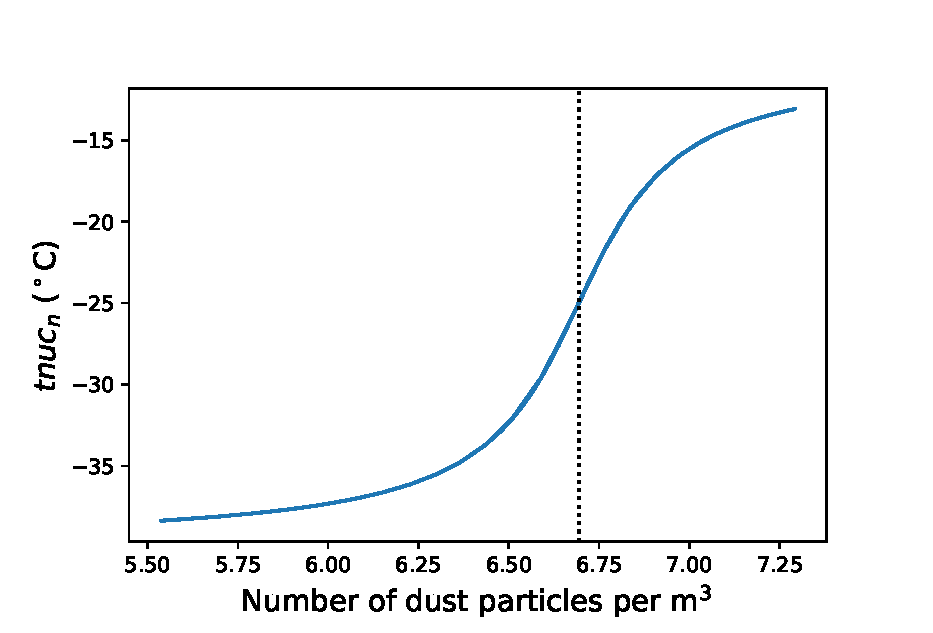
\includegraphics[scale=0.7]{tnuc_new}
        \caption{Representation of $tnuc_n$ vs $dust$ ($log_{10}$ scale)
        following (\ref{eqn:progtnuc}). The dotted line represents the
        arbitrary reference dust value which can be adjusted for testing}
        \label{fig:tnucnew}
    \end{centering}
\end{figure}

In order to implement this approach, the logical switch
{l}\textunderscore{progn}\textunderscore{tnuc} which appears under
Mixed phase processes in Section {04} in rose GUI needs to be set
to true. Additionally, by activating this approach, the
default detrainment temperature thresholds would also be replaced in the
convection scheme. For further details, please refer to \citeumdp{030}.

\subsubsection{PIFRW: Homogeneous nucleation of liquid water}

\textbf{$q_{cl}$ to $q_{cfc}$.} All liquid water at temperatures less than
$-40^{\circ}$C is instantaneously frozen to form ice particles ($q_{cfc}$),
according to \cite{Rogers:Yau:1989}.
In the scheme $C_i$ is set equal to $C$ and $C_l$ set to zero.

\subsubsection{PIFRW: Homogeneous nucleation of liquid water}

\textbf{$q_{cl}$ to $q_{cfc}$.} All liquid water at temperatures less than 
$-40^{\circ}$C is instantaneously frozen to form ice particles ($q_{cfc}$), 
according to \cite{Rogers:Yau:1989}. 
In the scheme $C_i$ is set equal to $C$ and $C_l$ set to zero.

\subsubsection{PIFRR: Homogeneous nucleation of rain}

\textbf{$q_{R}$ to $q_{cfc}$.} As PIFRW, but for rain rather than
liquid water.

\subsubsection{PIPRR: Heterogeneous freezing of rain}

\textbf{$q_{R}$ to $q_{graup}$.} From vn11.2 there is an option to include 
heterogeneous freezing of rain. Following \citealp{Bigg:1953}, the heterogeneous
freezing of rain is given by
\bq
P_{PIPRR}=20\pi\ B^\prime n_{0R}\left(\frac{\rho_w}{\rho}\right)\ 
             \left\{\exp{\left[A^\prime\left(T_0-T\right)\right]}-1\right\}\lambda_R^{-7}
\label{eq:mic_rainfreeze}
\eq
where $A^\prime$ and $B^\prime$ are parameters determined by
laboratory experiments and defined as $0.66$ \textdegree C$^{-1}$ 
and 100 $m^{-3}~ s^{-1}$ respectively,
and $T_0-T$ is the difference between $0$ \textdegree C and the temperature.

The heterogeneous freezing rain term is only active if the temperature is 
$< -4$ \textdegree C and the rain water mixing ratio exceeds a small 
threshold of $1\times10^{-8}~kg~ kg^{-1}$.

If graupel is being used $P_{PIPRR}$ is a source term for graupel, otherwise it is 
a source term for ice aggregates. 

\textbf{Cloud fraction changes} There is no change to the rain fraction from 
this term, except if all of the rain freezes $C_R$ is set to $0$.
If using the prognostic precipitation fraction, the change of rain fraction
is calculated differently; see section \ref{sec:precip_frac_update}.
If this term acts as a source of ice aggregates, the ice cloud fraction after this
process is taken to be the $\mmax {C_R,C_i}$, which assumes that nucleation
occurs throughout the rain volume. 

\subsubsection{PSDEP/PSSUB:  Deposition/Sublimation of vapour on to aggregates}
\label{sec:psdep_pssub}

\textbf{$q_{cl}$ to $q_{cfa}$, $q$ to $q_{cfa}$.} The deposition/sublimation 
equation is
(following \citealp{Rogers:Yau:1989} or \citealp{Rutledge:Hobbs:1983}): 
\bq
      \frac {dM_{x}}{dt}=\frac{ \left(\frac{q}{q_{isat}}-1\right)}
                           {\mbox{AB}} C F'.
\label{eq:mic_dmevap}
\eq
where $dM_x/dt$ represents the rate of change of mass due to the phase change, 
$\mbox{AB}$ is a function of temperature and is different for ice or
liquid particles, $C$ is
the shape parameter, for spherical particles $C=2 \pi D$, and
$F'$ is the ventilation coefficient. The scheme uses the ventilation
factor of \cite{Thorpe:Mason:1966}, which is applicable for hexagonal plates:

\bq
F'=0.65+0.44S_c^{\frac{1}{3}} R_e^\frac{1}{2}
\eq

where $R_e$ is the Reynolds number given by
\bq
 R_e = \frac{V_x(D) D \rho}{\mu}
\eq

where $\mu$ is the dynamic viscosity of air. The Schmidt number, $S_c$ is set to 0.6
as discussed earlier. 

The integrated value of $CF'$ \textit{for spherical particles} over a generalised
gamma distribution of sizes is defined as:
\bq
  {{\cal V}_x}=2\pi n_{0x}
          \left(0.65\frac{\Gamma(2+\alpha_x)}{\lambda_x^{(2+\alpha_x)}}
                       +0.44\left(\frac{c_x}{\mu}\right)^{\frac{1}{2}}
                                                          S_c^{\frac{1}{3}}
 \rho^{\frac{1}{2}} {\left( \frac{\rho_0}{\rho} \right)}^{\frac{\mathcal{G}_x}{2}}
        \frac{\Gamma\left(0.5d_x+\alpha_x+2.5\right)}
 {\left(\lambda_x+0.5h_x\right)^{(0.5d_x+\alpha_x+2.5)}}
          \right)
\label{eq:mic_ventx}
\eq

 $x$ can stand for $R$,$c$,$a$ or $g$.
The deposition and sublimation rates of snow aggregates
($P_{SDEP}$ and $P_{SSUB}$) are given by

\bq
 P_{SDEP} ( or ~ -P_{SSUB})=
     \frac{ \left(\frac{q}{q_{isat}}-1\right)} {\rho \mbox{AB}_{ice}}
\times {{\cal V}_x}
\label{eq:mic_xsub}
\eq

where $\mbox{AB}_{ice}$ is a thermodynamic term
given by \cite{Rogers:Yau:1989} as

\bq
  \mbox{AB}_{ice}=\left(\frac{L_S}{R_vT}-1\right)\frac{L_S}{K_a(T)T}+\frac{R_v
  T}{e_{isat}\psi(T,p)}
\label{eq:mic_ABiceUM}
\eq

where $e_{isat}$ is the saturated vapour pressure over ice. When liquid exists this
is assumed to be removed before the ice (the Bergeron-Findeisen process: 
\citealp{Bergeron:1935}),
hence the split into $P_{SDEP1}$ and $P_{SDEP2}$ terms. The deposition/sublimation 
term only acts when $T<0 \deg C$.

\textbf{Non-spherical particles}. The above derivation is for spherical particles
(these are used by default but aren't consistent with the area-size relationships).
For non-spherical particles we can use the concept of capacitance to provide
a multiplying factor to the rate equation. This gives \citep{Rogers:Yau:1989}:

\begin{eqnarray}
c =  \frac{  {\left(1 - \left( {\frac{1}{r_a}} \right)^2 \right) }^{ \frac{1}{2}} }
          {\mathrm{log} \left( r_a + {\left( {r_a}^2 -1 \right)}^{\frac{1}{2}} \right)},
          ~~r_a > 1 (prolates) \\
c = 1,~~r_a = 1 (spherical) \\
c = \frac{ {\left( 1 - {r_a}^2 \right)}^{\frac{1}{2}}}
         {\mathrm{sin}^{-1} \left( {\left( 1 - {r_a}^2 \right)}^{\frac{1}{2}} \right) },
          ~~r_a < 1 (oblates) 
\end{eqnarray}

where $r_a$ is the axial ratio\footnote{This is defined as $a/b$ in \cite{Rogers:Yau:1989}
and \cite{pruppacher:klett}. In their notation, $a$ is the major semi-axes while $b$ 
is the minor semi-axes.} 


$c$ is the multiplying factor to apply to ${\cal V}_x$. The 
precipitation scheme allows the specification of an axial ratio and make 
additional assumptions about the nature of the particle shape;
subliming particles are assumed to have a more rounded shape with more 
molecular-scale
surface steps on their surface. This means it is more difficult to deposit ice than
sublime it, and accordingly the rate for depositing ice is multiplied by
a factor of 0.9, which is a number used by Wilson to represent this process.

By default, model assumes all ice crystals to be spherical. To change the capacitance or
shape parameter value for non-spherical particles (i.e. corresponding to any oblate sphere shape in general,
where the horizontal axes are longer than the vertical axis and more representative of an
aggregate or flat ice crystal), the logical switch, 
{l}\textunderscore{ice}\textunderscore{shape}\textunderscore{parameter},
which appears under Ice processes in Section {04} in rose GUI needs to be set to true.

\textbf{With the generic ice particle size distribution} When the
generic ice particle size distribution is switched on, equation \ref{eq:mic_xsub} 
remains identical, but equation \ref{eq:mic_ventx} is modified as

\bq
{{\cal V}_x}=2\pi\left(0.65 \mathcal{M}_1 + 0.44 
\left(\frac{c_x}{\upsilon}\right)^{\frac{1}{2}}S_c^{\frac{1}{3}}\rho^{\frac{1}{2}} 
{\left( \frac{\rho_0}{\rho} \right)}^{ \frac{\mathcal{G}_x}{2}}
\mathcal{M}_{1+0.5(d_a+1)}\right),
\label{eq:mic_ventx_psd}
\eq

where $\mathcal{M}_1$ is the first moment of the generic ice particle size distribution
calculation and $\mathcal{M}_{1+0.5(da+1)}$ is the result of inputting 
$1+0.5~(d_a+1)$ into the generic ice particle size distribution calculation.

The multiplying factor, $c$, for non-spherical particles may also be used to scale
the values coming from equation \ref{eq:mic_ventx_psd}. 

\textbf{Cloud fraction changes} 
Deposition is assumed to remove $C_l$ but not to adjust $C_i$ or $C$. If we assume a
uniform distribution of liquid water across the liquid cloud partition between
values 0 and $\frac{2 q_{cl}}{C_l}$, and a uniform removal of liquid water, then we
obtain the expression

\bq
\Delta C_l = C_l {\left( 1 - \frac{\Delta q_{cl}}{q_{cl}} 
\right) }^{\frac{1}{2}} - C_l .
\eq

Sublimation is assumed to reduce $C_i$ but not to alter $C_l$. A similar argument
to that for deposition allows one to estimate this change as

\bq
\Delta C_i = C_i { \left( 1 + \frac{\Delta q_{cf}}{q_{cf}} \right) }^{\frac{1}{2}}
\eq

and hence a similar adjustment to the total cloud fraction (since sublimation
can only occur outside of liquid cloud). 

\subsubsection{PIDEP/PISUB: Deposition/Sublimation of vapour on to ice crystals}

\textbf{$q_{cl}$ to $q_{cfc}$, $q$ to $q_{cfc}$.}
This term is identical to the above
except the parameters used are
those for the ice crystal category.

\subsubsection{Hallett-Mossop process}

\textbf{Formulation in the UM}

There is functionality in the UM to include a simple
\cite{Hallett:Mossop:1974} process that acts to increase the deposition rate by 
a factor
when supercooled liquid water is present, although this is not usually turned 
on in the model. A gui/namelist switch from VN7.9 allows this option to be turned on
if required.

The deposition rate to ice crystals with the Hallett-Mossop representation
on ($PIDEP_{HM}$) is given by
\bq
PIDEP_{HM} = PIDEP \left( 1 + f_{HM}(T) \frac{q_{cl}}{q_{cl0}} \right)
\eq
where $q_{cl0}$ is a reference liquid water content from 
\citealp{Hallett:Mossop:1974}
($1.0 \times 10^{-4}$ kg kg$^{-1}$) and
$f_{HM}$ is a function of temperature

\begin{eqnarray}
f_{HM} = \frac{1}{HM_{norm}} \left( 1 - \exp \left( \frac{ T - T_{HM2} }{T_{HM3}} 
\right) \right),~~T_{HM2}>T>T_{HM1} \\
f_{HM} = \exp \left( \frac{ T - T_{HM1} }{T_{HM3}} \right), ~~T<T_{HM1} \\
f_{HM} = 0, ~~T>T_{HM2}
\end{eqnarray}
where
\bq
HM_{norm} = 1 - \exp \left( \frac{ T_{HM1} - T_{HM2} }{T_{HM3}} \right).
\eq

$T_{HM1}$ and $T_{HM2}$ are the temperature limits for producing splinters, 
the rate varies  with number concentration over an altitude 
equivalent to a temperature
change of $T_{HM3}$. If you wish to use this representation, you are advised to set
$T_{HM1} = -8~^{\circ}$C, $T_{HM2} = -3~^{\circ}$C, $T_{HM5} = 7~^{\circ}$C.

\subsubsection{PSAUT:  Aggregation of ice crystals to snow aggregates }

\textbf{$q_{cfc}$ to $q_{cfa}$}

\textbf{If there is only one ice prognostic}

The schemes have a diagnostic split between ice crystals and
aggregates and therefore do not include an explicit autoconversion term from
ice crystals to aggregates. Instead, the single ice prognostic variable is split
each timestep into crystals and aggregates for the microphysical 
processes as described earlier.

\textbf{If there are two ice prognostics} 

The process of aggregation of ice crystals to snow 
aggregates is coded to emulate the diagnostic split scheme, i.e. the amount
of ice crystal mass is calculated using the diagnostic split 
(equation \ref{eq:cry_agg_split}) and any mass greater than this threshold is 
transferred to the aggregate category.

\subsubsection{PSACI: Collection of ice crystals by snow aggregates}
\label{sec:PSACI}

\textbf{$q_{cfc}$ to $q_{cfa}$}.
In reality, the
transfer process should be small. This modification only works when the use of 
a second ice prognostic (crystals) is used. Collection of ice crystals by snow
does not take place when the generic ice particle size distribution is turned 
on.

The rate of collision between the snow and ice crystal categories is
parametrized as a double integration, to take into account the spectrum of
sizes of particles of each category.
The general result for the rate that mass from category $y$ is collected 
by category $x$ is

\begin{eqnarray}
 P_{YACX}=\frac{1}{\rho}
          \int_0^\infty\int_0^\infty E_{xy}\frac{\pi}{4}(D_x+D_y)^2
         | V_x(D_x) - V_y(D_y)|
                         \nonumber \\
          \hspace{0.5cm}M_x(D_x) n_x(D_x) n_y(D_y) dD_x dD_y
\label{eq:mic_pyacx1}
\end{eqnarray}

Where $E_{xy}$ is a collection efficiency defined following 
\cite{Gray:etal:2004} as
\bq
E_{xy}= 0.02 \exp ( 0.08 (T - 273.15))
\label{eq:mic_exy}
\eq

The integration of equation \ref{eq:mic_pyacx1} is made easier 
(or indeed possible) by making the assumption of \cite{Forbes:Halliwell:2003}
that

\bq
| v_x(D_x) - v_y(D_y) | =\mmax{(\overline{v_x}+\overline{v_y})/8,| \overline{v_x} 
- \overline{v_y} |}
\label{eq:mic_vx_vy}
\eq

for all values of $D_x$ and $D_y$. So the velocity difference between any two
particles from the two different categories is assumed to be the difference
between the mass--mean fall velocities $\overline{v_x}$ and $\overline{v_y}$ 
or a quarter of the average of the two mass--mean fall velocities, whichever is 
greater. The latter takes account of the distribution of fall speeds in the 
case where the mean fall speeds of the two categories are similar.

Substituting in equation (\ref{eq:mic_vx_vy}) allows equation
(\ref{eq:mic_pyacx1}) to be integrated giving equation \ref{eq:mic_pyacx2} 
(where many of the parameters have been defined earlier in 
section \ref{sec:param_par_char}, with default values 
in tables \ref{tab:mic_consts_psd},\ref{tab:mic_consts_density} and 
\ref{tab:mic_consts_fallspeed}.) Specifically now for the collection
of ice by snow we have: 

\begin{eqnarray}
 P_{SACI}&=&\frac{\pi}{4\rho} E_{xy}a_a n_{0c}\mmax{(V_a+V_c)/8,| V_a -V_c |}
          \nonumber \\
         & &\times\int_0^\infty\int_0^\infty (D_a+D_c)^2
          D_a^{b_a}n_a(D_a) n_c(D_c) dD_a dD_c
          \nonumber \\[0.5cm]
           &=&\frac{\pi}{4\rho}E_{xy}a_a n_{0c}\mmax{(V_a+V_c)/8,| V_a -V_c |}
          \nonumber \\
           & & \times  \int_0^\infty D_a^{b_a} n_a(D_a)
              \left(D_a^2\frac{\Gamma(1+\alpha_c)}{\lambda_c^{(1+\alpha_c)}}
                   +2D_a\frac{\Gamma(2+\alpha_c)}{\lambda_c^{(2+\alpha_c)}}
                +\frac{\Gamma(3+\alpha_c)}{\lambda_c^{(3+\alpha_c)}}\right)dD_a
          \nonumber \\[0.5cm]
          &=&\frac{\pi}{4\rho}E_{xy}a_an_{0a}n_{0c}
                                  \mmax{(V_a+V_c)/8,| V_a -V_c |}
          \nonumber \\
           & &\times
           \left(\frac{\Gamma(1+\alpha_c)}{\lambda_c^{(1+\alpha_c)}}
                 \frac{\Gamma(3+\alpha_a+b_a)}{\lambda_a^{(3+\alpha_a+b_a)}}
               +2\frac{\Gamma(2+\alpha_c)}{\lambda_c^{(2+\alpha_c)}}
                 \frac{\Gamma(2+\alpha_a+b_a)}{\lambda_a^{(2+\alpha_a+b_a)}}
 \right. \nonumber \\ & & \left. \hspace{1.5cm}
                +\frac{\Gamma(3+\alpha_c)}{\lambda_c^{(3+\alpha_c)}}
                 \frac{\Gamma(1+\alpha_a+b_a)}{\lambda_a^{(1+\alpha_a+b_a)}}
                                                           \right)
\label{eq:mic_pyacx2}
\end{eqnarray}

\newpage

\subsubsection{PSACW:  Riming by aggregates}
\label{sec:PSACW}

\textbf{$q_{cl}$ to $q_{cfa}$.}

\textbf{When the generic ice particle size distribution is not used}

Although this term is called 'riming', it obeys a similar process 
(and hence is formulated in the same way), as that for the accretion of 
liquid cloud by falling rain. 

\begin{equation}
 P_{SACW}=\frac{\pi n_{0a} c_a  \Gamma (3+d_a+\alpha_a) E_{aw} q_{cl}}
            {4(\lambda_a+h_a)^{3+d_a+\alpha_a}}
        \left(\frac{\rho_0}{\rho}\right)^{\mathcal{G}_a}
\label{eq:mic_psacw}
\end{equation}

Collision/collection efficiency $E_{aw}$ are also assumed to be 1,
which is not such a reasonable assumption for ice particles since they
have slower fall-speeds (see e.g. \citealp{Mitchell:1996}). 
No change in the cloud fractions are assumed. 
This term is only allowed to act when T$ < 0 ^{\circ}$C.

\textbf{When the generic ice particle size distribution is used}

This follows the same form as equation \ref{eq:mic_psacw}, although with the 
intercepts replaced by moment calculations. Equation \ref{eq:field1} is used
to calculate the moment of the ice particle size distribution corresponding
to $2+d_a$, $\mathcal{M}_{2+d_a}$ and then the riming equation can be modified
as follows:

\begin{equation}
 P_{SACW} = \frac{\pi}{4} c_a \mathcal{M}_{2+d_a} E_{aw} q_{cl}
\left(\frac{\rho_0}{\rho}\right)^{\mathcal{G}_a}.
\label{eq:mic_psacw_psd}
\end{equation}

\textbf{When shape-dependent riming is used}

The default riming parametrization assumes that the ice particles
undergoing collisions are spheres. The parametrization can be modified to
include a power-law dependence of the cross-sectional area on diameter.
The same method is applied for crystals if two ice species are used.
This is implemented via a user-defined cross-sectional area ratio
(the ratio of particle cross-sectional area to that of a sphere
with the same diameter). The cross-sectional area-ratio is given by
$R(D) = a_r D^{b_r}$, the parameters $a_r$ and $b_r$ being user-defined inputs.
In the code, the actual particle area is $A = RD^2$ (a neglected factor
of $4/\pi$ being considered as part of the uncertainity in the
collection efficency of ice/liquid collisions).
The default parameters are taken from the analysis of {\it insitu} aircraft data by \cite{Heymsfield:Milo:2003}.

Using the shape-dependent riming parametrization also allows for
a threshold liquid-water content for riming to be specified. Only
liquid water contents above this threshold are available for riming.
This is done to mimic the findings of \cite{Harimaya:1975}
that there is a minimum droplet size for riming to occur.
To implement the minimum  $q_{cl}$ for riming, the implicit solution of the process rate equation is modified, as described in Section
\ref{sec:proc_rate_implicit}.


\subsubsection{PIACW:  Riming by crystals}

\textbf{$q_{cl}$ to $q_{cfc}$.}
This term is formulated in the same way as 
the riming by aggregates term in equation \ref{eq:mic_psacw}  
(and is valid for non-generic ice PSD cases). The only differences
are the values of the parameters used in the PSD, density and fall speed
parametrizations. Collision/collection efficiency are also assumed to be 1 and
no change in cloud fractions occur.


\subsubsection{PGAUT:  Autoconversion of snow to graupel}
\label{sec:PGAUT}

\textbf{$q_{cfa}$ to $q_{graup}$.}
It is assumed that when snow growth is dominated by riming
liquid cloud it increases its density, so some is converted to the graupel
category. A threshold snow mass concentration is defined which must be
exceeded before this process is activated. This is for 
$\rho q_{cfa} >3 \times 10^{-4}$ kg m$^{-3}$ and also the temperature must be
below 
$-4$\,C. This is based on radar observations of a large number of
convective showers over Southern England \citep{Forbes:Halliwell:2003}. 
The conversion rate is:

\bq
P_{GAUT}= \mathcal{F} \times \mmax{0, P_{SACW}-P_{SDEP}}.
\label{eq:mic_pgaut}
\eq

where $P_{SACW}$ is the rate of riming of snow and $P_{SDEP}$ is the rate of snow 
deposition. Thus the riming rate of snow must exceed the rate of growth due to vapour
deposition. The coefficient $\mathcal{F}$ is inserted because the riming 
snow will not immediately increase its density to that of graupel. For the original
\cite{Forbes:Halliwell:2003} graupel scheme, $\mathcal{F}$ is set to a constant value
of 0.5. With the modified scheme \cite{Field:etal:2019}, the value of $\mathcal{F}$
is set to match the \cite{Thompson:etal:2008} scheme as follows:
\bq
  \mathcal{F}=\left\{ \begin{array}{llll}
      0.75  & & \mathcal{R} & > 30 \\
      0.028 (\mathcal{R} -5) + 0.05 & 5 \le & \mathcal{R} & \le 30 \\
      0     & & \mathcal{R} & < 5
    \end{array},\right.
\label{eq:mic_pgaut_f}
\eq
where $\mathcal{R}$ is defined as $\frac{P_{SCAW}}{P_{SDEP}}$.

This has the impact that the initial snow to graupel production within a cloud cannot 
start until the ratio of riming to deposition is 5 or more. With the original graupel
scheme, small amounts of graupel were commonly produced away from the main core of a 
convective cell; with the modifications in \ref{eq:mic_pgaut_f}, the graupel seen 
within a convective cell tends to be produced closer to the main core of the storm,
which looks more realistic when comparing to radar observations. 

\subsubsection{PGACW: Riming by graupel}
\label{sec:PGACW}

\textbf{$q_{cl}$ to $q_{graup}$.}
The collection rates of liquid cloud by graupel obey exactly the same physics as 
the riming of crystals and aggregates (equation \ref{eq:mic_psacw}, but with
the parameters for graupel from tables \ref{tab:mic_consts_psd} and
\ref{tab:mic_consts_fallspeed} used in place of those for aggregates).  

\subsubsection{PGACS: Collection of snow aggregates by graupel}
\label{sec:PGACS}

\textbf{$q_{cfa}$ to $q_{graup}$.}
The rates of collision between the graupel and snow categories is parametrized
in the same way as the snow/crystal collisions (PSACI) described by equation
\ref{eq:mic_pyacx2} in section \ref{sec:PSACI}, but with the coefficients for 
graupel replacing those for snow aggregates and those for snow aggregates replacing 
those for ice crystals. The collection efficiencies remain the same as those 
used in equation \ref{eq:mic_exy}.

\textbf{With the generic ice particle size distribution}

This uses the same physics, but is calculated slightly differently from 
\ref{eq:mic_pyacx2} in section \ref{sec:PSACI}. Equation \ref{eq:field1}
is used to calculate the zeroth ($\mathcal{M}_0$), first ($\mathcal{M}_1$), 
second ($\mathcal{M}_2$) and $b_a+d_a$ ($\mathcal{M}_{b_a+d_a}$) moments
of the ice distribution. The moment $\mathcal{M}_{b_a+d_a}$ is used to 
calculate the ice particle fall speed, following equation 
\ref{eq:icefallpsd}. 

Equation \ref{eq:mic_pyacx2} is then modified as follows:

\begin{eqnarray}
P_{GACS}  &=&\frac{\pi}{4\rho}E_{xy}a_gn_{0g}
                                  \mmax{(\overline{v_g}+\overline{v_a})/8,| 
\overline{v_g} -\overline{v_a} |}
          \nonumber \\
           & &\times
           \left(\mathcal{M}_0
                 \frac{\Gamma(3+\alpha_g+b_g)}{\lambda_g^{(3+\alpha_g+b_g)}}
               +2\mathcal{M}_1
                 \frac{\Gamma(2+\alpha_g+b_g)}{\lambda_g^{(2+\alpha_g+b_g)}}
 \right. \nonumber \\ & & \left. \hspace{1.5cm}
                +\mathcal{M}_2
                 \frac{\Gamma(1+\alpha_g+b_g)}{\lambda_g^{(1+\alpha_g+b_g)}}
                                                           \right)
\label{eq:pgacs_psd}
\end{eqnarray}

\textbf{With the increased graupel production option and the improved graupel 
representation}

Two options exist to alter the graupel parametrization from the 
\cite{Forbes:Halliwell:2003} representation. The first is an increased
production of graupel option where snow-rain collisions are allowed to
create graupel in place of snow. The second is an improved graupel
particle size distribution shown as option (ii) within table
\ref{tab:mic_consts_psd} and based on the work by \cite{Field:etal:2019}. 

When either of these two options are in use, the $P_{GACS}$ term above 
defaults to 0.0. This is based on personal communication with Gregory Thompson 
(NCAR) who believes that collisions between graupel and snow particles do not 
result in any changes in the form of ice. Therefore, when either of these
two options is se, there will be no change in graupel or snow masses due
to the collection of snow aggregates by graupel.

\subsubsection{PSACR:  Collection of rain by aggregates}
\label{sec:PSACR}

\textbf{$q_{R}$ to $q_{cfa}$.}
This term uses similar assumptions as for the collection of ice crystals by 
snow aggregates above (equation \ref{eq:mic_pyacx2} in section \ref{sec:PSACI}). 
Again, the approximation
\bq
f_V = \mmax{| \overline{v_a} - \overline{v_R} |,  \frac{ \overline{v_a} + 
\overline{v_R} }{8}~}
\eq
is used and the collision and collection coefficients are now assumed to be 1.
Integrating leads to terms in $\lambda_R$ and $\lambda_a$ which can then be 
solved:

\begin{eqnarray}
P_{SACR}& =& 
\frac { \pi^{2} \rho_w f_V } {24 \rho } n_{aa} \lambda_a^{n_{ba}} n_{aR} 
\lambda_R^{n_{bR}} \nonumber \\
& & \times
\left(\frac{\Gamma(3+\alpha_a) \Gamma(4+\alpha_R)} 
{\lambda_a^{3+\alpha_a} \lambda_R^{4+\alpha_R}}
+ \frac{ 2 \Gamma(2+\alpha_a) \Gamma(5+\alpha_R) } 
{\lambda_a^{2+\alpha_a} \lambda_R^{5+\alpha_R}} \right. \nonumber \\
& & \left. \hspace{1.5cm}+ \frac{\Gamma(1+\alpha_a) 
\Gamma(6+\alpha_R)} { \lambda_a^{1+\alpha_a} \lambda_R^{6+\alpha_R} }
\right)
\label{eq:psacr}
\end{eqnarray}

Note that equation \ref{eq:psacr} is formulated slightly differently than equation 
\ref{eq:mic_pyacx2} due to the captured quantity being water and not ice.


\textbf{When the increased graupel production term is included}
The resultant of the collision/collection $P_{SACR}$ can either be aggregates 
or graupel. Collisions that produce graupel are noted $P_{SACR-G}$ whilst those
which produce aggregates are noted $P_{SACR-A}$. If the increased graupel 
production scheme (allowing snow-rain collisions to
produce graupel) is switched off, then the collision will not produce any graupel 
(i.e. the result is always $P_{SACR-A}$). 

If the scheme is switched on, then collisions between aggregates and rain will 
always produce graupel.
 
\textbf{Aside:} Note that a different sub-routine is used dependent on
whether the collection/captured quantity is between rain and ice. 
\textit{lsp\_collection.F90} is used for ice-ice processes, 
\textit{lsp\_capture.F90} is for ice-liquid processes and liquid-liquid 
(accretion) is in \textit{lsp\_accretion.F90}.

There is no update to the rain fraction $C_R$ from this process.
However, in the event that collection of rain reduces qrain to zero,
checks later in the microphysics scheme will reset the rain fraction to zero.

If using the prognostic precipitation fraction, the change of rain fraction
is calculated differently; see section \ref{sec:precip_frac_update}.

There are no changes to the cloud fractions
as a result of this process.

\textbf{When the generic ice particle size distribution is used}

This is calculated in a similar way to section \ref{sec:PGACS}. 
Equation \ref{eq:field1} is used to calculate the zeroth ($\mathcal{M}_0$), 
first ($\mathcal{M}_1$), second ($\mathcal{M}_2$), $1+0.5(d_a+1)$ 
($\mathcal{M}_{1+0.5(d_a+1)}$) and $b_a+d_a$ 
($\mathcal{M}_{b_a+d_a}$) moments of the ice distribution. The moment 
$\mathcal{M}_{b_a+d_a}$ is used to calculate the ice aggregate fall speed, 
following equation \ref{eq:icefallpsd}. 

Equation \ref{eq:psacr} can be modified as follows

\begin{eqnarray}
P_{SACR}& =& \frac { \pi^{2} \rho_w f_V } {24 \rho }  n_{aR} \lambda_R^{n_{bR}} 
\nonumber \\
& & \times
\left(\frac{\mathcal{M}_2 \Gamma(4+\alpha_R)} {\lambda_R^{4+\alpha_R}}
+ \frac{ 2 \mathcal{M}_1 \Gamma(5+\alpha_R) } {\lambda_R^{5+\alpha_R}} \right. 
\nonumber \\
& & \left. \hspace{1.5cm}+ \frac{\mathcal{M}_0 \Gamma(6+\alpha_R)}
{\lambda_R^{6+\alpha_R} } \right)
\label{eq:psacr_psd}
\end{eqnarray}

where, as usual the moments replace the aggregate terms.

When the generic ice particle size distribution is used in conjunction 
with the increased graupel production scheme (allowing snow-rain collisions to produce 
graupel) then a different approach must be used due to the lack of an ice
crystal category. This is done by comparing the mean diameters of each of 
the species involved in the collision.

For rain, we can derive the mass-mean diameter as
\begin{eqnarray}
\label{rain:mmd}
\bar{D_R}& = & \frac{\int_0^{\infty} n_{aR} \lambda_R^{n_{bR}} \frac{\pi}{6} \rho_w D_R^3 
\exp(-\lambda_R D) D dD }
{\int_0^{\infty} n_{aR} \lambda_R^{n_{bR}} \frac{\pi}{6} \rho_w D_R^3 
\exp(-\lambda_R D) dD } \nonumber \\
         & = & \frac{\int_0^{\infty} D^4 \exp(-\lambda D) dD }
                    {\int_0^{\infty} D^3 \exp(-\lambda D) dD } \nonumber \\
         & = & \frac{\Gamma(5)}{\lambda_R^5} \frac{\lambda_R^4}{\Gamma(4)} \nonumber \\
         & = & \frac{4}{\lambda_R} 
\end{eqnarray}

The value of $\lambda_R$ can then be derived as in section \ref{mr2psd}. A similar
approach can be used to define 4.0/$\lambda_R$ for aggregates. This is simply 
as follows
\begin{eqnarray}
\label{ice:mmd}
\bar{D_a}& = & \frac{4}{\lambda_a}\nonumber \\
         & = & \frac{\mathcal{M}_{ba + 1}}{\mathcal{M}_{ba}}
\end{eqnarray}
where equation \ref{eq:field1} is used to calculate the two moments required.
If $\bar{D_R}$ is greater than $\bar{D_a}$ then the result of a collision is
a graupel particle. Otherwise the result will be an ice aggregate.

\subsubsection{PIACR:  Collection of rain by crystals}

\textbf{$q_{R}$ to $q_{cfc}$.}
This term is formulated in the same way as the
collection of rain by aggregates term (PSACR; equation \ref{eq:psacr} in 
section \ref{sec:PSACR}). The only differences are the values of
the parameters used to describe the properties of the crystals.

\textbf{With the increased graupel production option}
Collisions between crystals and rain will produce
graupel ($P_{IACR-G}$) if the rain mixing ratio is 0.1 g kg$^{-1}$ or above. 
Below this threshold the result of the collision will be crystals 
($P_{IACR-C}$).

\subsubsection{PSMLTEV: Evaporation of melting snow aggregates}

\textbf{$q_{cfa}$ to $q$.}
This term acts to evaporate any ice at temperatures above 0\textdegree C since
the deposition term is switched off at these temperatures. The term follows that
for the deposition/sublimation process equation with the exception that
saturation vapour pressures and latent heats in the calculation of the
evaporation rate are used for liquid, not ice. However, the latent heat of
sublimation is used to calculate the temperature change due to the evaporation.
Either the default `intercepts' method or the generic ice particle size 
distribution can be used with this option; the formulation is the same as
in section \ref{sec:psdep_pssub}.


\subsubsection{PIMLTEV:  Evaporation of melting ice crystals}

\textbf{$q_{cfc}$ to $q$.}
This term is parametrized in the same way as for aggregates, simply with the 
crystal parameters instead of the aggregate values.

\subsubsection{PSMLT:  Melting of snow aggregates to rain}

\textbf{$q_{cfa}$ to $q_R$.}
This is solved from the diffusion equation. The latent heat due to melting is
equal to the sum of the sensible heat lost due to thermal diffusion and
convection and the latent heat due to vapour transfer:
\bq
 L_f \frac {dM_{melt}}{dt}=-2\pi D K_a T_c F'
                   +2\pi D L_v \psi \rho (q - q_{0sat}) F'
\eq
Here, $q_{0sat}$ is the saturation mixing ratio at 0 $^{\circ}$C.
Integrating over all particle diameters, and ignoring corrections due
to the sensible heat associated with accreted liquid water, the melting of
snow to form rain is given as:
\bq
 P_{SMLT} ~=~
\frac{1}{\rho L_f} (K_a(T-T_0)-L_v\psi\rho(q -q_{0sat}))\times{\cal V}_a
\label{eq:mic_psmlt}
\eq

where $T_0$ is 0\textdegree C. The ventilation coefficient is given in equation
\ref{eq:mic_ventx}. The second term can be subsumed into the first
if we use the wet-bulb temperature, $T_w$, in the calculation. Damian Wilson 
approximated the wet bulb temperature over a range of temperatures and pressures 
as
\begin{equation}
T_w-T_0 = T - T_0 + \left( q_{wsat} - q \right) \times
\left(\mathcal{N}_1 + \mathcal{N}_2 (p - \mathcal{N}_3)
 - \mathcal{N}_5 (T - \mathcal{N}_6) \right) .
\end{equation}

where $\mathcal{N}_1= 1329.31$ K, $\mathcal{N}_2=0.0074615$ K m$^2$ N$^{-1}$,
$\mathcal{N}_3= 0.85 \times 10^5 $ N m$^{-2}$, $\mathcal{N}_5= 40.637 $ and
$\mathcal{N}_6=275$K. The variable $q_{wsat}$ is the saturation mixing ratio
with respect to liquid water.

The value of $T_w$ used in the calculation is
weighted by the size of the ice-only and the mixed-phase partitions in the gridbox.
The rain fraction is increased to $C_i$ if $C_i$ is larger
than the rain fraction.
If using the prognostic precipitation fraction, the change of rain fraction
is calculated differently; see section \ref{sec:precip_frac_update}.
The scheme reduces the $C_i$ in proportion to the
mass of ice melted:
\bq
\Delta C_i = P_{SMLT} \frac{C_i}{q_{cfa}}
\eq
and reduces $C$ assuming that the changes to $C_i$ are randomly overlapped with
any existing liquid cloud.

\textbf{Using the generic ice particle size distribution}

This follows the intercept method, although with the ventilation coefficient
as defined in equation \ref{eq:mic_ventx_psd}.


\subsubsection{PIMLT:  Melting of ice crystals to rain}

\textbf{$q_{cfc}$ to $q_{R}$.} 
This term is equivalent to the melting of aggregates to rain,
although with different parameter values.

\subsubsection{PGMLT:  Melting of Graupel}
\label{sec:PGMLT}

\textbf{$q_{graup}$ to $q_{R}$.}
The melting of graupel acts as a source of rain and is parametrized in the same 
way as the melting of snow to form rain in the UM:
\bq
 P_{GMLT} =
\frac{1}{\rho L_f} K_a(T_w-T_0) \times{\cal V}_g ,
\eq
where $L_f$ is the latent heat of fusion, $K_a$ is the thermal conductivity,  
$(T_w-T_0)$ is the difference between the wet-bulb temperature of the air 
and 0\textdegree C and ${\cal V}_g$ is the integrated ventilation factor for 
spherical particles with a generalised gamma distribution of particle sizes:
\bq
  {{\cal V}_g}=2\pi n_{0g}
          \left(0.78\frac{\Gamma(2+\alpha_g)}{\lambda_g^{(2+\alpha_g)}}
                       +0.31\left(\frac{c_g}{\mu}\right)^{\frac{1}{2}}
                                                          S_c^{\frac{1}{3}}
         \rho^{\frac{1}{2}}\left(\frac{\rho}{\rho_0}\right)^{\frac{\mathcal{G}_g}{2}}
        \frac{\Gamma\left(0.5d_g+\alpha_g+2.5\right)}
 {\left(\lambda_g+0.5h_g\right)^{(0.5d_g+\alpha_g+2.5)}}
          \right).
\label{eq:mic_ventx_g}
\eq 
It should be noted that the ventilation coefficients used here, (0.78 and 0.31)
are the same as rain and not ice. This method is used elsewhere in the literature 
(e.g. \citealp{Reisner:etal:1998} ) and tries to implement the fact that graupel
particles are spheres with a much higher density than aggregates, and are more
like raindrops in nature than they are like aggregates. 

\subsubsection{PREVP:  Evaporation of rain}
\label{sec:PREVP}

\textbf{$q_{R}$ to $q$.}
The evaporation rate of rain is analogous to the sublimation of snow in
equation (\ref{eq:mic_xsub}) and only occurs in sub-saturated air.
\bq
 P_{REVP}=
     \frac{ \left(\frac{q}{q_{wsat}}-1\right)} {\rho \mbox{AB}_{liq}}
\times {{\cal V}_r}
\eq
where $\mbox{AB}_{liq}$ is the thermodynamic coefficient appropriate for
liquid drops and is given by,
\bq
\mbox{AB}_{liq}=   \left(  \frac{L_v}{R_v T} -1 \right) 
\frac{L_v}{K_a T} + \frac{R_v T}{\psi e_{sat~liq}}.
\label{eq:mic_ABliq}
\eq

There are a few differences to the sublimation term.
The ventilation factor is different, in this term
we use the \cite{Beard:Pruppacher:1971} formulation:
\bq
F'=0.78+0.31S_c^{\frac{1}{3}} R_e^\frac{1}{2}
\eq
where the Schmidt number, $S_c$, is again approximated to the value 0.6. 
The particles are also assumed to be spherical in the capacitance
calculation.

Note that if the user has diagnostic rain selected and 
the \cite{Abel:Shipway:2007} rain fall speeds selected, the evaporation rate 
will be enhanced for light rain rates, in an attempt to remove some of the 
spurious drizzle from the model. See section \ref{sec:as07} for more details.

Usually this process does not alter the rain fraction $C_R$;
except that $C_R$ is reset to zero in the event that qrain falls below
a minimum allowed value, below-which it is forced to evaporate completely.

If using the prognostic precipitation fraction, the change of rain fraction
is calculated differently; see section \ref{sec:precip_frac_update}.

There are no cloud fraction changes associated with this term.

\subsubsection{PRACW:  Accretion of cloud liquid water by rain}
\label{sec:PRACW}

\textbf{$q_{cl}$ to $q_{R}$.}
The rate that liquid cloud is collected by rain is the product of the sweep out
rate of rain, the mass concentration of liquid cloud and the efficiency that
liquid cloud droplets collide with and then coalesce with raindrops that intercept
them on their direct fall line. This is formulated as:
\begin{equation}
 P_{RACW}=\frac{\pi n_{0r} c_r  \Gamma (3+d_r+\alpha_R) E_{rw} {q_{cl}}}
            {4(\lambda_R+h_R)^{3+d_r+\alpha_R}}
        \left(\frac{\rho_0}{\rho}\right)^{\mathcal{G}_R}
 \label{eq:mic_pracw}
\end{equation}

We assume that the collision/collection efficiency is 1. There is assumed to
be no change in rain fraction and no change in cloud
fractions.

{\bf Under the improved warm rain scheme}, this process rate is
replaced by the formulation of \cite{Khair:Kogan:2000}, bias corrected
following \cite{boutle:etal:2014}. Therefore, the process rate is
given by:
\begin{equation}
  P_{RACW} = 67E(f_{cl},f_R,\rho)q_{cl}^{1.15}q_R^{1.15},
\end{equation}
where
\begin{eqnarray}
E(f_{cl},f_R,\rho)=\qquad\qquad\qquad\qquad\nonumber\\
(1+f_{cl}^2)^{-1.15/2}(1+f_{cl}^2)^{1.15^2/2}\nonumber\\
\times (1+f_R^2)^{-1.15/2}(1+f_R^2)^{1.15^2/2}\nonumber\\
\times \exp\left(\rho 1.15^2 \sqrt{\ln(1+f_{cl}^2)\ln(1+f_R^2)}\right),
\end{eqnarray}
\begin{equation}\label{eq-fsdqcl}
  f_{cl}=\left\{ \begin{array}{ll}
      (0.45-0.25C_l)\sqrt{(xC_l)^{2/3}}((0.06xC_l)^{1.5}+1)^{-0.17}&C_l<1 \\
      0.11\sqrt{(xC_l)^{2/3}}((0.06xC_l)^{1.5}+1)^{-0.17}&C_l=1
    \end{array},\right.
\end{equation}
and
\begin{equation}\label{eq-fsdqr}
  f_R=\left\{ \begin{array}{ll}
      (1.1-0.8C_R)\sqrt{(xC_R)^{2/3}}((0.11xC_R)^{1.14}+1)^{-0.22}&C_R<1 \\
      0.3\sqrt{(xC_R)^{2/3}}((0.11xC_R)^{1.14}+1)^{-0.22}&C_R=1
    \end{array},\right.
\end{equation}
and $\rho=0.9$ is specified.

\subsubsection{PRAUT:  Autoconversion of cloud liquid water to rain}
\label{sec:PRAUT}

\textbf{$q_{cl}$ to $q_{R}$.}
The UM has a power-law formulation of autoconversion as a function of liquid
water content with a minimum threshold liquid water content.

The conversion rate is based on that specified by \cite{Tripoli:Cotton:1980}:
\begin{equation}
P_{RAUT}=A_1 E_{auto} (\rho q_{cl})^{A_2-1} \frac{q_{cl}}{ (n_d)^{A_3}}	
\end{equation}
where $n_d$ is the number of water droplets and $E_{auto}=0.55$ represents a
collision/collection coefficient.
The parameter $A_1$ is defined as

\bq
A_1 = \frac{4 \pi g}{18 {\left(\frac{4}{3} \pi \right)}^{\frac{4}{3}} 
\mu {\rho_{w}}^{\frac{1}{3}}}
\eq

which has the numerical value 5907.24 at $0^{\circ}$C. The other parameters have the
values $A_2 = \frac{7}{3}$ and $A_3=\frac{1}{3}$

There is
a minimum liquid water mixing ratio threshold, $q_{cl0}$ (units of kg kg$^{-1}$), 
for autoconversion to occur. 

\textbf{Default Scheme:}
$q_{cl0}$ is
defined as the liquid water content such that the number concentration of
particles of radii 20 $\mu$m or larger is 1000 m$^{-3}$. The number of droplets
of radius greater than $r$ ($n_r$) can be estimated assuming a modified gamma 
cloud droplet distribution \citep{pruppacher:klett} and then integrating from r to
infinity:
\bq
n_r = \left(\frac{A}{B}\right) r^2 e^{-Br} + \frac{2A}{B^2} r e^{-Br} 
+ \frac{2A}{B^3} e ^{-Br}
\eq
where $A = \frac{B^3 n_d}{2}$, $B=\frac{3}{r_{mean}}$ and 
$r_{mean}= {\left( \frac{27 \rho q_{cl}}{80 \pi \rho_{w} n_d} \right)}^{\frac{1}{3}}$

This can be inverted for a threshold radius of 20 $\mu$m and a threshold 
concentration of 1000 m$^{-3}$ using the following numerical approximation 
(from Andy Jones): 
\begin{eqnarray}
\label{eq:jones_nd}
q_{cl0} &=& \frac{1}{\rho} \left(6.20\times10^{-31} n_d^3 - 5.53\times10^{-22} n_d^2 
\right. 
\nonumber \\
& & \left. + ~4.54\times10^{-13} n_d + 3.71\times10^{-6} - \frac{7.59}{n_d} \right)
\end{eqnarray}
where $n_d$ is in units of m$^{-3}$. The value of $n_d$ is determined in section
\ref{sec:cloud_drop_calc}.

\textbf{\cite{Tripoli:Cotton:1980} autoconversion threshold:}
$q_{cl0}$ is
defined as
\bq
\label{eq:tc_act}
q_{cl0} = \frac{4}{3} \pi \frac{\rho_{w} r^3_{crit} n_d}{\rho}
\eq
where $r_{crit} = 7 \times 10^{-6}$ m and $n_d$ is defined in section 
\ref{sec:cloud_drop_calc}; this was the only option available in the now-retired 
3B scheme.

With both the default, and Tripoli and Cotton autoconversion thresholds, 
autoconversion will not reduce the liquid water content to below the value 
of $q_{cl0}$.

{\bf Under the improved warm rain scheme}, this process rate is
replaced by the formulation of \cite{Khair:Kogan:2000}, bias corrected
following \cite{boutle:etal:2014}. Therefore, the process rate is
given by:
\begin{equation}
P_{RAUT}=1350E(f_{cl})q_c^{2.47}N_c^{-1.79},
\end{equation}
where
\begin{equation}
E(f_{cl})=(1+f_{cl}^2)^{-2.47/2}(1+f_{cl}^2)^{2.47^2/2},
\end{equation}
and $f_{cl}$ is given in Equation~\ref{eq-fsdqcl}.

%
\begin{figure}[t!]
\begin{center}
\subfigure{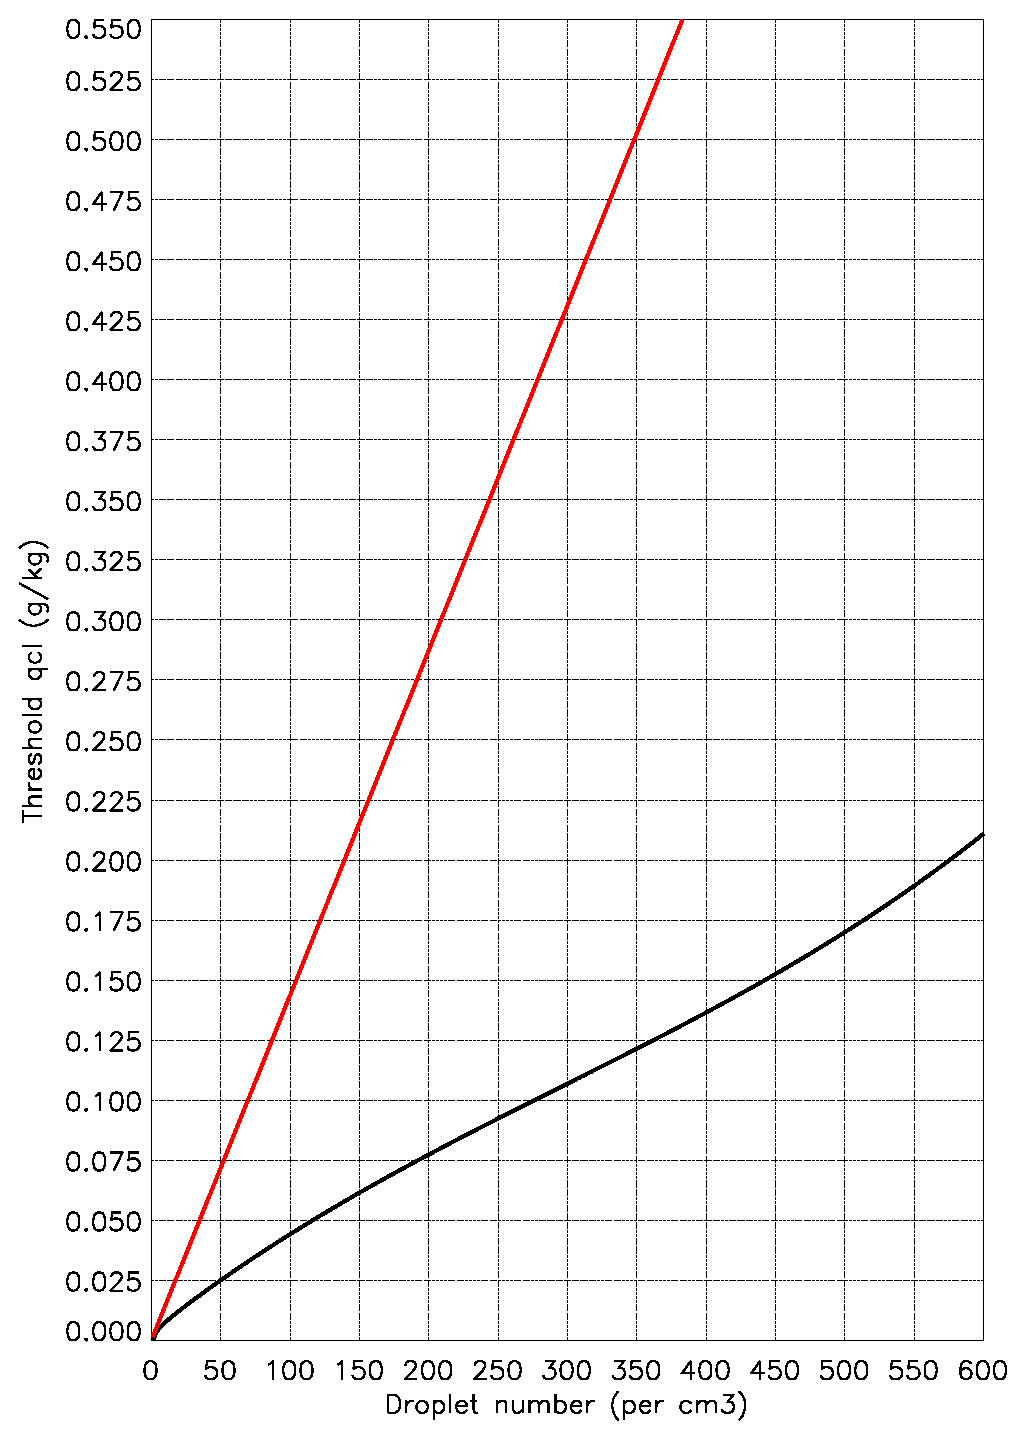
\includegraphics[width=120mm]{autoc_thr}}
\caption{\label{fig:fall_speeds}\footnotesize
  {Autoconversion Thresholds for the default scheme (black line; equation 
\ref{eq:jones_nd}) and the \cite{Tripoli:Cotton:1980} formula (red line; equation 
\ref{eq:tc_act}), shown as a function of cloud droplet number. }}
\end{center}
\end{figure}
%

\textbf{Cloud and rain fractions}. The rain fraction is
increased to $C_l$ if $C_l$ is greater than the current rain fraction.
If using the prognostic precipitation fraction, the change of rain fraction
is calculated differently; see section \ref{sec:precip_frac_update}.

The cloud fractions are not altered by this microphysical process.

\subsubsection{Scavenging of aerosol}
\label{sec:scav}

In addition to the link between MURK aerosol and cloud droplet number 
concentration described in section \ref{sec:PRAUT}, falling precipitation 
particles can remove aerosol (sometimes called scavenging). Rain-out of most 
aerosol species is covered in the appropriate documentation (\citeumdp{020}). 
However, in the case of MURK aerosol, this follows the method of 
\cite{Clark:etal:2008}, and the mixing ratio of aerosol, $A_{mass}$ is
reduced as:  

\begin{equation}
\label{eq:scav}
\frac{A_{mass}}{1.0+K_{rain}RR+K_{snow}SR+K_{ds}PLSET}
\end{equation}

Where $RR$ is the rain rate, $SR$ is the snow rate and $PLSET$ is the 
droplet settle rate. The other coefficients can be described as
\begin{equation}
\label{eq:scav_coef}
K_{rain}=K_{snow}=K_{ds}=1.0\times10^{-4}\times 3600 \times \Delta t.
\end{equation}

\newpage

\section{Numerical methods}

This section briefly describes some of the numerical methods that are used in
the solution of the transfer equations.

\subsection{Fall of ice}

The fall of ice is a particular problem to a microphysics scheme. The model
levels are close together near the surface (less than 100 m apart) and the
timestep may be (in the climate model) as much as 30 minutes. This means that
ice should be able to fall through several model levels in one timestep.

To solve this we look at the rate of change of ice mass (in either the `crystals'
or the `aggregates' category) contained in a layer:

\bq
\rho \Delta z \frac{\partial q_{cfx}}{\partial t} ~=~ S_x - 
\overline{v_{1x}} ~\rho~ q_{cfx}
\eq

where $\overline{v_{1x}}$ is the mean ice fall speed out of the layer and $S_x$
is the snowfall rate into the layer. If we assume that $S_x$ and  
$\overline{v_{1x}}$
are continuous with time (which is true in a steady state) we can solve this
equation as:

\bq
q_{cfx}(t+\Delta t) = \frac{S_x}{\rho \overline{v_{1x}}} (1 - a) + q_{cfx}(t) a
\eq

where $a$ is given by

\bq
a = \exp \left( - \frac{\overline{v_{1x}} \Delta t}{\Delta z} \right) .
\eq

By conservation of ice mass we can deduce that the snowfall rate out of the
layer \\
(~$S_x(z-\Delta z)$~) can be written as:

\bq
S_x(z-\Delta z) = S_x(z) - \left( q_{cfx}(t+\Delta t) - q_{cfx}(t) \right) 
\frac{ \rho \Delta z}{\Delta t}
\eq

which gives a solution

\bq 
S_x(z-\Delta z) = S_x(z) + \frac{\Delta z}{\Delta t} \left( q_{cfx} \rho
- \frac{S_x(z)}{\overline{v_{1x}}} \right) \left( 1 - a \right) .
\eq

This solution will have numerical difficulties if we define $\overline{v_{1x}}$ 
as the mean fall-speed of the ice that starts in a particular layer and $q_{cfx}$ 
in this layer is zero. Accordingly we define $\overline{v_{1x}}$ as an average 
of the fall speed in the layer and that of $\overline{v_{1x}}$ from the layer 
above:

\bq
\overline{v_{1x}}(z) = \frac{ \overline{v_{x}} q_{cfx} + 
\overline{v_{1x}}(z+\Delta z) S_x \frac{\Delta z}{\rho \Delta t} } {q_{cfx} + 
S_x \frac{\Delta z}{\rho \Delta t}  } .
\eq

Since we only store one snowfall flux and one value of $\overline{v_{1}}$ from
layer to layer, we average $\overline{v_{1a}}(z)$ and $\overline{v_{1c}}(z)$
according to the relative mass fractions of aggregates and crystals. Similarly,
$S_a$ and $S_c$ are apportioned from $S$ using the same mass fraction.

The formulation introduces a significant amount of numerical dispersion when
a single `block' of ice is advected downwards.
Although this is not desirable from a numerical point of view (a semi-Lagrangian
scheme may be better, although more expensive to implement), Forbes has
shown that the amount
of dispersion is fortuitously similar to the amount of physical dispersion that should
occur because of the distribution of ice particle sizes (and hence fall
speeds).

\subsection{Implicit formulation}
\label{sec:proc_rate_implicit}

Certain transfer terms, notably those whose rates are proportional to the
amount of a particular variable, can be solved with an implicit timestep,
rather than an explicit one. One example is the riming term. This can be
simplified to the general form:
\bq
\frac{\partial q_{cl}}{\partial t} ~=~ - k~q_{cl}
\eq
where $k$ can be considered a constant (it actually depends on the ice content etc.).
The exact solution would take the form of an exponential decay.
The explicit solution is:
\bq
q_{cl} (t+\Delta t) ~=~ q_{cl} (t)( 1~-~ k \Delta t)
\eq
which would be a reasonable solution if $q_{cl}$ is being continuously replenished
by another process (this cannot be guaranteed, though). The implicit solution
which is used in the code is to approximate the solution as:
\bq
q_{cl} (t+\Delta t) ~=~ q_{cl} (t) \frac{1}{1 ~+~ k \Delta t}
\eq
which will not allow $q_{cl}$ to go negative. A first order binomial expansion
of the implicit solution will retrieve the explicit solution.

Other terms
which are formulated implicitly include the melting term. Here, the rate
is proportional to the temperature difference between the wet-bulb temperature and
the melting point of ice, and this forms the implicit part of the
calculation. Not all the transfer terms are coded in an implicit formulation, so
the advantages of this formulation are likely to be limited.

\textbf{Implicit solution for riming with $q_{cl}$-threshold}

When the shape-dependent riming with liquid water content threshold
(Section \ref{sec:PSACW}) is used, the implicit solution needs
to be modifed to account for the minimum $q_{cl}$ available for riming.
If the $q_{cl}$ threshold is $q_{cl,min}$ then the implicit solution is
\bq
 q_{cl} (t+\Delta t) ~= \min \left\{ q_{cl}(t), \frac{q_{cl}(t)+k\Delta t q_{cl,min}}{1+k\Delta t} \right\}.
\eq

\subsection{Sequential solution of process transfers}
The transfer processes are calculated sequentially in the model. The sequential
updating allows easier coding of limit relationships when two or more processes
compete for water in the same category. For larger timesteps the sequence is
important (although placing transfers in parallel does not guarantee less timestep
sensitivity). Where applicable, in the sequences described below, the transfer for 
the `crystals' is performed before the transfer for the `aggregates'.

\subsubsection{Historic order of transfer processes}
\label{sec:historic_order}
The historic order in which the transfer processes are applied is as follows:\\
Droplet settling, Fall of ice, rain and graupel, Homogeneous nucleation, 
Heterogeneous nucleation, Deposition / Sublimation, Aggregation, 
Crystal collection by aggregates, Riming, Graupel autoconversion, Graupel Riming, 
Graupel collection, Capture, Evaporation of melting snow, Melting, Evaporation of rain, 
Accretion, Autoconversion.

The location of the sedimentation at the start of the microphysics was chosen because early
investigations suggested that having the sublimation term later in the microphysics allows
ice to evaporate on a reasonable depth scale.

\subsubsection{Sedimentation at end of the microphysics}
\label{sec:sed_at_end}

Later, investigations using prognostic rain have shown that the fall of rain being at
the start of the timestep has caused problems. This is because the melting term occurs
after the sedimentation, leading to a collection of stagnant rain at the melting level,
which cannot fall any further until the next call to the microphysics. This stagnant rain
leads to a large radar reflectivity signal at the melting level which looks unrealistic
compared to observations\footnote{This should not be confused with the radar bright-band,
which would not normally be present in model data is and regularly filtered out of radar
observations}. In addition, the stagnant rain at the end of the timestep is passed to
the UM's dynamical core and in the presence of an updraught, will be advected back
above the freezing level, leading to supercooled rain, which may persist to very low
temperatures.

To try and avoid these issues, new options are now available to re-order the transfer
processes using the option \textit{sediment\_loc}. These are as follows:
\begin{enumerate}
\item As the historical order in section \ref{sec:historic_order}.
\item As 1., but with the fall of ice, rain and graupel moved after autoconversion.
\item As 1., but with the droplet settling and fall of ice, rain and graupel
moved after autoconversion.
\item As 1., but with the fall of rain moved after autoconversion.
Fall of ice and graupel remain as the historic order in section \ref{sec:historic_order}.
\item As 4., but with the droplet settling moved between the autoconversion term and the
fall of rain term.
\end{enumerate}


It is recognised that moving the droplet settling and sedimentation terms after the
autoconversion and accretion terms may have a significant impact on fog forecasts
in the UM. Therefore, the order of terms within the microphysics scheme remains a
current area of research.

\subsubsection{Applying process rates to hydrometeor fall-fluxes.}
\label{sec:proc_fluxes}

The ordering of processes detailed in section \ref{sec:historic_order} can
be summarised as:
\begin{enumerate}
\item Add fall-in of precip flux from the level above.
\item Subtract fall-out of precip flux to the level below.
\item Various process rates applied to the mass of hydrometeors remaining
on the current model-level
(autoconversion, accretion, riming, evaporation, vapour-deposition, etc).
\item Tidy-up.
\end{enumerate}

This ordering of processes means that rain, graupel, snow etc can fall
{\em through} a model-level {\em before} any of the process rates are applied
(the fall-out flux calculated at stage (2) above cannot be modified by any of
the subsequent processes, such as rain evaporation).
This leads to various numerical problems when the process rates are
sufficient to remove all of the hydrometeor mass remaining on the
current level (so that the process increments get truncated to avoid
creating negative precip mass); they should really have been allowed to
remove some of the flux passed down to the next level as well.
For example, this makes it impossible for the rain flux to evaporate
entirely before reaching the surface (since some rain flux is always
passed down to the next level {\em before} rain evaporation is applied)
\footnote{In practice, the rain fall-flux does eventually get forced to
zero but only because the sedimentation code removes fluxes below
a tiny numerical tolerance for computational efficiency.}.

This numerical problem causes light rain rates to spuriously reach the
surface in situations where they should have fully evaporated
on the way down. It also causes small graupel fluxes to spuriously
reach the surface even in very hot weather.
There is also a nasty timestep sensitivity (the longer the timestep,
the greater the proportion of the rain, graupel, etc flux that falls
{\em through} rather than remaining on the current model-level,
and so the less of it can evaporate or melt).

This problem was clearly already recognised for the process of melting snow
(it would have resulted in spurious snowfall at the surface),
because in the "tidy-up" section at the end of the microphysics scheme,
melting is separately applied to the fall-out flux of snow to prevent this
(see section \ref{sec:num_check})

Note that the various options to perform sedimentation for some variables
at the end of the timestep instead of at the beginning
(section \ref{sec:sed_at_end})
do not address this problem, because in all cases the increments due to the
fall-in and fall-out fluxes of a given hydrometeor are added in the same place;
none of the options allow other processes to modify the fall-out flux.

We have now implemented a simpler fix for this problem, which is activated
if the UM namelist switch \textit{l\_proc\_fluxes} is set to true.
After the sedimentation is performed, the fall-out fluxes of ice, rain and
graupel are added back onto the hydrometeor masses at model-level k
(following the conservative flux to mixing-ratio conversion described in
section \ref{sec:flux_to_m}):

\[
{q_X}_* = q_X + \frac{\Delta t}{\rho \Delta z} f_X
\]

where $q_X$ is the mixing-ratio of hydrometeor species $X$ after the
initial sedimentation calculation (which does both fall-in and fall-out),
and $f_X$ is the fall-flux of hydrometeor $X$ out of the current level
(kg m$^{-2}$ s$^{-1}$).

All the other process rates may then act upon the total hydrometeor mass
${q_X}_*$ falling {\em through} the current model-level.
The fall-out flux is then recalculated at the end such that the
{\em fraction} of hydrometeor mass falling out of the current level is
preserved:

\[
{F_X}_{nf} = \frac{q_X}{{q_X}_*}
   = \frac{q_X}{q_X + \frac{\Delta t}{\rho \Delta z} f_X}
\]
\[
{q_X}_{fin} = \left( {q_X}_* + \Sigma dq_X \right) {F_X}_{nf}
\]
\[
{f_X}_{fin} = \frac{\rho \Delta z}{\Delta t}
  \left( {q_X}_* + \Sigma dq_X \right) \left( 1 - {F_X}_{nf} \right)
\]

where ${F_X}_{nf}$ is the fraction of hydrometeor mass that is
{\em not} falling out,
$\Sigma dq_X$ is the sum of process rate increments modifying
the hydrometeor mass,
${q_X}_{fin}$ is the final mixing-ratio of hydrometeor remaining
on the current level, and
${f_X}_{fin}$ is the final corrected fall-out flux accounting for the
change in hydrometeor mass by the process rates.

This way, if a process removes all of the mass of some hydrometeor species
(${q_X}_* + \Sigma dq_X = 0$)
then its fall-out flux will also go to zero.

This means that the hydrometeor masses ${q_{cf}}_*$, ${q_{rain}}_*$, ${q_{graup}}_*$
passed into the various process rate calculations become numerical,
rather than physical quantities (since the mass falling through the
current model-level scales with the timestep length).
To avoid the resulting timestep sensitivity, we pass around the fraction of
each species' mass ${F_X}_{nf}$ that is {\em not} falling out during this
timestep; mutliplying each ${q_X}_*$ by ${F_X}_{nf}$
recovers the hydrometeor mass we would have had after the full
sedimentation calculation, as before.
Then, every time ${q_X}_*$ is used in a process rate formula
(e.g. to compute moments of a particle size distribution),
it is first multiplied by ${F_X}_{nf}$, yielding the latest-guess value
{\em after} sedimentation.

With this option active (\textit{l\_proc\_fluxes = .true.}),
the snow melting process no longer needs to be separately applied to the
snow fluxes as described in section \ref{sec:num_check}
(doing so would now be double-counting),
so the section of code to do "emergency melting" is skipped.


\subsection{Numerical checks}
\label{sec:num_check}
The transfers are followed by two numerical checks to remove small ice contents 
when they
are not growing significantly. The first check is on $q_{cf}$. This is evaporated
back to vapour if the first condition (1) is true \textit{and any} 
of the subsequent conditions (2, 3 or 4)
are true:

\begin{enumerate}
\item $q_{cf} < q_{cfmin}$ \\
\item $~T > 0^{\circ}$C   \\   
\item $~q_{ice~only} < q_{isat}$ and $ C_{mixed~phase} = 0$ \\
\item $~q_{cf} < 0$\\
\end{enumerate}

where $q_{cfmin}$ equals $1 \times 10^{-8}$ kg~kg$^{-1}$. Condition 3 is equivalent
to there being no depositional growth. 
Condition 4 may apply because of numerical inaccuracies elsewhere
in the scheme or model.

The second check is on snowfall that occurs at $T >$ 0 \textdegree C. 
Because of the
long timesteps involved, it is possible for ice to fall a considerable distance
before seeing the melting term. Accordingly, we apply an additional melting
term, refered to as ``emergency melting'' in the source code.
This converts the flux $S$ out of a layer to an equivalent value
of $q_{cf}$ in the same layer and melts it to rain (limited by the amount by which
$T$ exceeds $T_w$). This term therefore provides a `bypass' to the melting 
rate
term earlier. This is undesirable when precise location of the melting layer at
the surface is critical, as in an operational mesoscale forecast environment.
Hence an iterative melting option is available, which will iterate only the melting
and advection terms, and only when the timestep to layer depth ratio gets large.

\subsection{Iteration of microphysics}

When running with long model timesteps, a substepping procedure can be used, which steps over each model column multiple times with a shortened timestep. The user is able to select either the number of iterations per timestep or the desired length of each substep.

Iterations can also be used in the melting of precipitation. This is 
used in models where diagnostic rain is used but accurate rain-snow boundaries are still required for forecasting purposes. In this case, several iterations of the melting processes PSMLT, PIMLT and PGMLT are used to give more realistic estimates of where rain will fall and where it will fall as snow.

\subsection{Precision of variables}

To facilitate computational efficiency, the scheme has been engineered to have controllable precision. Due to limitations on the Fortran features that may be used, this is a compile-time rather than a run-time setting available through the preprocessing tab in the fcm-make task. The currently available settings are for double (64-bit) and single (32-bit) precision as these are well supported by available hardware. In principle, the model can be further modified for any other desired precision.

Scientifically, proof-of-concept testing shows that there is little impact on model evolution when reducing the precision for this scheme. However, this testing is not exhaustive so users are advised to validate its use for their own applications. The only scientific side-effect of using reduced precision is to force the scheme to use a refactored version of the saturation vapour pressure (or mixing ratio), the `qsat' family of routines. These new routines are scientifically identical to the previous versions, but facilitate controllable precision computation and also fix a minor scientific inconsistency.

In terms of performance, the use of single precision significantly reduces the cost of the scheme. In principle, a 50\% saving is to be hoped for, but actual gains will depend on the model configuration and hardware used. The reduced memory requirements at single precision will alter (usually increase) the optimum segment size, and should be considered when tuning the model for a particular application. Preliminary tests indicate that savings on total model runtime may be of the order 5\%.

\newpage
\section{The sub-grid orographic seeder feeder scheme}
\label{sec:seeder_feeder}

\subsection{Introduction}

This section describes the enhancement of precipitation due to sub-grid orography via the 
seeder feeder effect \citep{Bergeron:1965}.  The need for such a scheme in the UM was demonstrated in \cite{Smith:etal:2015}.  At 1.5~km horizontal resolution, the UM performs reasonably well in terms of orographic rain enhancement.  However at lower resolutions, the 
UM does not generally produce enough orographic rain.  This scheme attempts to correct this deficiency by representing the effect of the sub-grid orography on precipitation formation.   The extra cloud liquid water mixing ratio $qcl_{orog}$ (units  $kg~kg^{-1}$, code variable `$ql\_orog$') which would result from additional vertical motions produced by the sub-grid orography is estimated.  This extra water $qcl_{orog}$ is not actually added to the model cloud water mixing ratio $q_{cl}$.  Instead it is used in an extra call to accretion (or riming) to enhance the production of rain (or snow).  

\subsection{Assumptions about the shape of the sub-grid orography}

The sub-grid orography is assumed to take the form of a single cosine shaped ridge \citep{Smith:etal:2016}, which has equal deviations above and below the model surface.  
This quality is desirable because ascents and descents are equally important, having opposite effects on the orographic water mixing ratio.  
The actual shape of the orography is currently assumed to be unimportant.  
The peak-to-trough height of this sinusoidal ridge $H_T$ is proportional to the standard deviation of the sub-grid orography $\sigma_h$

\begin{equation} 
H_T = n \sigma_h
\end{equation}

The variable $n$ is a tuning parameter (model variable $nsigmasf$).  The assumed surface height standard deviation is equal to the actual surface height standard deviation $\sigma_h$ if $n$ is set to $2 \sqrt 2$.

\subsection{Calculation of the blocked layer depth}

The blocking calculations described in this section are based on those used by the gravity wave drag (GWD) scheme \cite{Vosper:2015}.  
The wind speed and Brunt Vaisala frequency $U$ and $N$ are averaged over a layer of depth 
$z_{av}$ adjacent to the surface as described in \cite{Vosper:etal:2009}.  These are used to calculate the low-level Froude number $F$ (given by $U / N H_T$), which determines the sub-grid blocked layer depth $z_b$ 

\begin{equation} 
z_b ~~=~~ H_T (1 - \frac{F}{F_c})
\end{equation}

So as the Froude number $F$ decreases from the critical value $F_c$ (model variable $fcrit$) towards zero, the blocked layer depth $z_b$ increases linearly from 0 to the full mountain peak-to-trough height $H_T$.  For any other values of $F$, $z_b$ is set to zero.  
The variable $F_c$ is a tuning parameter, for which a physically realistic value would be 1.  

The effective mountain height $H_{eff}$ is the height of the upper reaches of the mountain rising above the blocked layer and therefore producing vertical streamline displacements 

\begin{equation} 
H_{eff} ~~=~~ H_T ~-~ z_b
\end{equation}

If the blocking element of the scheme is not switched on, or if the mean low-level Brunt-Vaisala frequency $N$ is less than 0 (unstable), then $z_b=$0 and $H_{eff} = H_T$.  

\subsection{Calculation of the orographic water mixing ratio}

Once the effective sub-grid hill height $H_{eff}$ is known, the sub-grid orographic water mixing ratio can be estimated.  The amount of adiabatic cloud water mixing ratio produced per metre of ascent (model variable $dqldz$) is the negative of the rate of change of the saturation vapour mixing ratio $q_{sat}$, as in \cite{Albrecht:etal:1990}

\begin{equation} 
\frac{dq_{L}}{dz} ~=~ \frac{(\epsilon +q_{sat})q_{sat} L_v}{R_d T^2} \Gamma_s  - \frac{q_{sat} P g}{(P - e_{sat}) R_d T}
\end{equation}

where $\Gamma_s$ is the Saturated Adiabatic Lapse Rate (K~m$^{-1}$) given by (from the AMS Glossary)

\begin{equation} 
\Gamma_s  ~=~ g ~ \frac{ 1 ~+~ (L_v q)/(R_d T) }  
    { c_{pd} ~+~ (L_v^2 q \epsilon)/(R_d T^2) }
\end{equation}

and $g$ is 9.8 m s$^{-2}$,  the latent heat of vaporization $L_v$ is a weak function of temperature but is approximately 2.5$\times$10$^6$~J~kg$^{-1}$, the specific heat capacity of dry air at constant pressure $c_{pd}$ is 1005~J~kg$^{-1}$~K$^{-1}$  and the gas constant for dry air $R_d$ is 287~J~kg$^{-1}$~K$^{-1}$. The ratio of the gas constants for dry air and water vapour, $\epsilon$, is 0.622.  

The change in the the grid-box mean cloud liquid water mixing ratio due to sub-grid orographic vertical motions $qcl_{orog}$ can be estimated by multiplying $dqldz$ by the mean ascent above the condensation level.  
The scheme assumes that the orographic displacements are evanescent, typical of the moist neutral flow common within warm sectors of depressions.  The sub-grid orographic displacement therefore decays exponentially with altitude $z$ above the surface at a rate given by the horizontal wavenumber $k$ of the sinusoidal variations

\begin{equation} 
D(z) = e^{-k z / n_s}
\end{equation}

The variable $n_s$ (model variable $nscalesf$) is a tuning parameter which determines the wavelength assumed by the 
decay equation $\lambda = n_s \Delta_s$.  The assumption of a single sinusoidal ridge within each grid-box equates to setting $n_s$ equal to 1.  Increasing $n_s$ slows the vertical decay rate, potentially increasing the amount of orographic enhancement at higher altitudes (assuming there is sufficient moisture).  

The maximum sub-grid orographic displacement at any altitude $z$, either above or below the resolved model streamline, is $D(z) H_{eff} / 2$.  The sub-grid orographic displacements across a grid-box are thus described by

\begin{equation} 
\eta_{S}(x) ~~=~~  D(z) \frac{H_{eff}}{2} cos(kx)
\end{equation}

If the altitude of the grid-box $z$ exceeds the blocked layer depth $z_b$, this orographic displacement equation is used to estimate the sub-grid orographic cloud water mixing ratio $qcl_{orog}$.  
If the altitude is below $z_b$, the air parcel lies within the blocked layer and is therefore not subject to sub-grid orographic ascent or descent and $qcl_{orog}$ is zero.  

The equations used to estimate $qcl_{orog}$ depend on whether the model grid-box already contains resolved cloud water or not.  A grid-box is treated as clear (unsaturated) unless (i) the resolved cloud water mixing ratio $q_{cl}$ exceeds a very small value $qcfmin$ and (ii) the grid-box mean relative humidity $q$/$q_{sat}$ is at least 1.  Note that in the sub-grid cloud scheme, which accounts for horizontal thermodynamic variations (e.g. in temperature and humidity), a grid-box mean relative humidity of 1 would give a cloud fraction of 0.5, with half the grid-box being supersaturated and half being subsaturated.  For the seeder feeder scheme however, we just want to know whether the grid-box air is saturated on average, in order to estimate the sub-grid orographic cloud water correctly.  
 


\subsubsection{Clear model grid-box}

For a clear model grid-box, the amount of sub-grid orographic ascent which would produce water is that which occurs above the condensation level $\eta_c$ as indicated by the dark shaded region in Figure 1a in \cite{Smith:etal:2016}.  
The simple calculation of $\eta_c$ described in \cite{Smith:etal:2016} is valid for the warm, moist conditions typical of the  low-level warm sector flow considered to be responsible for most orographic rain enhancement in the UK.  
Within the UM, however, the scheme will have to cope with a much wider range of atmospheric conditions and therefore a more accurate estimate of $\eta_c$ is used

\begin{equation} 
\eta_c ~~=~~ \frac{(T ~-~ T_d)}{\Gamma_d - DEWLR}
\end{equation}

This differs in two ways from Equation (1) in \cite{Smith:etal:2016}.  Firstly the dewpoint temperature $T_d$ is estimated using 

\begin{equation} 
T_d ~=~ \frac{ B_1 ( ln(RH) ~+~ \frac{A_1 T}{B_1 ~+~ T} ) }{  A_1 ~-~ ln(RH) ~-~ \frac{A_1 T}{B_1 ~+~ T} }
\end{equation}

where $RH$ is the fractional relative humidity (and both T and T$_d$ are in $^{\circ}C$).  The coefficients are $A_1$ = 17.625 and $B_1$ = 243.04$^{\circ}$C as recommended by \cite{Alduchov:Eskridge:1996}.  Secondly, instead of assuming a constant dewpoint lapse 
rate of 1.8 K km$^{-1}$ (typical of the BL), the actual value $DEWLR$ is derived from the Clausius-Clapeyron equation \citep{McIlveen:2010}

\begin{equation} 
DEWLR ~=~ \frac{T_d^2 g R_v}{L_v R_d T}
\end{equation}

The rest of the calculations are only performed if the maximum sub-grid orographic ascent rises above $\eta_c$, giving a non-zero value for the maximum saturated ascent $\eta_{sat}$  
(given by $D H_{amp} - \eta_c$).  

The value of $dqldz$ tends to decrease in a rising air parcel.  So a value estimated when 
the parcel has ascended to the mid-cloud level would be more representative than a value at the model level.  At this altitude, the temperature of an adiabatically ascending parcel 
will have reduced to

\begin{equation} 
T_{mc} ~=~  T ~-~ (\eta_c ~ \Gamma_d)  ~-~ (0.5 \eta_{sat} \Gamma_s)
\end{equation}

where $\eta_c$ and $\eta_{sat}$ are the unsaturated and saturated ascents due to the sub-grid orography and  $\Gamma_d$ and $\Gamma_s$ are the dry and saturated adiabatic lapse rates.  The value of $\Gamma_d$ is constant but $\Gamma_s$ varies with altitude, so the value of $\Gamma_s$ at cloud base is used.  The pressure at the mid-cloud level is estimated using the total ascent to mid-cloud level $\eta_{mc}$ ($\eta_c~+~ 0.5 \eta_{sat}$)

\begin{equation} 
P_{mc} ~=~ P~ e^{ -( \eta_{mc} ~g / R_d T_v ) }
\end{equation}

where $T_v$ is the mean virtual temperature of the air parcel during its ascent from the model level up to the mid-cloud level. These mid-cloud values $T_{mc}$ and P$_{mc}$ are used to estimate $dql/dz$, which is then used in the calculation of the mean sub-grid orographic water mixing

\begin{equation} 
qcl_{orog} ~~=~~   \frac{dq_{L}}{dz}~ \frac{1}{\Delta}~ \left ( 
\frac{D H_{eff} ~\sin(k x_c)}{k}  ~-~  2 x_c \eta_c 
 \right ) 
\end{equation}

where the horizontal cloud boundary $x_c$ is 

\begin{equation}
x_c ~=~ \frac{1}{k} \cos^{-1} \left ( \frac{2 \eta_c}{ D H_{eff}} \right ) 
\end{equation}

The horizontal cloud boundary $x_c$ is used to give an estimate of the orographic cloud fraction, required by the accretion and riming subroutines, which will always be $\le$0.5 for a clear grid-box.

\begin{equation}
cf\_orog ~=~ \frac{2 ~ x_c}{\Delta}
\end{equation}


\subsubsection{Cloudy model grid-box}

This section describes how the sub-grid orographic cloud water mixing ratio $qcl_{orog}$ is estimated for a model grid-box which already contains cloud.  The equations used to to estimate $qcl_{orog}$ in \cite{Smith:etal:2016} were used here.  In this case $\eta_c$ is the distance of the condensation level below the model level and is calculated by estimating the descent required to evaporate all of the resolved water $q_{cl}$  

\begin{equation} 
\eta_c  ~~=~~  \frac{q_{cl}}{ dq_{L}/dz }
\end{equation}

The sub-grid orographic vertical motions occurring above the saturation level $\eta_c$ are integrated across the sub-grid ridge, with the descents partially offsetting the ascents as indicated by Figure 1b of \cite{Smith:etal:2016}.  This integrated saturated ascent is divided by the grid-spacing $\Delta$ to give a mean saturated orographic ascent.  The value of $dqldz$ is calculated using the grid-box variables and multiplying this by the mean ascent gives 

\begin{equation} 
qcl_{orog} ~~=~~   \frac{dq_{L}}{dz}~ \frac{1}{\Delta}~  \left (  
  \frac{ D H_{eff} sin(k x_c) }{k}  ~-~ 2 (\frac{\Delta}{2} ~-~ x_c ) \eta_c
 \right ) 
\end{equation}

where the horizontal cloud boundary, $x_c$, is given by 

\begin{equation}
x_c ~=~ \frac{1}{k} cos^{-1} \left ( \frac{2 \eta_c}{ D H_{eff} } \right ) 
\end{equation}

This cloud boundary is used to estimate an orographic cloud fraction 

\begin{equation}
cf\_orog ~=~ \frac{2 ~ x_c}{\Delta}
\end{equation}

assuming that the grid-box is completely cloudy ($cfliq=1$) and that the pre-existing cloud is horizontally homogeneous within the grid-box.  This will always be $\ge$ 0.5 for a grid-box containing resolved cloud.


\subsection{How the sub-grid orographic water is used to enhance precipitation}

The sub-grid orographic water mixing ratio $qcl_{orog}$ calculated as described in the previous section is not added to the resolved cloud water mixing ratio $q_{cl}$.  Instead it is used only to produce extra rain and snow {\it via} accretion and riming.  In this section the model variable names are used to describe the calculations.  

Accretion removes mass from the cloud water mixing ratio $qcl$ and transfers it to the rain mixing ratio $qrain$.  
So in order to be able to take the extra accreted water mass directly from the vapour field $q$, accretion is called twice: first for the resolved water $qcl$ and then for the sub-grid orographic cloud water $ql\_orog$ ($qcl_{orog}$).  
To enable the resolved and orographic accretion to be applied in parallel using the same rain mixing ratio, $qrain$ (model variable for $q_R$) is saved into temporary variables $qrain1a$ and $qrain1b$ before the first accretion call (and similarly the transfer rate $pracw$ (the model variable for $P_{RACW}$) is saved into $pracw1a$ and $pracw1b$).  The temporary variables $qrain1b$ and $pracw1b$ are used in the orographic accretion call, while $qrain1a$ and $pracw1a$ save the original values.  The extra rain due to the sub-grid orography is thus $dqrain = qrain1b - qrain1a$, which is added to the rain field $qrain$ (output from the resolved accretion call) and subtracted from the vapour field $q$.  The extra mass transfer is added to the transfer rate $pracw$ output from the resolved water call.  
The temperature $T$ is corrected for the extra latent heating due to the condensation of the orographic water that is actually accreted.  This temperature change is given by 
$dT = dqrain * lcrcp$, where $lcrcp = L_v/c_{pm}$ and $L_v$ is the latent heat of condensation and $c_{pm}$ is the specific heat capacity of moist air at constant pressure.  

Riming enhancement is carried out in much the same way as the accretion enhancement.  
The main difference is that the riming subroutine modifies the temperature field $T$ to account for the latent heat due to freezing of the rimed water.  So the changes to $T$ are also dealt with in the orographic call using temporary variables ($t1a$ and $t1b$).  
Subsequently, the extra latent heating due to the condensation and then freezing of the orographic water that is actually rimed, $dqsnow * lsrcp$,  is added to $T$.  Here, 
$lsrcp = L_s/c_{pm}$ where $L_s$ is the latent heat of sublimation.  


\subsubsection{Overlap of orographic water with rain and snow}

The overlaps of the orographic cloud water with rain or snow are estimated using the same assumptions as for the resolved cloud water.  Again the model variable names are used to describe these equations.  

The overlap of the sub-grid orographic cloud with rain is given the maximum possible value:

\begin{equation}
rain\_liq\_orog = MAX(  MIN(cf\_orog, rainfrac),  0 ) 
\end{equation}

where $rainfrac$ is the fraction of the gridbox containing rain.  The variable $rain\_mix\_orog$ (where ice is also present) is set to zero because only the sum of these two overlap parameters is actually used by the accretion scheme.  

The overlap of the sub-grid orographic cloud with snow is given the minimum possible value needed to prevent the total cloud and snow cover from exceeding 1:

\begin{equation}
area\_mix\_orog =  MAX( (cf\_orog + cfice - 1) ,0 )
\end{equation}

where $cfice$ is the fractional grid-box coverage of the resolved ice and snow.  Then the fractional coverage of liquid where there is no snow is

\begin{equation}
area\_liq\_orog = MAX( (cf\_orog - area\_mix\_orog), 0  ) 
\end{equation}


\clearpage
\phantomsection
\addcontentsline{toc}{section}{Appendix I: Relationship between rain rate, particle size 
distribution and fall velocity}
\subsection*{Appendix I: Relationship between rain rate, particle size distribution and fall velocity (with thanks to Cyril Morcrette)}
The rainrate in the UM is defined as the product of the number of drops, $n(D)~dD$, 
their mass, $m(D)$ and fall velocity, $v(D)$ integrated over the drop size distribution 
(DSD) spectrum.

\begin{equation}
R=\int_{0}^{\infty} n(D) m(D) v(D) dD 
\label{eqn:define_r}
\end{equation}

Let us look at each of the elements which make up the right hand side in turn. 
In the Unified Model (UM) large-scale precipitation scheme the number of raindrops 
of a given size, $n(D)$, i.e. the DSD is assumed to be of the form

\begin{equation}
n(D)=x_{1R} \lambda^{x_{2R}} D^{x_{4R}} exp(- \lambda D)
\label{eqn:general_gamma_dsd}
\end{equation}

where $\lambda$, which depends on the rainrate, represents the slope of the distribution, 
$D$ is the diameter of the raindrop and the subscript $R$ in $x_{1R}$, $x_{2R}$ and $x_{4R}$ 
indicates that these DSD parameters are valid for rain. For simplicity we will no longer 
use the $R$ subscripts, but we must remember that a different set of values for $x_{1}$, 
$x_{2}$ and $x_{4}$ are used for aggregates and for ice crystals. The form of the DSD 
given by eqn. \ref{eqn:general_gamma_dsd} is a general gamma distribution. 
The value of $x_{4}$ currently in the model is zero, so the DSD actually simplifies 
to a modified exponential distribution. However for completeness, the parameter 
$x_{4}$ is retained in the derivations that follow. The mass of a raindrop is given by 
the product of its volume and density:

\begin{eqnarray}
m(D)&=&\frac{4}{3}\pi r^{3} \rho_{w}\nonumber \\
&=&\frac{\pi}{6} D^{3} \rho_{w}
\end{eqnarray}

where $\rho_{w}$ is the density of liquid water and the radius, $r$, of a drop is half its diameter. 
Finally the fall velocity of the raindrops is assumed to be related to the diameter according 
to a power law with a density correction to take account of drops falling slower in denser air.

\begin{equation}
v(D)=c_{R} D^{d_{R}}\Big(\frac{\rho_{0}}{\rho}\Big)^{g_{R}}
\end{equation}

At low altitudes, where $\rho \simeq \rho_{0}$ the density correction is small and can be 
neglected for simplicity. Substituting for $n(D)$, $m(D)$ and $v(D)$ in eqn. 
\ref{eqn:define_r} gives

\begin{eqnarray}
R&=&\int_{0}^{\infty} x_{1} \lambda^{x_{2}} D^{x_{4}} exp(- \lambda D) \frac{\pi}{6} D^{3} \rho_{w} c_{R} D^{d_{R}} \ dD \nonumber \\ 
&=& x_{1} \lambda^{x_{2}} \frac{\pi}{6} \rho_{w} c_{R} \int_{0}^{\infty}  D^{x_{4}} exp(- \lambda D) D^{3} D^{d_{R}} \ dD \nonumber \\
&=& x_{1} \lambda^{x_{2}} \frac{\pi}{6} \rho_{w} c_{R} \int_{0}^{\infty}  D^{(x_{4}+3+d_{R})} exp(- \lambda D) \ dD
\end{eqnarray}

We make use of the gamma function defined (for example by \cite{dz84}) as 

\begin{equation}
\frac{1}{\mu^{\nu}}\Gamma(\nu)=\int_{0}^{\infty} x^{\nu-1} exp(-\mu x) dx
\end{equation}

to write

\begin{eqnarray}
R&=&x_{1} \lambda^{x_{2}} \frac{\pi}{6} \rho_{w} c_{R} 
\frac{\Gamma(x_{4}+3+d_{R}+1)}{\lambda^{(x_{4}+3+d_{R}+1)}} \nonumber \\
&=&x_{1} \frac{\pi}{6} \rho_{w} c_{R} \frac{\Gamma(x_{4}+4+d_{R})}{\lambda^{(x_{4}+4+d_{R}-x_{2})}}
\end{eqnarray}

which can be re-arranged to give

\begin{equation}
\lambda=\Big ( \frac{x_{1} \pi \rho_{w} c_{R} \Gamma(x_{4}+4+d_{R})}{6 R} \Big )^{\frac{1}{(x_{4}+4+d_{R}-x_{2})}}
\label{eqn:lambda}
\end{equation}

%=============================================================
\clearpage
\phantomsection
\addcontentsline{toc}{section}{Appendix II: Interface with UKCA}
\subsection*{Appendix II: Interface with UKCA}
The UKCA chemistry and aerosols sub-model takes a number of large scale cloud 
and precipitation diagnostics as input. For a list of these and a brief
explanation of how they are used see the table below.
If any changes modify the results for these variables it will 
prevent UKCA jobs from regressing. If the changes are significant
it would be prudent to discuss them with the UKCA code owner before lodging
the change.

\begin{table}[htp]
\begin{center}
\begin{tabular}{|p{0.5cm}|p{0.7cm}|p{6cm}|p{6cm}|}
 \hline
 \multicolumn{4}{|c|}{Precipitation inputs to UKCA} \\
 \hline
 Sec   &  Item   &  Description   & Use in UKCA \\
4  &  205 & CLOUD LIQUID WATER AFTER LS PRECIP & Used in activate and aerosol\_ctl \\
4  &  222 & RAINFALL RATE OUT OF MODEL LEVELS  & Used in chemistry and aerosols \\
4  &  223 & SNOWFALL RATE OUT OF MODEL LEVELS  & Used in chemistry and aerosols \\
 \hline
\end{tabular}
\caption{\label{tab:ukca} Precipitation Diagnostics which are used by UKCA}
\end{center}
\end{table}

%=============================================================
\clearpage
\phantomsection
\addcontentsline{toc}{section}{Appendix III: Calculation of Radar Reflectivity}
\subsection*{Appendix III: Calculation of Radar Reflectivity}
Radar Reflectivity is used as an alternative or in addition to precipitation 
rate to determining precipitation strength. Use of radar reflectivity rather 
than rain rate is common in the USA. Radar reflectivity diagnostics are also of 
interest to those examining radar data directly and also for data assimilation.

It is possible to calculate radar reflectivity from the microphysics code. This 
is done with the following assumptions: 
\begin{itemize}
\item \textbf{Rayleigh Scattering} is assumed, which is valid for most rain 
radars, but is not valid for cloud radars (which typically operate at 
frequencies greater than 20 GHz).
\item \textbf{The bright band} is not explicitly modelled.
\item \textbf{Attenuation} is not accounted for and the calculation makes no 
assumption on the location of the radar. 
\end{itemize}
Diagnostics currently available are shown in table \ref{tab:radar}. It is 
anticipated that the 2D diagnostics will be used operationally and could be 
archived, while the 3D diagnostics may be of use for research purposes and 
for data assimilation.
\begin{table}[htp]
\begin{center}
\begin{tabular}{|l|l|c|l|}
\hline
Item & Description & Dim. & Notes \\
\hline
110 & Surface Radar Reflectivity (dBZ) & 2D & Uses model level 1 from item 118 \\
111 & Max Reflectivity in Column (dBZ) & 2D & Determined for each column \\
& & & from item 118 \\
112 & Radar Reflectivity at 1km AGL (dBZ) & 2D & Determined from item 118 \\
113 & Graupel Radar Reflectivity (dBZ) & 3D & \\
114 & Ice Aggregate Radar Reflectivity (dBZ) & 3D & \\
115 & Ice Crystal Radar Reflectivity (dBZ) & 3D & \\
116 & Rain Radar Reflectivity (dBZ) & 3D & \\
117 & Liquid Cloud Radar Reflectivity (dBZ) & 3D & \\
118 & Total Radar Reflectivity (dBZ) & 3D & Linear sum of items 113 to 117 \\
\hline
\end{tabular}
\caption{\label{tab:radar} Available radar reflectivity diagnostics (all 
diagnostics are contained in section 4). }
\end{center}
\end{table}

The diagnostics are calculated in the same manner as Appendix A of \cite{Stein:etal:2014},
which is based upon the Appendix of \cite{McBeath:etal:2014}, which is itself based upon 
\cite{Gaussiat:2008}. As Rayleigh scattering is assumed, reflectivity is considered
proportional to mass squared. The linear radar reflectivity for ice crystals, 
ice aggregates, rain and graupel is given as
\bq
\label{eq:z_lin}
Z_{lin_x} = \hat{Q_x} \int_0^{\infty} |M_x(D)|^2 n_x(D) dD,
\eq
with $n_x(D)$ being determined by equation \ref{eq:mic_nx} and $M_x(D)$ being determined by
equation \ref{eq:m_x}. \cite{Stein:etal:2014} show that by including equations \ref{eq:mic_nx}
and \ref{eq:m_x} into equation \ref{eq:z_lin} and using the value of $\lambda_x$ determined in 
section \ref{mr2psd} then 
\bq
\label{eq:z_lin2}
Z_{lin_x} = \hat{Q_x}~ C_x~n_{ax}~(a_x)^2~ \Gamma(1+2b_x+\alpha_x)~ \lambda_x^{-(1+2b_x+\alpha_x-n_{bx})},
\eq
with, $C_x$ being the cloud fraction of that grid box and $\lambda$ being 
calculated for the in-cloud water content, rather than the grid box mean. 
This is used for all species with two exceptions:

\textbf{1. With the generic ice particle size distribution} \\
When the generic ice particle option is switched on, equation \ref{eq:z_lin2} 
is modified for the aggregates category as 
\bq
\label{eq:z_psd}
Z_{lin_a} = 0.224 \times 10^{18} \left(\frac{6 ai/\pi}{\rho_a}\right)^2 \mathcal{M}_4,
\eq
where in this case, $\mathcal{M}_4$ is equivalent to $2.0 \times b_i$.

\textbf{2. Liquid Cloud}\\
This follows \cite{Stein:etal:2014} and \cite{McBeath:etal:2014}, who derive a relationship of the form
\bq
\label{eq:z_liq}
Z_{lin_{cl}} = \hat{Q_{cl}} \frac{5.6}{n_d} LWC^2,
\eq  
where LWC is the in-cloud liquid water content and $n_d$ is the cloud drop 
number concentration, as determined in section \ref{sec:cloud_drop_calc}. 
Thus, the radar reflectivity due to liquid cloud will change in response to 
cloud drop number changes (e.g. by movement of different aerosol masses). 

Finally, the value $\hat{Q_x}$ is taken as 
\bq
\label{eq:qhat}
\hat{Q_x} = 10^{18} \frac{|K_x|^2}{0.93}\left(\frac{6}{\pi \rho_x}\right)^2,
\eq
with the only two unknowns now being $|K_x|^2$ and $\rho_x$. 
\begin{table}[h!]
\begin{center}
\begin{tabular}{|l|l|c|l|}
\hline
Category & $|K_x|^2$ & $\rho_x$ [kg m$^{-3}$] & Notes \\
\hline
Liquid Cloud, Rain & 0.93 & 1000 & \\
Ice Aggregates, Ice Crystals & 0.174 & 900 & \\
Graupel & 0.174 & 500 &  See Section \ref{sec:density}\\
\hline
\end{tabular}
\caption{\label{tab:rad_param} Constants used in the Radar Reflectivity Calculations. }
\end{center}
\end{table}

The factor $10^{18}$ in equations \ref{eq:z_psd} and \ref{eq:qhat} ensures that the units are 
mm$^6$m$^{-3}$, but before output, this is converted to dBZ (which is more widely used) as:
\bq
\label{eq:dbz}
Z_{dbZ} = 10.0 ~ \mathrm{LOG}_{10}(Z_{lin}).
\eq
A minimum reflectivity value of -40.0 dBZ is applied throughout the domain; 
this is because a linear reflectivity of zero will generate a model error when 
equation \ref{eq:dbz} is applied and a radar reflectivity of zero dBZ could
be confused with cloud or light precipitation. 

%=============================================================
\clearpage
\phantomsection
\addcontentsline{toc}{section}{Appendix IV: Precipitation Rate and Amount Diagnostics}
\subsection*{Appendix IV: Precipitation Rate and Amount Diagnostics}

The large-scale precipitation scheme is capable of producing a number of
different precipitation diagnostics for different requirements and some
explanation of these diagnostics is probably helpful to the user.

Originally the UM large-scale precipitation scheme ran with a single ice
prognostic. When the second ice prognostic and graupel were introduced,
these were automatically included in the snowfall rate diagnostics, so that
no frozen precipitation was omitted. However, other parts of the model
(e.g. the land surface) may wish to treat graupel differently from snow, 
due to their different density and fallspeed properties. Therefore, additional 
diagnostics were produced at UM vn10.7 to output values of graupel alone, along 
with snowfall excluding graupel, yet while still preserving the original 
precipitation rate and amount diagnostics unchanged. 

Table \ref{tab:precip_diag} describes the precipitation diagnostics available
and details which hydrometeor species are used to produce those diagnostics. 
The following guidance points should be noted:
\begin{itemize}
\item All precipitation rate diagnostics are contained in STASH section 4. 
\item All 2D diagnostics in table \ref{tab:precip_diag} are at the surface 
(i.e. precipitation out of the lowest model level).
\item The effects of any gravitational droplet settling (see section \ref{sec:PLSET})
are included in the rainfall diagnostics. 
\item The effects of ice crystals are included in the diagnostics whenever the Generic
Ice Particle Size Distribution (see section \ref{sec:field_psd}) is not included.
\item All `amount' diagnostics are the precipitation amount generated over the model 
timestep. These are generally output as STASH accumulations, to give accumulated 
precipitation over a specified time period (e.g. 1 hour; 6 hours; 1 day). 
\item All `rate' diagnostics are in units of kg m$^{-2}$s$^{-1}$, equivalent to mm s$^{-1}$. 
In any analysis after the model run, these can be multiplied by 3600 or 86400 to obtain 
rainfall/snowfall in mm hour$^{-1}$ and mm day$^{-1}$ respectively. 
\item In any analysis post-model run, \textbf{do not} add graupel rate or amount 
diagnostics to snowfall rate and amount diagnostics which already include graupel as this
will make any results obtained incorrect. 

\end{itemize}
\begin{table}[h!]
\begin{center}
\begin{tabular}{|l|l|c|l|l|}
\hline
Item & Description & 2D/3D & Hydrometeor Species & Units \\
\hline
201  & Large Scale Rain Amount   & 2D & Rain;           & kg m$^{-2}$ ts$^{-1}$\\
     &                           &    & Liquid Cloud    & \\  
202  & Large Scale Snow Amount   & 2D & Ice Aggregates; &  kg m$^{-2}$ ts$^{-1}$ \\
     &                           &    & Ice Crystals;   & \\
     &                           &    & Graupel         & \\
203  & Large Scale Rain Rate     & 2D & Rain;           &  kg m$^{-2}$ s$^{-1}$\\
     &                           &    & Liquid Cloud    & \\  
204  & Large Scale Snow Rate     & 2D & Ice Aggregates; & kg m$^{-2}$ s$^{-1}$ \\
     &                           &    & Ice Crystals;   & \\
     &                           &    & Graupel         & \\
209  & Large Scale Graupel       & 2D & Graupel         & kg m$^{-2}$ ts$^{-1}$ \\
     & Amount                    &    &                 & \\
212  & Large Scale Graupel       & 2D & Graupel         & kg m$^{-2}$ s$^{-1}$ \\
     & Rate                      &    &                 & \\
222  & Rain Rate on Model Levels & 3D & Rain;           & kg m$^{-2}$ s$^{-1}$\\
     &                           &    & Liquid Cloud    & \\
223  & Snow Rate on Model Levels & 3D & Ice Aggregates; & kg m$^{-2}$ s$^{-1}$\\
     &                           &    & Ice Crystals;   & \\
     &                           &    & Graupel         & \\
226  & Graupel Rate on Model levels & 3D & Graupel & kg m$^{-2}$ s$^{-1}$\\
302  & Large Scale Snow Amount      & 2D & Ice Aggregates; & kg m$^{-2}$ ts$^{-1}$ \\
     & excluding graupel            &    & Ice Crystals    & \\
304  & Large Scale Snow Rate        & 2D & Ice Aggregates; & kg m$^{-2}$ s$^{-1}$ \\
     & excluding graupel            &    & Ice Crystals    & \\
323  & Snow Rate on Model Levels    & 3D & Ice Aggregates; & \\
     & excluding graupel            &    & Ice Crystals    & kg m$^{-2}$ s$^{-1}$ \\
\hline
\end{tabular}
\caption{\label{tab:precip_diag} Precipitation Rate and Amount Diagnostics currently 
available from the large-scale precipitation scheme. In the units column, `ts' denotes 
the model timestep.}
\end{center}
\end{table}

%=============================================================
\clearpage
\phantomsection
\addcontentsline{toc}{section}{Appendix V: Maximum Hail Size Diagnostics}
\subsection*{Appendix V: Maximum Hail Size Diagnostics}

This set of diagnostics calculates the maximum expected hail size using
information from the graupel scheme in the microphysics. It was originally
developed by Gregory Thompson at NCAR for the purpose of comparing the output 
from different microphysics schemes in the WRF model and for actually
forecasting potential maximum hail size and has now been adapted for use in 
the UM. 

The methodology sets up number of hail size bins (currently 50) which vary
in size from 0.5 to 75 mm, with a variable and non-linear bin width. The
method performs an integration of the number concentration in each bin,
starting with the largest and proceeding towards the smallest. The maximum
hail size is determined as the centre of the bin in which the value of the
integration exceeds a threshold number concentration of 0.005 m$^{-3}$.
Should the graupel water content be less than $10^{-10}$ kg m$^{-3}$,
then the maximum hail size returned is zero.

Within the UM single-moment microphysics, this will purely be a function
of the graupel water content (i.e. mass mixing ratio multiplied by air density).
Therefore, a look-up table has been generated which calculates the minimum 
ice water content required for each of the hail size bins. This uses particle 
size distribution information from table \ref{tab:mic_consts_psd}. The look-up 
table is automatically generated the first time any of the maximum hail size 
diagnostics are requested and the information is then saved for the remainder 
of the model run. Should the constants in table \ref{tab:mic_consts_psd} be 
altered (i.e. through a code change), the values in the look-up table will 
change based on the new particle size distribution information. 

The diagnostics that are available are all in section 4 and are all output in
common units of mm to be easier to pack operationally. It should be noted
that item 275 is often entirely zero, unless there is a significant amount
of graupel in the model simulation or the freezing level is close to the
surface. 
\begin{table}[h!]
\begin{center}
\begin{tabular}{|l|l|c|}
\hline
Item & Description & 2D/3D \\
\hline
275  & Surface maximum predicted hail size [mm]  & 2D \\ 
276  & Maximum hail size in model column [mm] & 2D \\
277  & Maximum hail size on model levels [mm] & 3D \\  
\hline
\end{tabular}
\caption{\label{tab:max_hail_size} Maximum hail size diagnostics available from
section 4 of the microphysics scheme.}
\end{center}
\end{table}

%=============================================================
\clearpage
\phantomsection
\addcontentsline{toc}{section}{References}
\bibliography{UMDP26_bibtex.bib}
\bibliographystyle{plainnat}
\end{document}
